\documentclass{report}

\usepackage{url}
\usepackage{xspace}
\usepackage{cuthesis}
\usepackage{graphicx}
\usepackage{booktabs}
\usepackage{makecell}
\usepackage{csquotes}
\usepackage{multirow}
\usepackage{pdflscape}
\usepackage{subfigure}


\author{Everton da S. Maldonado}
\title {Identifying Self-Admitted Technical Debt Using Natural Language Processing Techniques}
\degree{Master of Applied Science in Software Engineering}
\dept  {Computer Science and Software Engineering}

\newcommand{\SATD}{self-admitted technical debt\xspace}

\newcommand{\chapterIIIrqi}{\textbf{RQ: What are the types of self-admitted technical debt? How frequent are the different types of self-admitted technical debt in the studied projects ?}}

\newcommand{\chapterIVrqi}{\textbf{RQ1. Is it possible to more accurately detect \SATD using NLP techniques?\\}}
\newcommand{\chapterIVrqii}{\textbf{RQ2. What are the most impactful words in the classification of \SATD?\\}}
\newcommand{\chapterIVrqiii}{\textbf{RQ3. How much training data is required to effectively detect \SATD?\\}}

\newcommand{\conclusionbox}[1]{%
    \vspace{6mm}
    \framebox[0.95\textwidth][c]{%
        \parbox[b]{0.92\textwidth}{%
            {\it #1}
        }
    }
    \vspace{6mm}
}


\begin{document}

\begin{abstract}

Technical debt is a metaphor coined to express the trade off between productivity and quality, e.g., when developers take shortcuts or perform quick hacks during the development of software projects. These non optimal solutions are often implemented to allow the project to move faster in the short term, at the cost of increased maintenance in the future. The accumulation of technical debt during the ever changing life-cycle of a project is unavoidable, and if not properly managed can severely hinder the development of the project. To help alleviate the impact of technical debt, a number of studies focused on the detection of technical debt. However, a recent study has shown that one possible source to detect technical debt is using source code comments, also referred to as self-admitted technical debt. Therefore, in this dissertation we use empirical studies and NLP techniques to propose an approach to automatically identify \SATD. 

First, we examine source code comments to determine the different types of technical debt, and we propose four simple filtering heuristics to eliminate comments that are not likely to contain technical debt. Then, we read through more than 33K comments, and we find that self-admitted technical debt can be classified into five main types - design debt, defect debt, documentation debt, requirement debt and test debt. In addition, the  most common type of self-admitted technical debt is design debt, making up between 42\% to 84\% of the classified comments. We also make the dataset used in this study publicly available to support future research in the area. 

Second, we leverage the knowledge obtained in our first study to present an approach to automatically identify design and requirement self-admitted technical debt using Natural Language Processing (NLP). We study 10 open source projects: Ant, ArgoUML, Columba, EMF, Hibernate, JEdit, JFreeChart, Jmeter, JRuby and SQuirrel SQL and find that 1) we are able to effectively identify self-admitted technical debt, significantly outperforming state-of-the-art techniques; 2) that words related to sloppy or mediocre source code are the best indicators of design debt, whereas for requirement debt, words related to enhancing or completing tasks are the best indicators; and 3) we can effectively identify self-admitted technical debt using as little a small training dataset of 1,444 comments for design debt comments and 380 comments to detect requirement debt.

\end{abstract}

\begin{acknowledgments}
At the conclusion of a stage, you must look back and take the time to thank and to be grateful for those who have been by our side, because happiness is meaningless without someone to share. In particular, I am grateful to God who gives me strength, guidance and above all the opportunity to pursue my masters degree. 

I would like to express my gratitude to my advisor Dr. Emad Shihab for his support and dedication during this last two years. Thank you Emad for believing in my potential, for teaching me how to overcome my limitations and that, through hard work, everything is achievable. I must tell you that it has been quite an enjoyable adventure, and that I learned a lot from you. 

Apart from my advisor, I would also like to thank my thesis examiners, Dr. X and Dr. Y, for taking the time to read my thesis and for their valuable suggestions. I would like to thank Dr. Nikolaos Tsantalis for his help in my research, as well as all other faculty members of the Department of Computer Science and Software Engineering, for providing the necessary guidance.

I also would like to thank all my lab mates and everyone else that I had the opportunity to work with. A special thanks to Moiz Arif, Davood Mazinanian, Ahmad Hassan, Samuel Donadelli, Rabe Abdalkareem and Shahriar Rostami. All of you made this experience so much more enjoyable. 

More than anyone else, I would like to thank my wife Fabiana Maldonado. It was your love, continued support and encouragement that made this degree possible. You are more than I could wish for. Also, during this journey, I was very fortunate to count with so many dear friends. I would like to thank Eduardo Lomonaco, K\^{e}nia Balestra, Rodrigo Mayer, Luciana Schurt, Carlos and Antonia Lorenz for being always here for me. 

To mom, dad, my brothers and grandparents that, although far away are aways feeling my heart with their love. I dedicate this thesis for you.
\end{acknowledgments}

\chapter{Introduction}
\label{introduction}
% -*- root: cuthesis_masters.tex -*-  

At the core of any software system is the software team who develop it. Their decisions and expertise is what makes the difference between solid well built systems and brittle implementations that my lead to countless hours of patch work. Ensuring the high quality of a software project is not easy, on the contrary it has been proven to be quite a challenge, almost utupic~\cite{kruchten2012IEEE}. Developers often have to deal with conflicting goals while developing a software system. Software needs to delivered quickly, without defects and on budget, all of these must happen in a rapidly changing environment.

In practice what happens is that all these conflicting constrains force a tradeoff to be made by software developers~\cite{Cunningham1992WPM}. Often this tradeoff means shortcuts and workarounds that results sub-optimal solutions~\cite{Seaman2011,Kruchten2013IWMTD}. These workarounds allow the project to move faster at first, helping software developers achieve short-term goals at the expense of increased maintenance effort in the future. This phenomena is called \emph{technical debt} (TD). Acquiring careless technical debt can halt a software system to a full stop.

Unfortunately, prior research on technical debt has shown that technical debt is widespread, unavoidable, and therefore, needs to be properly managed to not have a negative impact on the quality of the software system~\cite{Lim2012Software}. The first step to manage technical debt is the identification of technical debt, which is the main focus of this thesis. 

A number of studies empirically examined technical debt and proposed techniques to enable its detection and management. Most approaches to identify technical debt are based on static source analysis tools, as described in more detail in Chapter \ref{literature_review}. However, there are limitations to these approaches. First, static analysis tools depends on arbitrary metrics and thresholds to detect technical debt, and deriving appropriate threshold values is a challenging open problem that has attracted the attention and effort of several researchers ~\cite{Oliveira2014CSMR,Fontana2015WETSoM,Fontana2015EMSE}. In addition, the approaches based on source code analysis suffer from high false positive rates~\cite{Fontana2016SANER}. Also, static analysis tools requires the construction of Abstract Syntax Trees or other more advanced source code representations. For instance, some code smell detectors that also provide refactoring recommendations to resolve the detected code smells~\cite{Tsantalis2011TSE,Tsantalis2015TSE} generate computationally expensive program representation structures, such as program dependence graphs~\cite{Graf2010SCAM}, and method call graphs~\cite{Ali2012ECOOP} in order to match structural code smell patterns and compute metrics.

More recently, another approach used source code comments to identify technical debt. Potdar and Shihab~\cite{Potdar2014ICSME} devised an approach, which uses 62 comment patterns (i.e., words and phrases) used by software developers to indicate ``not quite right code''. The detection of technical debt through source code comments does not suffer of the same limitations that static analysis tools. For example, it is a more lightweight process that does not depend of source code representations, and does not depend on thresholds of any kind as the developers themselves are admitting the debt. Due to its nature, technical debt found in source code comments is referred to as \emph{\SATD}.

However, the identification of \SATD poses many challenges. Since comments are written in natural language, it is very difficult to automatically analyze them, and therefore, comments were analyzed manually by reading through each of them to identify those that indicated self-admitted technical debt. This poses a serious treat to the scalability of this approach. In addition, the comment patterns approach does not take into consideration the many different types of technical debt and it has no means to be evaluated in terms of precision and recall. 

At the same time, automatic techniques that leverage machine learning have been proposed to help automatically classify natural language corpora, referred to as NLP techniques. In this thesis, we apply these NLP techniques to automatically identify technical debt from source code comments. The thesis provides two main contributions. The first part focuses on the definition and understanding of technical debt where we manually analyze source code comments to gain insights on the nature of \SATD. The second part proposes an approach to identify technical debt using Natural Language Processing (NLP) techniques.

\section{Research Hypothesis}

Prior research and our industrial experience lead us to the formation of our research hypothesis. We believe that:

\conclusionbox{The identification of technical debt remains limited, and mostly dependent of static source code analysis tools that require expensive and heavy analysis processes, while yielding too many false positives. We hypothesize that source code comments can improve the identification of technical debt. Thus far, the approaches that uses source code comments heavily depend on manual processes, which often do not scale well. We believe that Natural Language Processing (NLP) techniques, when provided with the appropriated training dataset, can tackle the current challenges in the identification of technical debt.}  

\section{Thesis Overview}


\noindent\textbf{Chapter 2: Literature Review:} In this chapter we discuss the definition of the technical debt metaphor and its expansion over time as more developers kept adopting the term to communicate suboptimal solutions and ``not quite right code''. The literature review provides summarized and concise information that was extracted from websites, blogs and research papers ranging from the creation of the metaphor to the present date in a chronological order. The chapter concludes with our critical evaluation of the current limitations in the field and the challenges surrounding technical debt.

\vspace{1mm}
\noindent\textbf{Chapter 3: Analyzing Source Code Comments and Different Types of Self-Admitted Technical Debt:} In this chapter we examine source code comments from 5 open source projects to determine the different types of technical debt. First, we propose four simple filtering heuristics to eliminate comments that are not likely to contain technical debt. Filtering out irrelevant comments is very helpful as it allows us focus our attention to the more insightful comments. Second, we manually classify the remaining comments (i.e., more than 33K comments), and we find that \SATD can be classified into five main types - design debt, defect debt, documentation debt, requirement debt and test debt. The two most common types of self-admitted technical debt are design and requirement debt, making up between 42\% to 84\% and 5\% to 45\% of the classified comments, respectively.

\vspace{1mm}
\noindent\textbf{Chapter 4: Proposing an Approach to Automatically Identify Self-Admitted Technical Debt:} In this chapter, we present an approach to automatically identify design and requirement \SATD using Natural Language Processing (NLP). We study 10 open source projects. We show that our approach can accurately identify \SATD, we also discuss the features (i.e., words) that are the best indicators of design and requirement debt. Lastly, as training data is the most crucial point to apply and expand our approach, we conduct a detailed analysis of the quantity of training data to obtain satisfactory classification performances.

\section{Thesis Contributions}

The major contributions of this thesis are as follows:
\begin{itemize}

\item A concise review of the state-of-the-art in the technical debt field. Such a review provide the necessary background to enable interested researchers to focus on the main challenges in the field of technical debt. 

\item We contribute a rich dataset of self-admitted technical making the data used in this thesis publicly available. To the best of our knowledge, there is no similar data available and we believe that the dataset will help future research in the area of \SATD providing the necessary means to evaluate and apply different approaches.

\item We propose an automatic, NLP-based, approach that outperforms the current state-of-the-art in the identifying design and requirement \SATD. Moreover, we investigate the amount of training data necessary to effectively identify technical debt through an empirical experiment, giving support to future enhancement and expansion of our approach, such as the detection of \SATD comments in different programming languages or idioms.

\end{itemize}

\chapter{Literature Review}
\label{literature_review}
% -*- root: cuthesis_masters.tex -*-

In this chapter we will present related work on technical debt. These studies sets the current background of Technical Debt. More specifically, the technical debt studies presented in this chapter can be grouped in three main themes. First, we present studies that discuss the definition and the extensibility of the technical debt metaphor. 

\section{Defining and Expanding Technical Debt}
\label{defining_and_extending_technical_debt}

In the early days of technical debt most information were available on blogs written by acknowledgeable industry related writers. After the advent of Agile Methodologies, the term gained more power and became more popular. Nowadays, academia and industry alike study the applications of the technical debt metaphor.

The metaphor \textit{technical debt} was introduced by Ward Cunningham~\cite{Cunningham1992WPM} more than two decades ago to facilitate the communication between developers and non-technical personal working on the same software project. Cunningham explains how ``not quite right code'' will affect the maintainability of a project (i.e., require more effort to maintain the project in the future) as interest does on debt. 

In other words, every time that a implementation around the code affected by the not optimal implementation is needed an interest in form of more effort will be expend in the task, and how debt can speed up the project until there is so much accumulated debt that brings the project to a standstill. This term also provide managers the insight of why it can be beneficial to use resources to enhance a particular portion of the code even if it is not broken.

The term has been refined and expanded since, notably by Steve McConnell~\cite{McConnell07:TechnicalDebt} in his taxonomy and by Martin Fowler~\cite{MartinFowler:TechnicalDebtQuadrant} with his four quadrants. 

\subsection{Unintentionally incurred debt vs. Intentionally incurred debt}

According to Steve McConnell, technical debt can be divided into two main kinds: \textit{unintentionally incurred debt} and \textit{intentionally incurred debt}.

Examples of unintentionally incurred debt ranges from a design approach that just turns out to be error-prone to a junior programmer who  write bad code. This technical debt is the non-strategic result of doing a poor job. In some cases, this kind of debt can be incurred unknowingly, for example, when a company acquire another company that has accumulated technical debt over the years. 

The second kind of technical debt, incurred intentionally, commonly occurs when an organization makes a conscious decision to optimize for the present rather than for the future. An ``If we do not get this release done on time, there will not be a next release'' type of situation. This leads to decisions like, ``We do not have time to reconcile these two databases, so we will write some glue code that keeps them synchronized for now and reconcile them after we ship.'' Or ``We have some code written by a contractor that does not follow our coding standards; we will clean that up later.'' Or ``We did not have time to write all the unit tests for the code we wrote the last 2 months of the project. We'll right those tests after the release''. 

Moreover, technical debt incurred intentionally can be of two types: short-term and long term debt. Like with real debt, short-term debt is expected to be paid off frequently. Short-term debt is taken on tactically and reactively, usually as a late-stage measure to get a specific release out the door, whereas long term debt is taken on strategically and pro-actively. For example, ``We do not think we are going to need to support a second platform for at least five years, so this release can be built on the assumption that we are supporting only one platform''.

The implication is that short-term debt should be paid off quickly, perhaps as the first part of the next release cycle, whereas long-term debt can be carried for a few years or longer.

Therefore, McConnell presents the following \textbf{taxonomy for technical debt} to summarize his thoughts on technical debt:

\begin{enumerate}
    \item - Debt incurred \textbf{unintentionally} due to low quality work
    \item - Debt incurred \textbf{intentionally}
    \begin{enumerate}
        \item - \textbf{Short-term debt}, usually incurred reactively, for tactical reasons
        \begin{enumerate}
            \item - Focused Short-Term Debt. Individually identifiable shortcuts (like a car loan)
            \item - Unfocused Short-Term Debt. Numerous tiny shortcuts (like credit card debt)
        \end{enumerate}
        \item - \textbf{Long-term debt}, usually incurred pro actively, for strategic reasons
    \end{enumerate}
\end{enumerate}

\subsection{Technical Debt Quadrant}


\chapter{Analyzing Source Code Comments and Different Types of Self-Admitted Technical Debt}
\label{chapter3}
% -*- root: cuthesis_masters.tex -*-

\section{Introduction}
\label{chap3:sec:introduction}

The software development process is filled with challenges. There are short deadlines, complex changes that need to be made, high quality expectations and an ever changing environment. Often there is much more that needs to be done than time to accomplish it. These conditions puts developers under increasing pressure to implement their tasks, while achieving many conflicting constraints. In this context, some decisions are made to allow the short term development of the project at the cost of its increased maintenance effort in the future. This phenomena is know as Technical Debt \cite{Cunningham1992WPM}. 

With the organization of the technical debt community through the managing technical debt workshop \cite{Falessi2014MTD}, recent work has focused on the detection of technical debt \cite{Potdar2014ICSME,Zazworka2013CSE}, studying the impact of technical debt \cite{Zazworka2011MTD}
and the appearance of technical debt in the form of code smells \cite{Fontana2012MTD}. Despite many efforts to detect technical debt, its detection remains a challenge~\cite{Potdar2014ICSME}. One relatively unexplored aspect of technical debt is self-admitted technical debt, that is technical debt reported in source code comments. Self-admitted technical debt refers to the situation where developers know that the current implementation is not optimal and write comments alerting the inadequacy of the solution. 

Recently, Potdar and Shihab~\cite{Potdar2014ICSME} developed an approach to identify technical debt from code comments, and through manual inspection, were able to mine 62 patterns that effectively identify self-admitted technical debt. However, their approach does not take into consideration the different types of technical debt. Understanding the different types of self-admitted technical debt is important since: 1) it helps the community understand the limitations of understanding technical debt through code comments, 2) it allows us to complement existing technical debt detection approaches and 3) it provides us with a better understanding of the developer's point of view of technical debt.

Therefore, in this chapter we examine and quantify the different types of self-admitted technical debt. To do so, we extract source code comments from 5 well commented open source projects that belongs to different application domains, namely Apache Ant, Apache Jmeter, ArgoUml, Columba and JFreeChart. In total, we examined more than 166K comments. We applied a set of 4 simple filtering heuristics to remove comments that are not likely to contain self-admitted technical debt (e.g., license comments, commented source code, Javadoc comments). Finally, these filtering heuristics resulted in a dataset of 33,093 comments that the first author manually analyzed and classified into different types of self-admitted technical debt.

When classifying the code comments, we found 5 types of self-admitted technical debt which are: design debt, defect debt, documentation debt, requirement debt and test debt. Analyzing the distribution of the comments we found that the most common type of self-admitted technical debt is design debt, making up between 42\% - 84\% of all the classified comments. In addition to our findings, we contribute a rich dataset of self-admitted technical making the data used in this study publicly available. To the best of our knowledge, there is not similar data available and we believe that the dataset will encourage future research in the area of self-admitted technical providing the necessary foundation for more advanced techniques as Natural Language Processing.  

The rest of the chapter is organized as follows. Section \ref{chap3:sec:related_work} presents related work. We describe our approach and setup our case study in Section \ref{chap3:sec:approach}. Section \ref{chap3:sec:results} presents the case study results. The threats to validity are presented in Section \ref{chap3:sec:threats_to_validity} and in Section \ref{chap3:sec:conclusion} concludes the chapter and discusses future work. 

\section{Related Work}
\label{chap3:sec:related_work}
Our work uses code comments to classify self-admitted technical debt. Therefore, we divide the related work into two categories: source code comments and technical debt.

\subsection{Source Code Comments}

A number of studies examined the co-evolution of source code comments and the rationale for changing code comments. For example, Fluri \textit{et al.}~\cite{Fluri2007WCRE} analyzed the co-evolution of source code and code comments, and found that 97\% of the comment changes are consistent. Tan \textit{et al.}~\cite{Tan2012ICST} proposed a novel approach to identify inconsistencies between Javadoc comments and method signatures. Malik \textit{et al.}~\cite{Malik2008ICSM} studied the likelihood of a comment to be updated and found that call dependencies, control statements, the age of the function containing the comment, and the number of co-changed dependent functions are the most important factors to predict comment updates.

Other work used code comments to understand developer tasks. For example, Storey \textit{et al.}~\cite{Storey2008ICSE} analyzed how task annotations (e.g., TODO, FIXME) play a role in improving team articulation and communication. The work closest to ours is the work by Potdar and Shihab~\cite{Potdar2014ICSME}, where code comments were used to identify technical debt. 

Our work complements the prior work using code comments. Similar to the prior work, we also leverage source code comments, however, we use the comments to identify self-admitted technical debt. In particular, we focus on the detection and quantification of the \emph{different types} of self-admitted technical debt.

\subsection{Technical Debt}

A number of studies have focused on the study of, detection and management of technical debt. Much of this work has been driven by the Managing Technical Debt Workshop community. For example, Seaman \textit{et al.}~\cite{Seaman2011}, Kruchten \textit{et al.}~\cite{Kruchten2013IWMTD}, Brown \textit{et al.}~\cite{Brown2010MTD} and Spinola \textit{et al.}~\cite{Spinola2013MTD}  make several reflections about the term technical debt and how it has been used to communicate the issues that developers find in the code in a way that managers can understand. Alves \textit{et al.}~\cite{Alves2014MTD} proposes an ontology on technical debt terms. In their work they gathered definitions and indicators of technical debt that were scattered across the literature. Their resulting ontology provides several different types of technical debt (e.g., architecture debt, build debt, code debt, design debt, defect debt, etc) grouped by their nature (i.e., the factor that lead to the introduction of the debt at the first place).  

Other work focused on the detection of technical debt. Zazworka \textit{et al.} \cite{Zazworka2013CSE} conducted an experiment to compare the efficiency of automated tools in comparison with human elicitation regarding the detection of technical debt. They found that there is small overlap between the two approaches, and thus it is better to combine them than replace one with the other. In addition, they concluded that automated tools are more efficient in finding defect debt, whereas developers can realize more abstract categories of technical debt.

In follow on work, Zazworka \textit{et al.}~\cite{Zazworka2011MTD} conducted a study to measure the impact of technical debt on software quality. They focused on a particular kind of design debt, namely God Classes. They found that God Classes are more likely to change, and therefore, have a higher impact in software quality. Fontana \textit{et al.}~\cite{Fontana2012MTD} investigated design technical debt appearing in the form of code smells. They used metrics to find three different code smells, namely God Classes, Data Classes and Duplicated Code. They proposed an approach to classify which one of the different code smells should be addressed first, based on a risk scale. Moreover, Potdar and Shihab~\cite{Potdar2014ICSME} used code comments to detect self-admitted technical debt.They extracted the comments of four projects and analyzed more than 101,762 comments to come up with 62 patterns that indicates self-admitted technical debt. Their findings show that 2.4\% - 31\% of the files in a project contain self-admitted technical debt.

Our work is different from the aforementioned work that uses code smells to detect design technical debt since we use code comments to detect technical debt. Also, our focus is on \emph{self-admitted} technical debt. Our work advances the prior work on self-admitted technical debt by detecting and quantifying the different types of self-admitted technical debt and classifying them accordingly. We also contribute a rich data set of code comments that are classified into the different types of self-admitted technical debt.

\section{Approach}
\label{chap3:sec:approach}

\begin{figure*}[thb!]
  \centering
  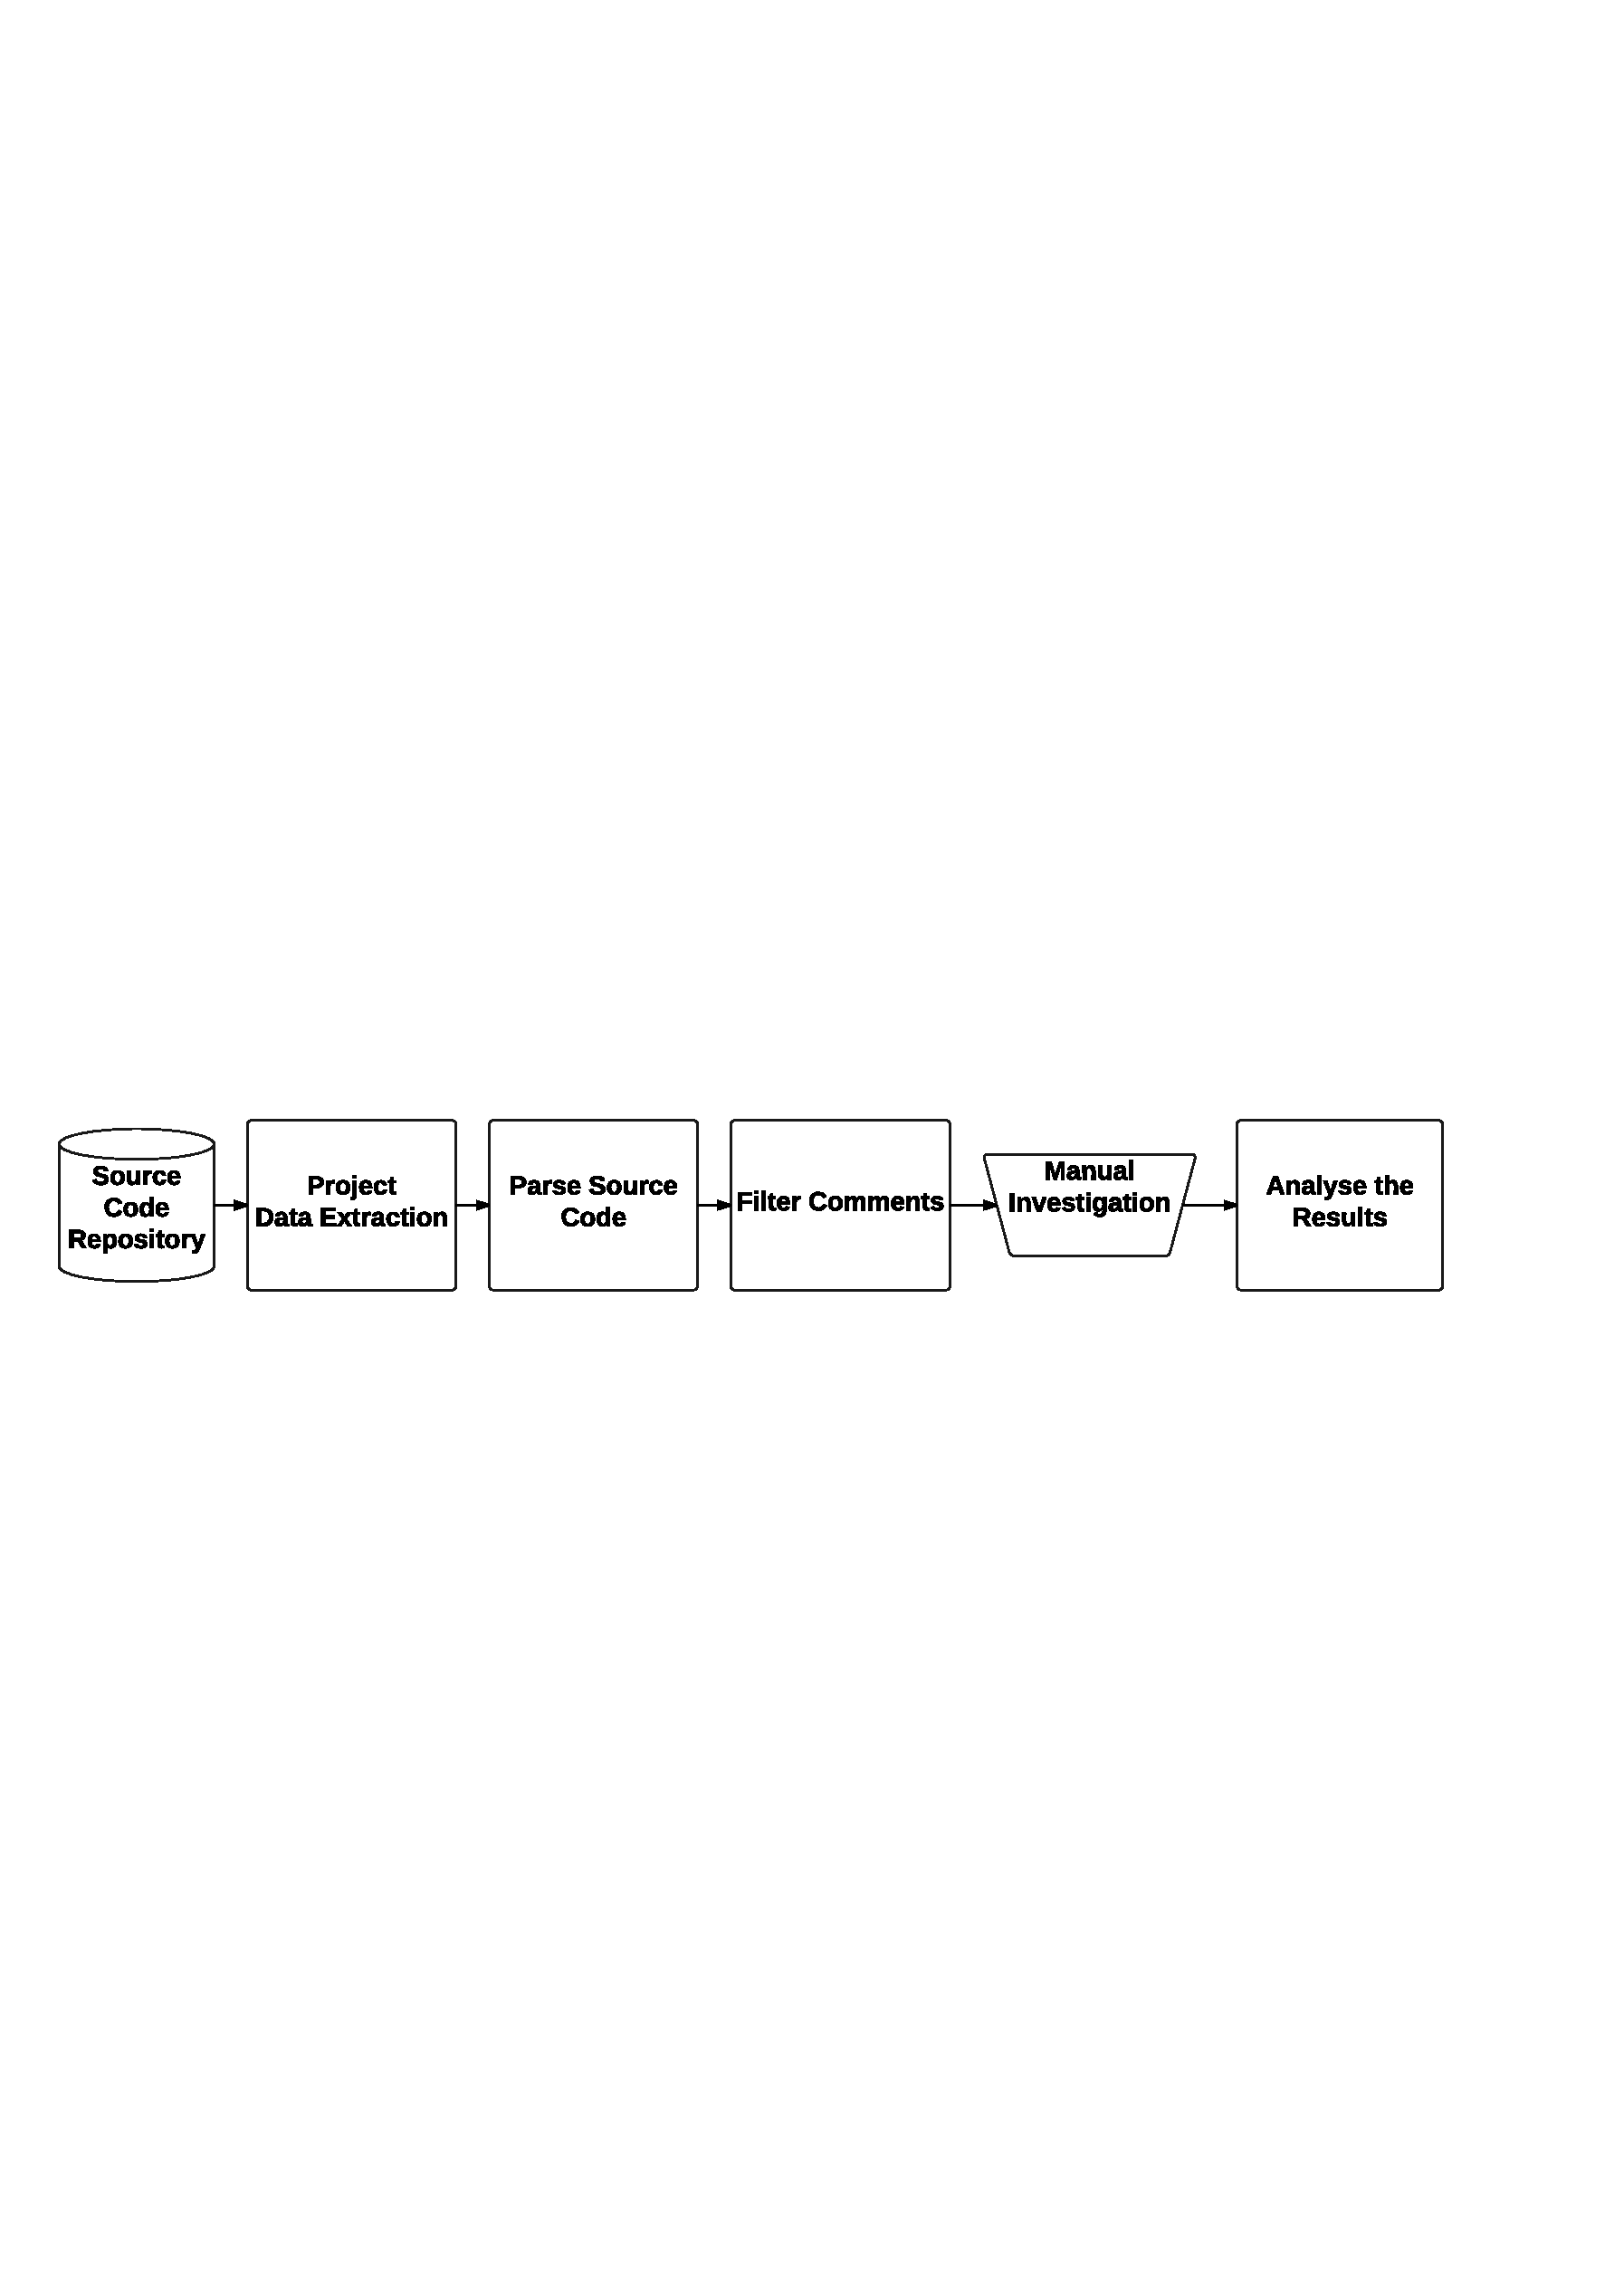
\includegraphics[width=1\textwidth]{figures/chapter3/approach.pdf}
  \caption{Approach overview}
  \label{chap3:fig:approach}
\end{figure*}

\begin{table*}[!hbt]
      \begin{center}
            \caption{Project Details}
            \label{chap3:tab:project_details}
            \begin{tabular}{l| c c r c c }
            \toprule
            \textbf{\thead{Project}}   & \textbf{\thead{Release}}  & \textbf{\thead{\# of \\classes}}   & \textbf{\thead{SLOC}}    & \textbf{\thead{\# of \\comments}}  & \textbf{\thead{\# of \\contributors}} \\ \midrule 
              Apache Ant       & 1.7.0             &  1,475                   & 115,881          & 21,587                   & 74  \\                       
              Apache Jmeter    & 2.10              &  1,181                   &  81,307          & 20,084                   & 33  \\                         
              ArgoUML          & 0.34              &  2,609                   & 176,839          & 67,716                   & 87  \\               
              Columba          & 1.4               &  1,711                   & 100,200          & 33,895                   & 9   \\                   
              JFreeChart       & 1.0.19            &  1,065                   & 132,296          & 23,474                   & 19  \\ \bottomrule
            \end{tabular}
      \end{center}
\end{table*}

The main goal of our study is to identify and quantify the different types of self-admitted technical debt found in source code comments. Figure \ref{chap3:fig:approach} shows an overview of our approach, and the following subsections detail each step of it.

\subsection{Project Data Extraction} 
\label{chap3:sub:project_data_extraction}

To perform our study, we obtain the source code of five open source projects, namely Apache Ant, Apache Jmeter, ArgoUML, Columba and JFreeChart. We chose the aforementioned projects, since they belong to different application domains, and vary in size (e.g., SLOC), and in the number of contributors.

Table \ref{chap3:tab:project_details} provides statistics about each one of the projects used in our study. We provide details about the release used, the number of classes, the total source lines of code (SLOC), the total extracted comments and the number of contributors. A source line of code contain at least one valid character, which is not blank spaces or source code comments. In our study, we only use the Java files to calculate the SLOC, and to do so, we use the tool SLOCCount \cite{wheeler2004:home}. 

The number of contributors was extracted from OpenHub, an on-line community and public directory that offers analytics, search services and tools for open source software \cite{Openhub:home}. It is important to notice that the number of comments shown for each project does not represent the number of commented lines, but rather the number of individual line, block, and Javadoc comments. In total, we obtained more than 166,756 comments, found in 8,041 Java classes.
 
\subsection{Parse Source Code} 
\label{chap3:sub:parse_source_code}

After obtaining the source code of all projects, we extract the comments from their source code. We use JDeodorant \cite{Tsantalis2008CSMR}, an open-source Eclipse plug-in, to parse the source code and extract the code comments. JDeodorant is capable of identify design flaws (i.e., bad smells) in Java projects, and suggest refactoring opportunities to solve them. JDeodrant uses the Eclipse AST framework to create an Abstract Syntax Tree (AST) map of the source code. The AST map contains detailed information about the project such as: the source code comments, its type (i.e., Block, Single-line or Javadoc), the line where each one of these comments begins and finishes. We extract the aforementioned information and store all comments in a relational database to facilitate the processing of the data.

\subsection{Filter Comments} 
\label{chap3:sub:filter_comments}

Source code comments can be used for different purposes in a project like giving context, as part of the documentation, to express thoughts, opinions and authorship, and in some cases, to remove source code from the program. Comments are used freely for developers and with few formalities, if any at all. This informal environment allows developers to bring to light opinions, insights and even confessions (e.g., self-admitted technical debt). 

As shown in prior work by Potdar and Shihab \cite{Potdar2014ICSME}, part of these comments can be identified as self-admitted technical debt, but they are not the majority of cases. With that in mind, we develop and apply 4 filtering heuristics to narrow down the comments eliminating the ones that are less likely to be classified as self-admitted technical debt.

To do so, we developed a Java based tool that reads from the database the data obtained by parsing the source code. Next, it executes the filtering heuristics and stores the result back in the database. The retrieved data contains information like the line number that a class/comment begins/ends and the type, considering the Java syntax, of the comment (i.e., Block, Single-line or Javadoc). With this information we process the filtering heuristics as described next.

We found that license comments are very not likely to contain self-admitted technical debt, and that license comments are commonly added before the declaration of the class. Therefore, we create a heuristic that removes comments that are placed before the class declaration. Since we know the line number that the class was declared we can easily check for comments that are placed before that line and remove them. In order to decrease the chances of removing a self-admitted technical debt comment while executing this filter we calibrated this heuristic to not remove comments containing one of task-reserved words (i.e., ``todo'', ``fixme'', or ``xxx'').

We also notice that some times developers make long comments, using multiple \emph{single-line} comments instead of a Block comment. This characteristic can hinder the understanding of the message. Consider the case that the reader (i.e., human or machine) analyze each one of these comments independently, the message would be incomplete and the meaning lost. To solve that problem, we create a heuristic that searches for consecutive single-line comments and groups them as one. We identify consecutive comments by subtracting the line number of both comments. If the result of the difference is equals a -1 we have a consecutive comment. For example, Single-line comment A is placed in line number 100 and Single-line comment B is placed in line 101. The subtraction of the line numbers will result in -1, therefore the comments are consecutive.
 
Similarly, is common to find commented source code across the projects, and this can be due to many different reasons. One of the possibilities is that the code is not being used, other is that the code is used for debug purposes only. Based on our analysis, commented source code does not have self-admitted technical debt. Our heuristic remove commented source code using a simple regular expression that captures typical Java code structures.

Lastly, when analyzing Javadoc comments we found that they rarely mention self-admitted technical debt. For the Javadoc comments that does mention self-admitted technical debt we notice that they usually contains one of the task-reserved words (i.e., ``todo'', ``fixme'', or ``xxx''). Based on this, our heuristic remove all comments of the type Javadoc unless they contain at least one of the task-reserved words. To do so, we create a simple regular expression that search for the task-reserved words before removing the comment.  

The steps mentioned above significantly reduced the number of comments in our dataset and helped us focus on the most applicable and insightful comments. For example, in the Apache Ant project, applying the above steps helped reduce the number of comments from 21,587 to 4,140 comments meaning that 19.17\% of the comments were kept for analysis. Table \ref{chap3:tab:filtering_heuristics_details} provides details for each one of the projects.

\begin{table}[!hbt]
      \begin{center}
            \caption{Filtering heuristics details}
            \label{chap3:tab:filtering_heuristics_details}
            \begin{tabular}{l| c c c}
            \toprule
            \textbf{\thead{Project}}   & \textbf{\thead{Total \# of\\ comments}}  & \textbf{\thead{\# of \\comments \\after filtering}} & \textbf{\thead{\%  of \\TD-related \\comments}}\\ \midrule 
              Apache Ant       & 21,587                & 4,140                   & 19.17 \% \\ 
              Apache Jmeter    & 20,084                & 8,163                   & 40.64 \% \\
              ArgoUML          & 67,716                & 9,788                   & 14.45 \% \\              
              Columba          & 33,895                & 6,569                   & 19.38 \% \\
              JFreeChart       & 23,474                & 4,436                   & 18.89 \% \\ \bottomrule
            \end{tabular}
      \end{center}
\end{table}

\subsection{Manual Classification} 
\label{chap3:sub:manual_classification}

To classify the comments, we developed a Java based tool that shows one comment at a time and gives a list of possible classifications that can be manually assigned to the comment. The list of possible classifications is based on previous work by Alves \textit{et al.}~\cite{Alves2014MTD}. After applying the different filtering steps, we successfully classified 33,093 comments. The more than 33 thousand comments were classified into five different types of self-admitted technical debt, i.e., design debt, defect debt, documentation debt, requirement debt and test debt.

The first author who made the classification has more than 8 years of experience working in the industry as a software engineer, during this time he designed, implemented and maintained several programs using, in particular the Java programming language. He developed solid skills in object orientated programming and design patterns. We consider that these qualifications provide the necessary background to conduct the manual classification of the comments.   

\section{Case Study Results}
\label{chap3:sec:results}

The goal of our study is to classify and quantify the different types of self-admitted technical debt. To do so, we divide our study in two parts first, we manually read trough all comments identifying self-admitted technical debt among them. Once identified, the self-admitted technical debt, is classified into different types. Second, we quantify these comments identifying the most common types. Our case study is formalized with the following research question:

\vspace{3mm}
\noindent\chapterIIIrqi
\vspace{3mm}

\noindent\textbf{Motivation:} As shown in previous work \cite{Potdar2014ICSME}, self-admitted technical can be an indicator of non-optimal solutions. However, technical debt is a general term, and there are many different types of technical debt \cite{Alves2014MTD}. Although we know that self-admitted technical exists, the different types of self-admitted technical debt are still unknown. For example, are we able to detect documentation debt from code comments? Answering this question is important as different types of debt have different approaches to be solved, and therefore each different type may need a tailored solution. It also helps us understand the opportunities and limitations of using code comments to detect technical debt. 

\vspace{1mm}
\noindent\textbf{Approach:} To identify the different types of debt found in the comments we manually read through source code comments as described in Section \ref{chap3:sec:approach}. While examining the comments we classify each comment by the nature of the debt, using the descriptions provided by Alves \textit{et al.} as a guideline. 

During the classification we notice that some comments can be classified in more than one type of debt (e.g., a comment reporting a design debt can also be causing an unexpected behavior, which is defect debt). Although this is an ambiguous situation, and may have different interpretations depending of who is reading the comments, we defined that each comment would have just one classification type for the sake of clarity. 

To mitigate the chance of misclassifying these comments, we take in consideration the more meaningful type for each comment in a given scenario. To do so, whenever a case like this occurred, we did a more detailed investigation (i.e., by examining the source code and any available documentation). In total we read and classified 33,093 comments from five open source projects. The classification took approximately 95 hours and was performed by the first author of the paper. 

\vspace{1mm}
\noindent\textbf{Results:} We found five different types of self-admitted technical debt. Below, we list the different types of technical debt that we were able to detect and provide example comments to help the reader grasp the different types of self-admitted technical debt comments.


\begin{itemize}
  \item \textbf{Self-admitted design debt:} These comments indicate that there is a problem with the design of the code. They can be comments about misplaced code, lack of abstraction, long methods, poor implementation, workarounds or a temporary solution. Lets consider the following comments:
  
  \vspace{1mm}
  \begin{displayquote}
     \textit{``TODO: - This method is too complex, lets break it up''} - [from ArgoUml]
     
     \vspace{1mm}

     \textit{``/* TODO: really should be a separate class */''} - [from ArgoUml]
  \end{displayquote}
  \vspace{1mm}

These comments are clear examples of what we consider as self-admitted \emph{design debt}. In the above comments, the developers state what needs to be done in order to improve the current design of the code. Although the above comments are easy to understand, during our study we came across more challenging comments that expressed design problems in an indirect way. For example: 
  
  \vspace{1mm}
  \begin{displayquote}
     \textit{``// I hate this so much even before I start writing it. // Re-initialising a global in a place where no-one will see it just // feels wrong.  Oh well, here goes.''} - [from ArgoUml]

     \vspace{1mm}

     \textit{``//quick \& dirty, to make nested mapped p-sets work:''} - [from Apache Ant]
  \end{displayquote}
  \vspace{1mm}

In the above example comments the authors are certain to be implementing code that does not represent the best solution. Intuitively, we know that kind of implementation will degrade the design of the code and should be avoided. 

  \vspace{1mm}
  \begin{displayquote}
      \textit{``// probably not the best choice, but it solves the problem of // relative paths in CLASSPATH''} - [from Apache Ant]

      \vspace{1mm}

      \textit{``//I can't get my head around this; is encoding treatment needed here?''} - [from Apache Ant]
  \end{displayquote}
  \vspace{1mm}

The above comments expressed doubt and uncertainty when implementing the code and were considered as self-admitted design debt as well.

\item \textbf{Self-admitted defect debt:} In defect debt comments the author states that a part of the code does not have the expected behavior, meaning that there is a defect in the code. 
  
  \vspace{1mm}
  \begin{displayquote}
      \textit{``// Bug in above method''} - [from Apache Jmeter]

      \vspace{1mm}

      \textit{``// WARNING: the OutputStream version of this doesn't work!''} - [from ArgoUml]
  \end{displayquote}
  \vspace{1mm}
  
As shown in these examples there are defects that are known by the developers, but for some reason is not fixed yet. 

  \item \textbf{Self-admitted documentation debt:} In the documentation debt comments the author express that there is no proper documentation supporting that part of the program.
  
  \vspace{1mm}
  \begin{displayquote}
    \textit{``**FIXME** This function needs documentation''} - [from Columba]
    
    \vspace{1mm}
    
    \textit{``// TODO Document the reason for this''} - [from Apache Jmeter]
  \end{displayquote}
  \vspace{1mm}
  
  Here, the developers clearly recognize the need to document their code, however, for some reason they do not document it yet.
  
  \item \textbf{Self-admitted requirement debt:} Requirement debt comments express incompleteness of the method, class or program as observed in the following comments:
  
  \begin{displayquote}
    \textit{``/TODO no methods yet for getClassname''} - [from Apache Ant]
    
    \vspace{1mm}
    
    \textit{``//TODO no method for newInstance using a reverse-classloader''} - [from Apache Ant]

    \vspace{1mm}
    
    \textit{``TODO: The copy function is not yet * completely implemented - so we will  * have some exceptions here and there.*/''} - [from ArgoUml]  
    
  \end{displayquote}
  \vspace{1mm}  
  
The last example shows a comment that could be considered as having more than one type of debt. (i.e., requirement debt and defect debt), but as mentioned in the classification approach, we choose to maintain one type only for each comment. Based on our understanding, the defect debt expressed in the comment would not exist if the requirement debt did not exists. Therefore, the main debt in this comment is a requirement debt (i.e., incomplete implementation of the copy function). 
      
  \vspace{1mm}
  \item \textbf{Self-admitted test debt:} Test debt comments are the ones that express the need for implementation or improvement of the current tests. As shown in the examples below, test debt comments are very straight forward in their meaning. 
  
  \begin{displayquote}
    \textit{``// TODO - need a lot more tests''} - [from Apache Jmeter]
    
    \vspace{1mm}
    
    \textit{``//TODO enable some proper tests!!''} - [from Apache Jmeter]
  \end{displayquote}
  \vspace{1mm}  
    
\end{itemize}

After classifying the comments, we notice that not all of the types mentioned in by Alves \emph{et al.}~\cite{Alves2014MTD} could be found. We argue that some types like people debt or infrastructure debt are less probable to appear in source code comments. Other types such as build debt could not be found because we are examining comments in Java classes only, not taking in consideration build scripts that are usually written in other languages (e.g., Maven and Ant use XML files as build scripts). 

\conclusionbox{We find five different types of self-admitted technical debt, i.e., design debt, defect debt, documentation debt, requirement debt and test debt.}

\begin{figure*}[thb!]
  \centering
  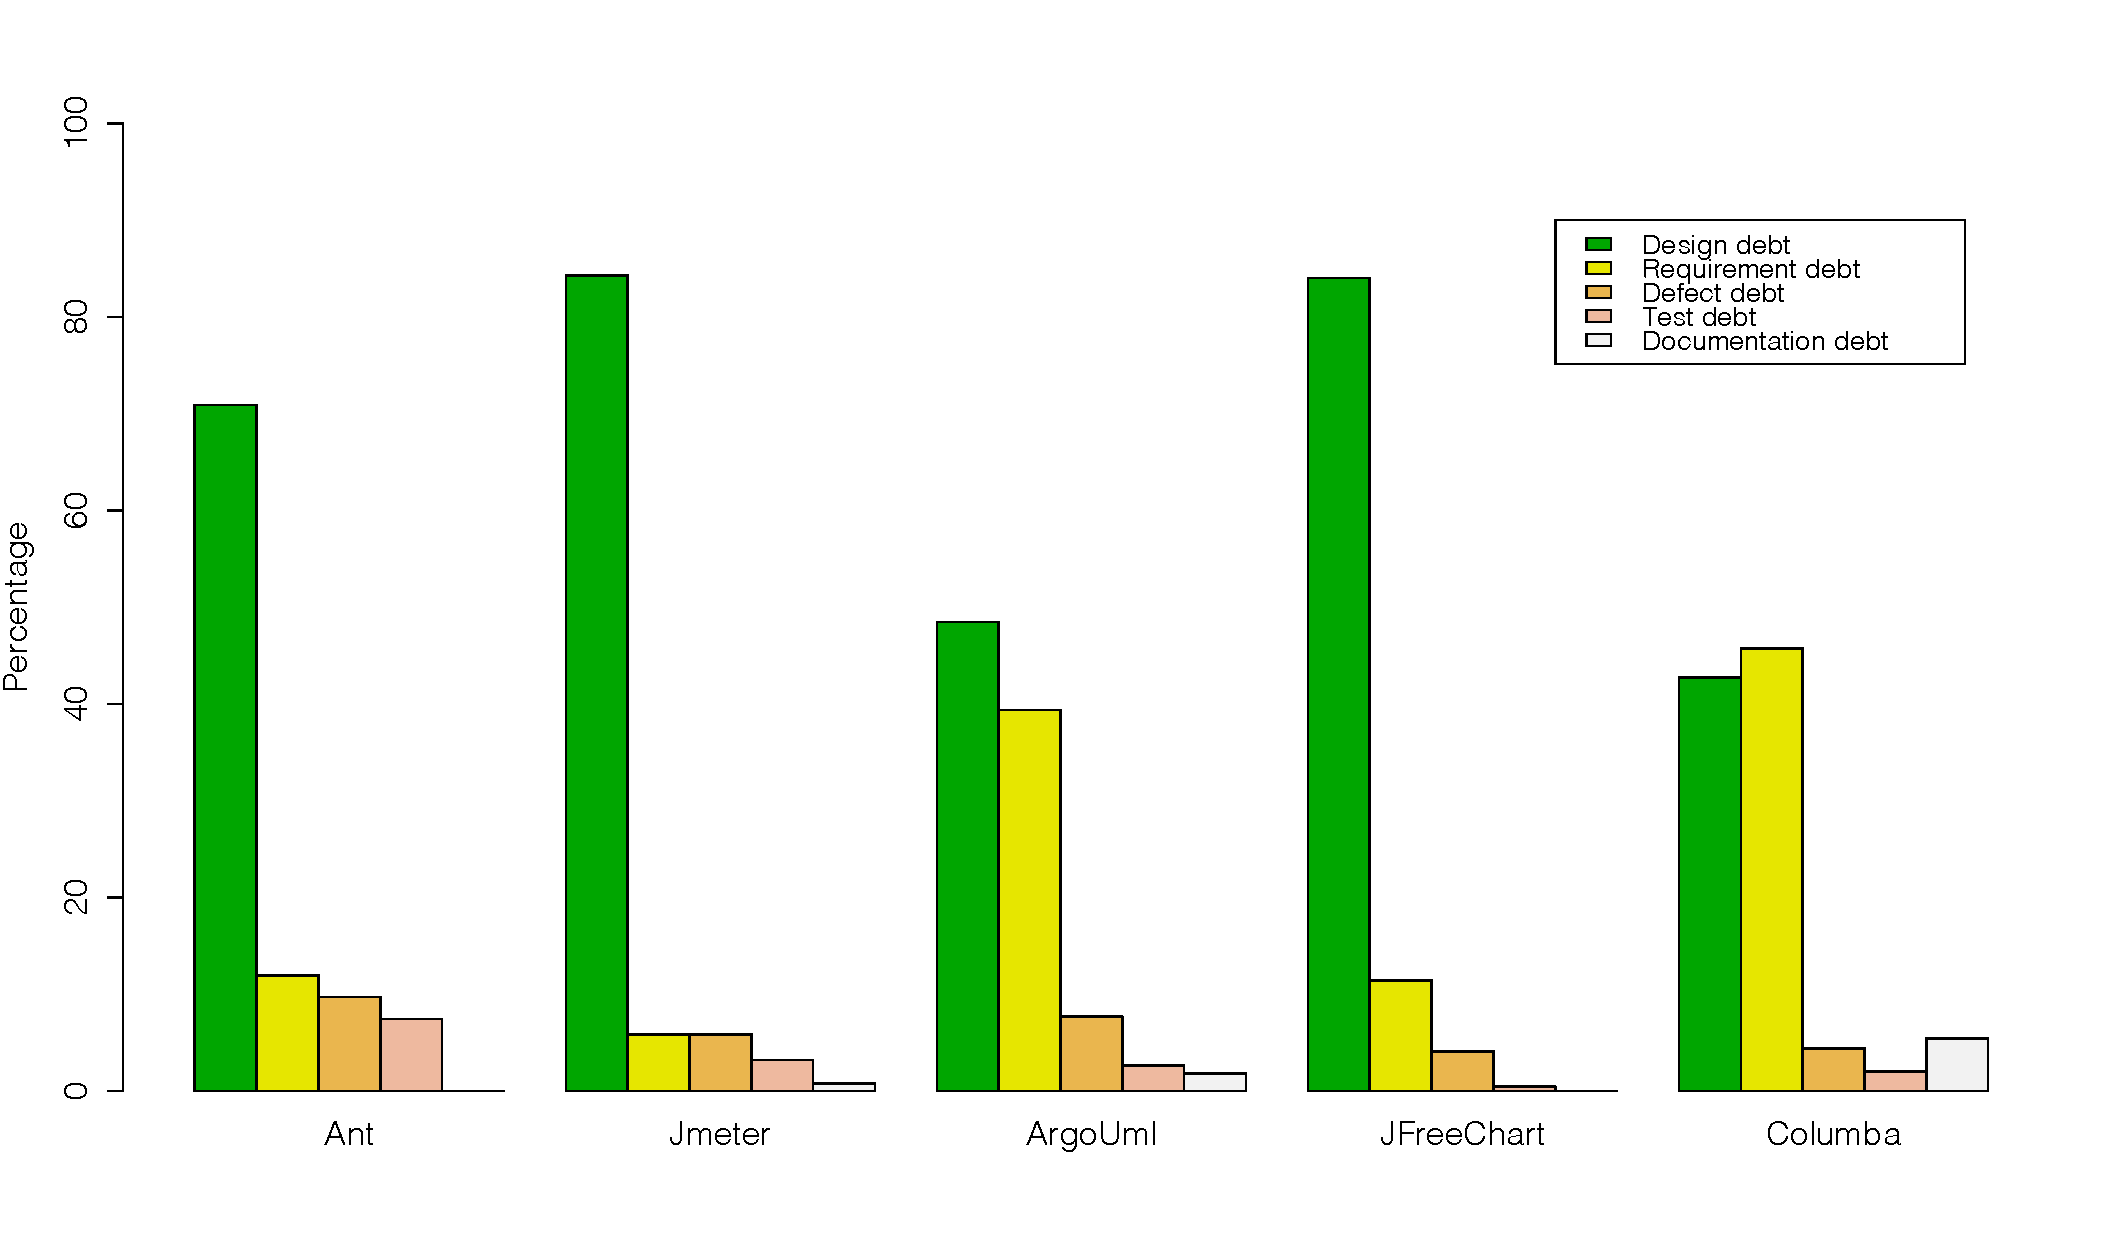
\includegraphics[width=1\textwidth]{figures/chapter3/technical_debt_distribution.pdf}
  \caption{Self-admitted technical debt types distribution}
  \label{chap3:fig:satd_distribution}
\end{figure*}

In addition to determining the different type of self-admitted technical debt, we would like to quantify the different types. Doing so will help us understand the strengths and weaknesses of using code comments to detect technical debt. After analyzing the more than 33K comments, we found that only 2,457 comments are self-admitted technical debt comments, representing 7.42\% (i.e., $\frac{2457}{33093}$) of all the classified comments. The percentage of self-admitted technical debt found for each project is presented in Table~\ref{tab:total_self_admitted_per_project}. ArgoUml is the project with the highest percentage of self-admitted technical debt and Apache Ant has the lowest percentage, amounting to 16.8\% and 3.2\% respectively.

\begin{table}[!hbt]
     \begin{center}
           \caption{Self-admitted technical debt per project}
           \label{tab:total_self_admitted_per_project}
           \begin{tabular}{l| c c c }
           \toprule
           \textbf{\thead{Project}}      & \textbf{\thead{\# of analyzed \\comments}}     & \textbf{\thead{\# of \\self-admitted TD \\comments}} & \textbf{\thead{\% of \\self-admitted TD\\ per project}} \\ \midrule 
             Apache Ant          & 4,140                          & 134                                & 3.2  \\                                   
             Apache Jmeter       & 8,163                          & 375                                & 4.6  \\                                   
             ArgoUML             & 9,788                          & 1,653                              & 16.8 \\                                   
             Columba             & 6,569                          & 295                                & 4.4 \\                                   
             JFreeChart          & 4,433                          & 219                                & 4.9  \\ \bottomrule
           \end{tabular}
     \end{center}
\end{table}

Figure \ref{chap3:fig:satd_distribution} shows the percentage of each type of self-admitted technical debt across the projects. Since each project has a different number of comments we normalized the data, presenting the percentages of the different types rather than the raw numbers. For example, if a project has 100 self-admitted technical debt comments and 10 where design debt type, we say that the project has 10\% of self-admitted design technical debt. 

Analyzing the Figure \ref{chap3:fig:satd_distribution} we find that self-admitted design debt is the most common in 4 out of 5 projects. Self-admitted design technical debt values ranged from 42\%, in Columba project with the lowest percentage, to 84\% in Jmeter and JFreeChart, projects with the highest percentage. The second most frequent type is self-admitted requirement debt with values between 5\% and 45\%, followed by self-admitted defect technical debt making up between 4\% to 9\% of the comments. Self-admitted test technical debt ranged from 0\% to 7\% whereas self-admitted documentation debt had only 0\% to 5\% of the comments.     

We notice that Columba and ArgoUml have the highest occurrences of self-admitted requirement debt. Columba is a email client application written in Java, which has 9 contributors \cite{Openhub:home}, and a considerable number of classes 1,711. It is reasonable to think that developers have limited time to develop features. Therefore, leaving comments of features that need to be implemented in the future (i.e., requirement debt) is more likely. 

ArgoUml has a high number of contributors i.e., 87 and yet has a hight number of self-admitted requirement debt. Analyzing the comments we notice that there occurrences about the need of support for internationalization and other comments express the need to implement code to make features compatible with newer versions of the UML language. 

Based on that we argue that coupling with external changes that are inherent of the application domain and the adoption of the tool from users all over the world \cite{Openhub:home} had increased the number of self-admitted requirement debt. 

\conclusionbox{We find that the majority of the self-admitted technical debt comments are design debt, which ranged from 42\% to 84\% across the projects. The second most frequent type was requirement debt that ranged from 5\% to 45\%. The remaining types have low frequency if considered that they represented less than 10\% of the occurrences}

\section{Threats to Validity}
\label{chap3:sec:threats_to_validity}

\noindent\textbf{Internal validity} consider the relationship between theory and observation, in case the measured variables do not measure the actual factors. To classify the source code comments we heavily depended on manual process due the fact that comments are written in natural language and therefore difficult to analyze by a machine. Like any human activity, our manual classification is subject to personal bias and subjectivity. To reduce this bias, in the future, we will ask to other researchers of our lab to classify the dataset as well, verifying and discussing possible divergences of opinion. This is important as changes in this dataset may impact our findings. 

When performing our study, we used well-commented Java projects. Since our technique heavily depends on code comments, our results may be impacted by the quantity and quality of comments in a software project. To alleviate the threat, we examined multiple projects. Moreover, there is a risk of removing self-admitted technical debt comments while filtering license comments. To mitigate this risk we do not remove comments that contain one of task-reserved words (i.e., ``todo'', ``fixme'', or ``xxx'').

\noindent \textbf{External validity} consider the generalization of our findings. All of our findings were derived from comments in open source projects. To minimize external validity, we chose open source projects from different domains. That said, our results may not generalize to other open source or commercial projects. In particular, our results may not generalize to projects that have a low number or no comments. Other than that, we only analyze projects written in Java, therefore the results obtained may not generalize to projects written in other languages.

\section{Conclusion and Future Work}
\label{chap3:sec:conclusion}

The term technical debt is being used for practitioners and researchers in the software engineer community to express shortcuts and workarounds employed in software projects. These shortcuts will most often impact the maintainability of the project hindering the development if not addressed properly. Our work explore specifically self-admitted technical debt, that is the technical debt deliberately introduced by the developers and reported through source code comments.

In our study we analyzed the comments of 5 open source projects which are Apache Ant, Apache Jmeter, ArgoUml , Columba and JFreeChart. These projects are considered well commented and they belong to different application domains. We used them to understand the characteristics of self-admitted technical debt types creating a rich dataset with more than 33,093 classified comments.

We find that self-admitted technical debt can be classified into five types: design debt, defect debt, documentation debt, requirement debt and test debt. We also provide concrete examples of each one of the mentioned types and the rationale to classify them as it was. Moreover, we find that the majority of the self-admitted technical debt comments are design debt. Design debt ranged from 42\% to 84\% across the projects. The second most frequent type was requirement debt ranging from 5\% to 45\%. Based on this result, we can say that the self-admitted technical debt types that developers admit to the most are related with the design of the project, potentially indicating that developers feel the need to admit and be forthcoming about such debt. Examining the reasons for these types of debt is an interesting future direction that we plan to pursue.

Moreover, in this chapter we explained our filtering heuristics to remove comments that are not likely to have technical debt. In the next chapter we leveraged all the knowledge obtained by this first study. We will explain in details how we expanded the size of our dataset, doubling the amount of projects being analyzed, and consequently, broadening the application domains involved in the study.

This dataset is then used to train a NLP classifier that is able to automatically identify \SATD. To understand how good our approach is in identifying \SATD we compare the performance that we obtained with the performance of two other baselines, one of these baselines is the current state-of-the-art. 


\chapter{Proposing an Approach to Automatically Identify Self-Admitted Technical Debt}
\label{chapter4}
% -*- root: cuthesis_masters.tex -*-
\section{Introduction}
\label{chap4:sec:introduction}

Developers often have to deal with conflicting goals that require software to be delivered quickly, with high quality, and on budget. In practice, achieving all of these goals at the same time can be challenging, causing a tradeoff to be made. Often, these tradeoffs lead developers to take \emph{shortcuts} or use \emph{workarounds}. Although such shortcuts help developers in meeting their short-term goals, they may have a negative impact in the long-term.

Technical debt is a metaphor coined to express sub-optimal solutions that are taken in a software project in order to achieve some short-term goals~\cite{Cunningham1992WPM}. Generally, these decisions allow the project to move faster in the short-term, but introduce an increased cost (i.e., debt) to maintain this software in the long run~\cite{Seaman2011,Kruchten2013IWMTD}.  Prior work has shown that technical debt is widespread in the software domain, is unavoidable, and can have a negative impact on the quality of the software~\cite{Lim2012Software}. 

Technical debt can be deliberately or inadvertently incurred~\cite{MartinFowler:TechnicalDebtQuadrant}. Inadvertent technical debt is technical debt that is taken on unknowingly. One example of inadvertent technical debt is architectural decay or architectural drift. To date, the majority of the technical debt work has focused on inadvertent technical debt~\cite{Nord2012WICSA}. On the other hand, deliberate technical debt, is debt that is incurred by the developer with knowledge that it is being taken on. One example of such deliberate technical debt, is self-admitted technical debt, which is the focus of our paper.

Due to the importance of technical debt, a number of studies empirically examined technical debt and proposed techniques to enable its detection and management. Some of the approaches analyze the source code to detect technical debt, whereas other approaches leverage various techniques and artifacts, e.g., documentation and architecture reviews, to detect documentation debt, test debt or architecture debt (i.e., unexpected deviance from the initial architecture)~\cite{Alves2016IST,Xiao2016ICSE}.

The main findings of prior work are three-fold. First, there are different types of technical debt, e.g., defect debt, design debt, testing debt, and that among them design debt has the highest impact~\cite{Alves2014MTD,Marinescu2012IBM}. Second, static source code analysis helps in detecting technical debt, (i.e., code smells)~\cite{Marinescu2004ICSM,Marinescu2010CSMR,Zazworka2013CSE}. Third, more recently, our work has shown that it is possible to identify technical debt through source comments, referred to as  \SATD~\cite{Potdar2014ICSME}, and that design and requirement debt are the most common types of \SATD~\cite{Maldonado2015MTD}.

The recovery of technical debt through source code comments has two main advantages over traditional approaches based on source code analysis. First, it is more lightweight compared to source code analysis, since it does not require the construction of Abstract Syntax Trees or other more advanced source code representations. For instance, some code smell detectors that also provide refactoring recommendations to resolve the detected code smells~\cite{Tsantalis2011TSE,Tsantalis2015TSE} generate computationally expensive program representation structures, such as program dependence graphs~\cite{Graf2010SCAM}, and method call graphs~\cite{Ali2012ECOOP} in order to match structural code smell patterns and compute metrics. On the other hand, the source code comments can be easily and efficiently extracted from source code files using regular expressions. Second, it does not depend on arbitrary metric threshold values, which are required in all metric-based code smell detection approaches. Deriving appropriate threshold values is a challenging open problem that has attracted the attention and effort of several researchers~\cite{Oliveira2014CSMR,Fontana2015WETSoM,Fontana2015EMSE}. As a matter of fact, the approaches based on source code analysis suffer from high false positive rates~\cite{Fontana2016SANER} (i.e., they flag a large number of source code elements as problematic, while they are not perceived as such by the developers), because they rely only on the structure of the source code to detect code smells without taking into account the developers' feedback, the project domain, and the context in which the code smells are detected.

However, relying solely on the developers' comments to recover technical debt is not adequate, because developers might be unaware of the presence of some code smells in their project, or might not be very familiar with good design and coding practices (i.e., inadvertent debt).
As a result, the detection of technical debt through source code comments can be only used as a complementary approach to existing code smell detectors based on source code analysis.
We believe that \SATD can be useful to prioritize the \textit{pay back} of debt (i.e., develop a \textit{pay back} plan), since the technical debt expressed in the comments written by the developers themselves is definitely more relevant to them.

Despite the advantages of recovering technical debt from source code comments, the research in \SATD, thus far, heavily relies on the manual inspection of code comments. The current-state-of-the art approach~\cite{Potdar2014ICSME} uses 62 comment patterns (i.e., words and phrases) derived after the manual examination of more than 100K comments. The manual inspection of code comments is subject to reader bias, time consuming and, as any other manual task, susceptible to errors. These limitations in the identification of \SATD comments makes the current state-of-the-art approach difficult to be applied in practice.

Therefore, in this paper we investigate the efficiency of using Natural Language Processing (NLP) techniques to automatically detect the two most common types of \SATD, i.e., design and requirement debt. We analyze ten open source projects from different application domains, namely, Ant, ArgoUML, Columba, EMF, Hibernate, JEdit, JFreeChart, JMeter, JRuby and SQuirrel SQL. We extract and classify the source comments of these projects. Then, using the classified dataset we train a maximum entropy classifier using the Stanford Classifier tool~\cite{manning2003optimization} to identify design and requirement \SATD.
The advantages of the maximum entropy classifier over keyword-based and pattern-based approaches, such as comment patterns, are twofold. First, the maximum entropy classifier automatically extracts the most important features (i.e., words) for each class (i.e., design \SATD, requirement \SATD, and without technical debt) based on a classified training dataset given as input. Second, the maximum entropy classifier, apart from finding features that contribute positively to the classification of a comment in a given class, also finds features that contribute negatively to the classification of a comment in a given class.

We perform a leave-one-out cross-project validation (i.e., we train on nine projects and test on one project). Our results show that we are able to  achieve an average F1-measure of 0.620 when identifying design \SATD, and an average F1-measure of 0.403 when identifying requirement \SATD. We compare the performance of our approach to the state-of-the-art approach used to detect \SATD~\cite{Potdar2014ICSME}. Our results show that on average, we outperform the state-of-the-art by 2.3 times, when detecting design debt, and by 6 times when detecting requirement debt.

To better understand how developers express technical debt we analyze the 10 most prevalent words appearing within \SATD comments. 
We find that the top design debt words are related to sloppy or mediocre source code. For example, words such as `hack', `workaround' and `yuck!' are used to express design \SATD. On the other hand, for requirement debt, words indicating the need to complete a partially implemented requirement are the best indicators. For example, words such as `todo', `needed' and `implementation' are strong indicators of requirement debt. 

Finally, to determine the most efficient way to apply our approach, we analyze the amount of training data necessary to effectively identify \SATD. We find that training datasets using 23\% of the available data can achieve a performance equivalent to 90\% of the maximum F1-measure score for both design and requirement \SATD. Similarly, 80\% of the maximum F1-measure can be achieved using only 9\% of the available data for design \SATD, and 5\% for requirement \SATD.

The main contributions of our work are the following:

\begin{itemize}
  \item We provide an automatic, NLP-based, approach to identify design and requirement \SATD.
  \item We examine and report the words that best indicate design and requirement \SATD.
  \item We show that using a small training set of comments, we are able to effectively detect design and requirement \SATD.
  \item We make our dataset publicly available\footnote{https://github.com/maldonado/tse\_satd\_data}, so that others can advance work in the area of \SATD.
\end{itemize}

The rest of the chapter is organized as follows. Section \ref{chap4:sec:approach} describes our approach. We setup our experiment and present our results in Section \ref{chap4:experiment_results}. We discuss the implications of our findings in Section \ref{chap4:sec:discussion}. In Section \ref{chap4:sec:related_work} we present the related work. Section \ref{chap4:sec:threats_to_validity} presents the threats to validity and Section \ref{chap4:sec:conclusion} presents our conclusions and future work.  

\section{Approach}
\label{chap4:sec:approach}

\begin{figure*}[thb!]
  \centering
  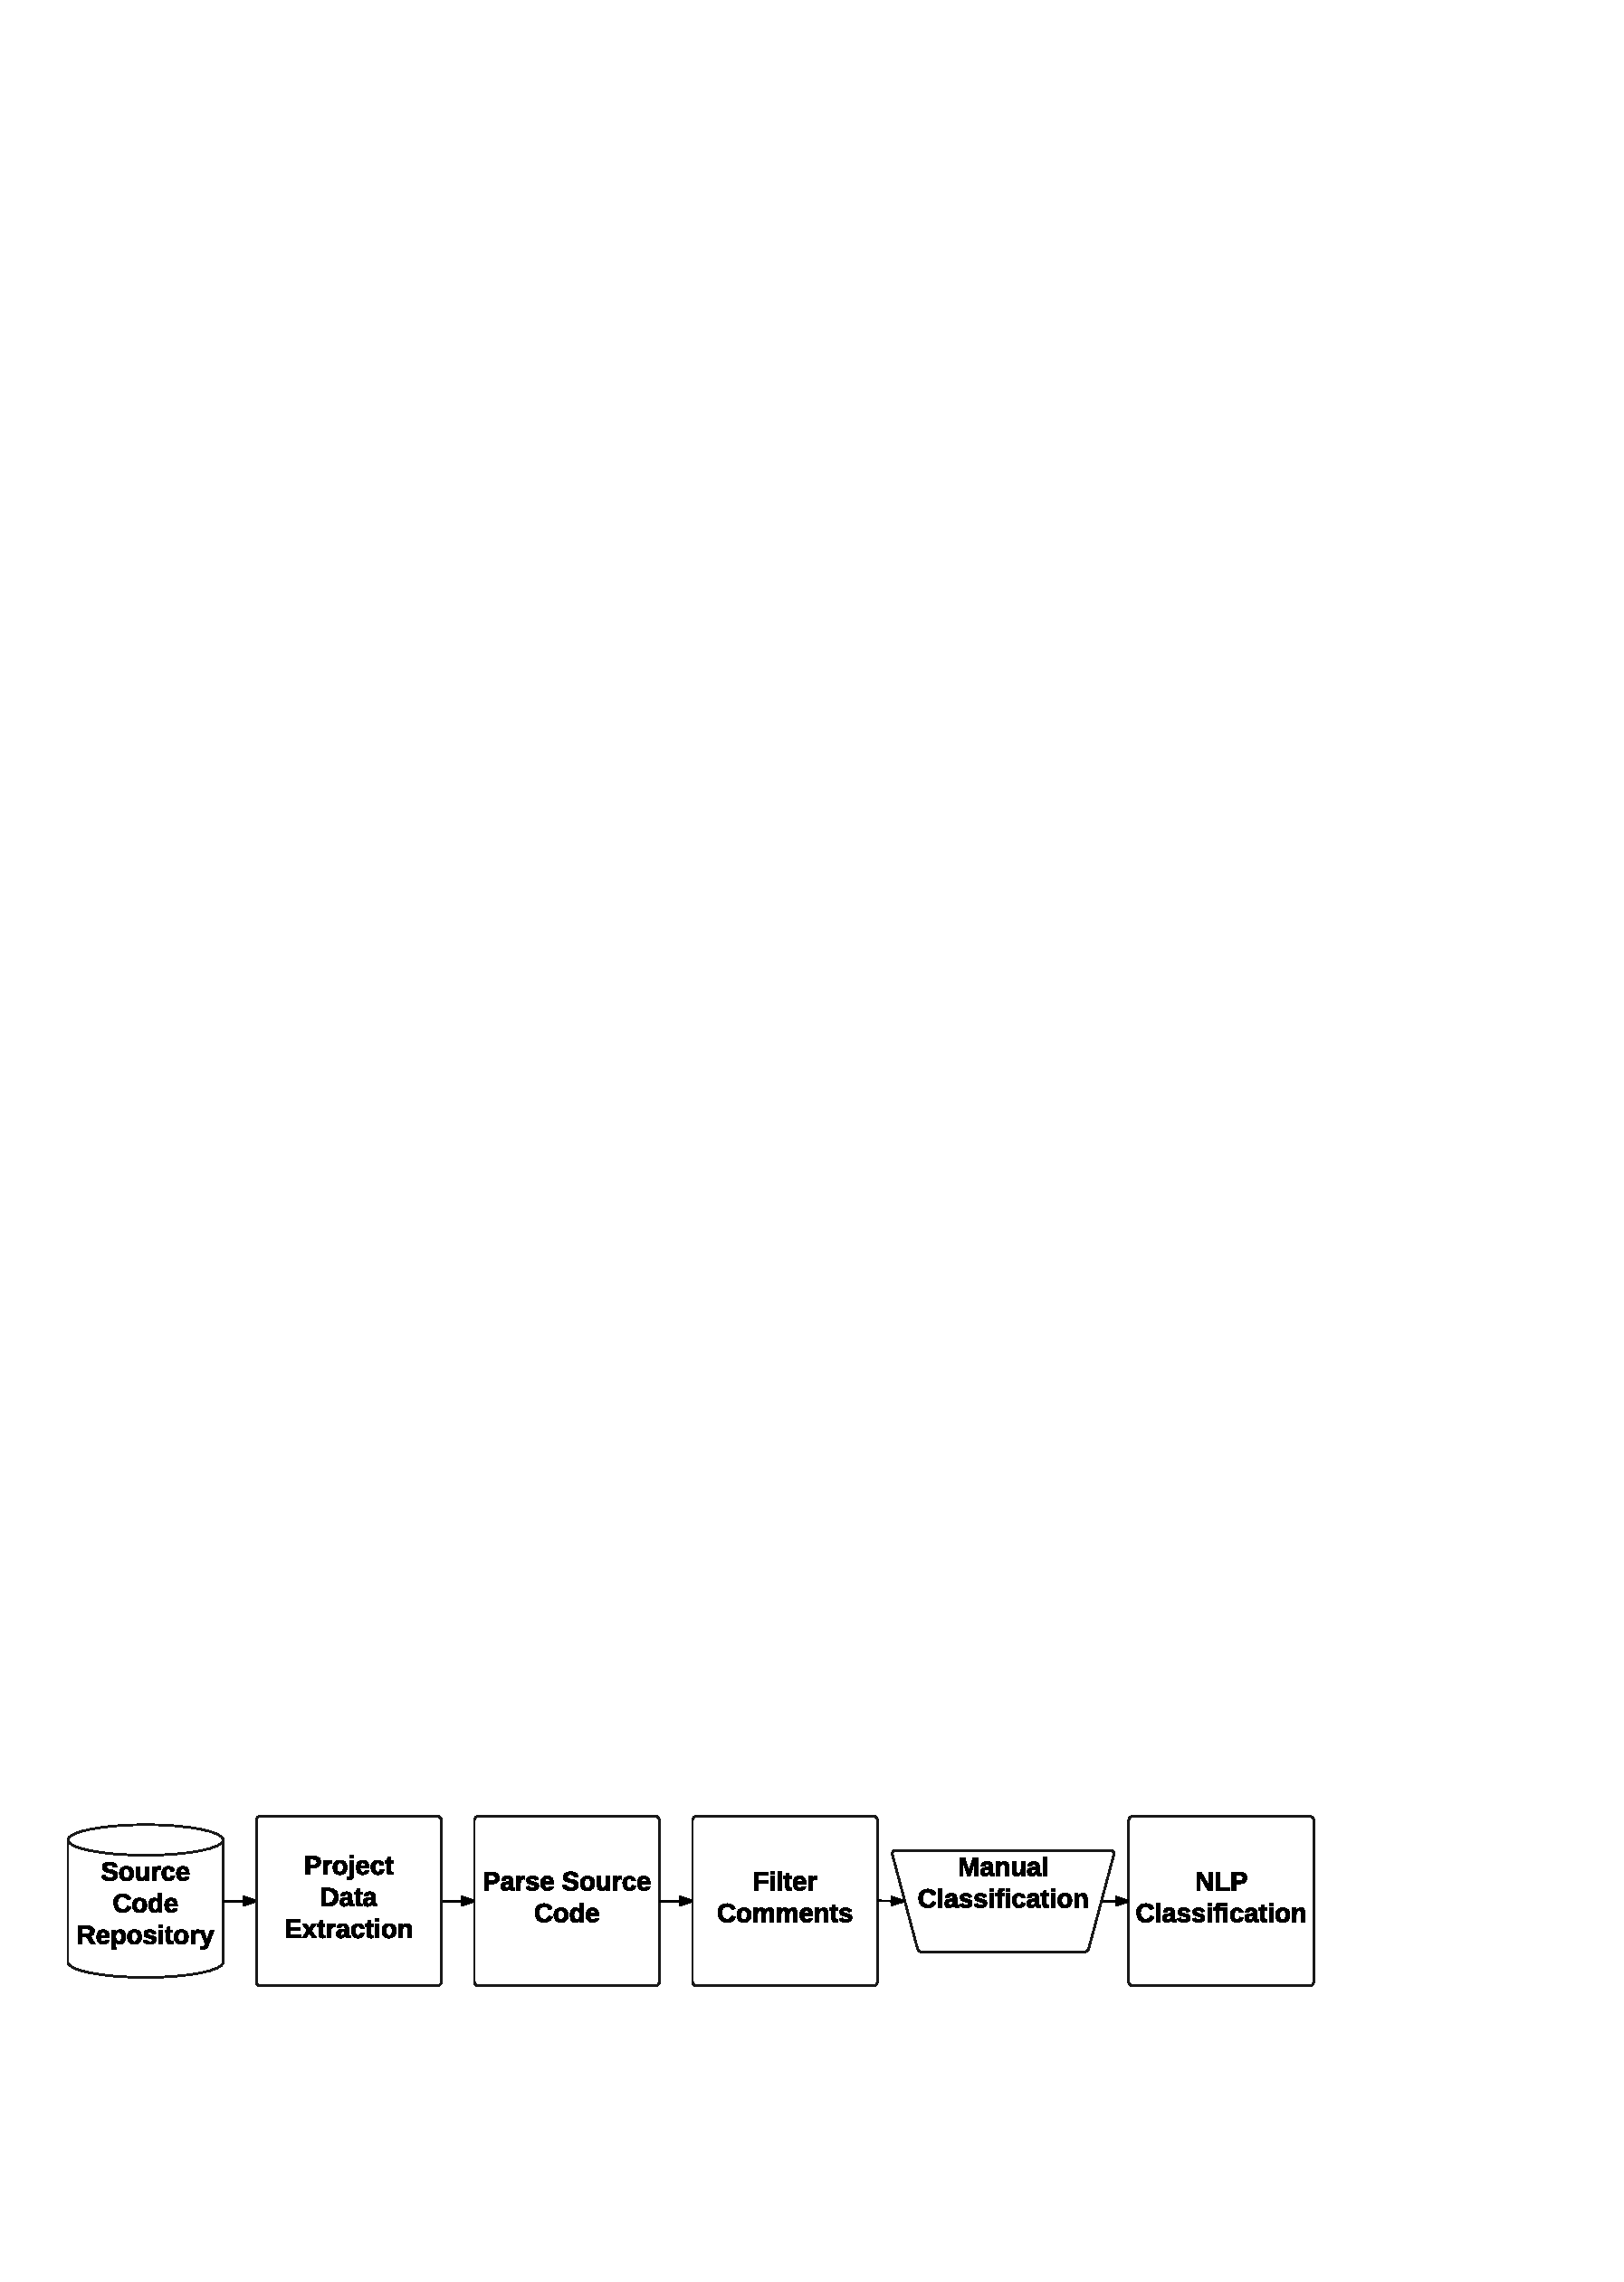
\includegraphics[width=1\textwidth]{figures/chapter4/approach_reviwed.pdf}
  \caption{NLP Based Approach Overview}
  \label{chap4:fig:approach}
\end{figure*}

The main goal of our study is to automatically identify \SATD through source code comments. To do that, we first extract the comments from ten open source projects. Second, we apply five filtering heuristics to remove comments that are irrelevant for the identification of \SATD  (e.g., license comments, commented source code and Javadoc comments). After that, we manually classify the remaining comments into the different types of \SATD (i.e., design debt, requirement debt, defect debt, documentation debt and test debt). Lastly, we use these comments as training data for the maximum entropy classified and use the trained model to detect \SATD from source code comments. Figure~\ref{chap4:fig:approach} shows an overview of our approach, and the following subsections detail each step.

\subsection{Project Data Extraction}
\label{chap4:sub:data_extraction}

To perform our study, we need to analyze the source code comments of software projects. Therefore, we focused our study on ten open source projects: Ant is a build tool written in Java, ArgoUML is an UML modeling tool that includes support for all standard UML 1.4 diagrams, Columba is an email client that has a graphical interface with wizards and internationalization support, EMF is a modeling framework and code generation facility for building tools and other applications, Hibernate is a component providing Object Relational Mapping (ORM) support to applications and other components, JEdit is a text editor written in Java, JFreeChart is a chart library for the Java platform, JMeter is a Java application designed to load functional test behavior and measure performance, JRuby is a pure-Java implementation of the Ruby programming language and SQuirrel SQL is a graphical SQL client written in Java. We selected these projects since they belong to different application domains, are well commented, vary in size, and in the number of contributors. 
    
Table~\ref{chap4:tab:project_details} provides details about each of the projects used in our study. The columns of Table~\ref{chap4:tab:project_details} present the release used, followed by the number of classes, the total source lines of code (SLOC), the number of contributors, the number of extracted comments, the number of comments analyzed after applying our filtering heuristics, and the number of comments that were classified as \SATD together with the percentage of the total project comments that it represent.
The final three columns show the percentage of \SATD comments classified as design debt, requirement debt, and all other remaining types of debt (i.e., defect, documentation and test debt), respectively. 

Since there are many different definitions for the SLOC metric we clarify that, in our study, a source line of code contains at least one valid character, which is not a blank space or a source code comment. In addition, we only use the Java files to calculate the SLOC, and to do so, we use the SLOCCount tool~\cite{wheeler2004:home}. 

The number of contributors was extracted from OpenHub, an on-line community and public directory that offers analytics, search services and tools for open source software \cite{Openhub:home}. It is important to note that the number of comments shown for each project does not represent the number of commented lines, but rather the number of Single-line, Block and Javadoc comments. In total, we obtained 259,229 comments, found in 16,249 Java classes. The size of the selected projects varies between 81,307 and 228,191 SLOC, and the number of contributors of these projects ranges from 9 to 328. 

\begin{landscape}

\begin{table}[thb!]
    
    \caption{Details of All Studied Projects}
    \label{chap4:tab:project_details}
    
    \centering
    \resizebox{\columnwidth}{!}{%
    
            \begin{tabular}{l| c c r c || c c c || c c c}
            
            \toprule
            
            \multirow{5}{*}{\textbf{\thead{Project}}} & \multicolumn{4}{c||}{\textbf{\thead{Project Details}}} & \multicolumn{3}{c||}{\textbf{\thead{Comments Details}}} & \multicolumn{3}{c}{\textbf{\thead{Technical Debt Details}}}

            \\
            \cmidrule{2-11}

            & \textbf{\thead{Release}}  & \textbf{\thead{\# \\of Classes}}   & \textbf{\thead{SLOC}} & \textbf{\thead{\# of \\Contributors}}  & \textbf{\thead{\# of \\Comments}}   & \textbf{\thead{\# of \\Comments \\After Filtering}} & \textbf{\thead{\#,(\%) of \\TD \\Comments}} & \textbf{\thead{\% of \\Design \\Debt}} & \textbf{\thead{\% of \\Requirement \\Debt}} & \textbf{\thead{\% of \\Other \\Debt}}\\ 
            \midrule 
            \textbf{Ant}            & 1.7.0    & 1,475 & 115,881 & 74  & 21,587 &   4,137 &    131 (0.60) &  72.51  & 09.92  & 17.55 \\
            \textbf{ArgoUML}        & 0.34     & 2,609 & 176,839 & 87  & 67,716 &   9,548 &  1,413 (2.08) &  56.68  & 29.08  & 14.22 \\
            \textbf{Columba}        & 1.4      & 1,711 & 100,200 & 9   & 33,895 &   6,478 &    204 (0.60) &  61.76  & 21.07  & 17.15 \\
            \textbf{EMF}            & 2.4.1    & 1,458 & 228,191 & 30  & 25,229 &   4,401 &    104 (0.41) &  75.00  & 15.38  & 09.61 \\
            \textbf{Hibernate}      & 3.3.2 GA & 1,356 & 173,467 & 226 & 11,630 &   2,968 &    472 (4.05) &  75.21  & 13.55  & 11.22 \\
            \textbf{JEdit}          & 4.2      &   800 &  88,583 & 57  & 16,991 &  10,322 &    256 (1.50) &  76.56  & 05.46  & 17.96 \\
            \textbf{JFreeChart}     & 1.0.19   & 1,065 & 132,296 & 19  & 23,474 &   4,423 &    209 (0.89) &  88.03  & 07.17  & 04.78 \\
            \textbf{JMeter}         & 2.10     & 1,181 &  81,307 & 33  & 20,084 &   8,162 &    374 (1.86) &  84.49  & 05.61  & 09.89 \\
            \textbf{JRuby}          & 1.4.0    & 1,486 & 150,060 & 328 & 11,149 &   4,897 &    622 (5.57) &  55.14  & 17.68  & 27.17 \\ 
            \textbf{SQuirrel}       & 3.0.3    & 3,108 & 215,234 & 46  & 27,474 &   7,230 &    286 (1.04) &  73.07  & 17.48  & 09.44 \\ 
            \midrule 
            \textbf{Average}        &          &1,625  &146,206  &91   &25,923  & 6,257   & 407 (1.86)    &  71.84  & 14.24  & 13.89 \\ 
            \textbf{Total}          &          &16,249 &1,462,058&909  &259,229 & 62,566  & 4,071 (-)     &  -      & -      & -     \\   
            \bottomrule             
        \end{tabular}}
\end{table}
\end{landscape}

\subsection{Parse Source Code} 
\label{chap4:sub:parse_source_code}

After obtaining the source code of all projects, we extract the comments from the source code. We use JDeodorant~\cite{Tsantalis2008CSMR}, an open-source Eclipse plug-in, to parse the source code and extract the code comments. JDeodorant provides detailed information about the source code comments such as: their type (i.e., Block, Single-line, or Javadoc), their location (i.e., the lines where they start and end), and their context (i.e., the method/field/type declaration they belong to).  

Due to these features, we adapted JDeodorant to extract the aforementioned information about source code comments and store it in a relational database to facilitate the processing of the data. 

\subsection{Filter Comments} 
\label{chap4:sub:filter_comments}

Source code comments can be used for different purposes in a project, such as giving context, documenting, expressing thoughts, opinions and authorship, and in some cases, disabling source code from the program. Comments are used freely by developers and with limited formalities, if any at all. This informal environment allows developers to bring to light opinions, insights and even confessions (e.g., self-admitted technical debt). 

As shown in prior work~\cite{Maldonado2015MTD}, part of these comments may discuss self-admitted technical debt, but not the majority of them. With that in mind, we develop and apply 5 filtering heuristics to narrow down the comments eliminating the ones that are less likely to be classified as self-admitted technical debt.

To do so, we developed a Java based tool that reads from the database the data obtained by parsing the source code. Next, it executes the filtering heuristics and stores the results back in the database. The retrieved data contains information like the line number that a class/comment starts/ends and the comment type, considering the Java syntax (i.e., Single-line, Block or Javadoc). With this information we process the filtering heuristics as described next.

License comments are not very likely to contain self-admitted technical debt, and are commonly added before the declaration of the class. We create a heuristic that removes comments that are placed before the class declaration. Since we know the line number that the class was declared we can easily check for comments that are placed before that line and remove them. In order to decrease the chances of removing a self-admitted technical debt comment while executing this filter we calibrated this heuristic to avoid removing comments that contain one of the predefined task annotations (i.e., ``TODO:'', ``FIXME:'', or ``XXX:'') ~\cite{Storey2008ICSE}. Task annotations are an extended functionality provided by most of the popular Java \textit{IDEs} including Eclipse, InteliJ and NetBeans. When one of these words is used inside a comment the IDE will automatically keep track of the comment creating a centralized list of tasks that can be conveniently accessed later on.

Long comments that are created using multiple \emph{Single-line} comments instead of a \emph{Block} comment can hinder the understanding of the message considering the case that the reader (i.e., human or machine) analyzes each one of these comments independently. To solve this problem, we create a heuristic that searches for consecutive single-line comments and groups them as one comment.
 
Commented source code is found in the projects due to many different reasons. One of the possibilities is that the code is not currently being used. Other is that, the code is used for debugging purposes only. Based on our analysis, commented source code does not have self-admitted technical debt. Our heuristic removes commented source code using a simple regular expression that captures typical Java code structures.

Automatically generated comments by the IDE are filtered out as well. These comments are inserted as part of code snippets used to generate constructors, methods and try catch blocks, and have a fixed format (i.e., ``Auto-generated constructor stub'', ``Auto-generated method stub'', and ``Auto-generated catch block''). Therefore our heuristic searches for these automatically generated comments and removes them. 

Javadoc comments rarely mention self-admitted technical debt. For the Javadoc comments that do mention self-admitted technical debt, we notice that they usually contain one of the task annotations (i.e., ``TODO:'', ``FIXME:'', or ``XXX:''). Therefore, our heuristic removes all comments of the Javadoc type, unless they contain at least one of the task annotations.  To do so, we create a simple regular expression that searches for the task annotations before removing the comment.  

The steps mentioned above significantly reduced the number of comments in our dataset and helped us focus on the most applicable and insightful comments. For example, in the Ant project, applying the above steps helped to reduce the number of comments from 21,587 to 4,137 resulting in a reduction of 80.83\% in the number of comments to be manually analyzed. Using the filtering heuristics we were able to remove from 39.25\% to 85.89\% of all comments. Table \ref{chap4:tab:project_details} provides the number of comments kept after the filtering heuristics for each project.

\subsection{Manual Classification}
\label{chap4:sub:manual_classification}

Our goal is to inspect each comment and label it with a suitable technical debt classification. Since there are many comments, we developed a Java based tool that shows one comment at a time and gives a list of possible classifications that can be manually assigned to the comment. The list of possible classifications is based on previous work by Alves \textit{et al.}~\cite{Alves2014MTD}. In their work, an ontology on technical debt terms was proposed, and they identified the following types of technical debt across the researched literature: architecture, build, code, defect, design, documentation, infrastructure, people, process, requirement, service, test automation and test debt. During the classification process, we notice that not all types of debt mentioned by Alves \emph{et al.}~\cite{Alves2014MTD} could be found in code comments. However, we were able to identify the following types of debt in the source comments: design debt, defect debt, documentation debt, requirement debt and test debt. 

In our previous work~\cite{Maldonado2015MTD}, we manually classified 33,093 comments extracted from the following projects: Ant, ArgoUML, Columba, JFreeChart and JMeter. In the current study we manually classified an additional 29,473 comments from EMF, Hibernate, JEdit, JRuby and SQuirrel, which means that we extended our dataset of classified comments by 89.06\%. In total, we manually classified 62,566 comments into the five different types of self-admitted technical debt mentioned above. The classification process took approximately 185 hours in total, and was performed by the first author of the paper. It is important to note that this manual classification step does not need to be repeated in order to apply our approach, since our dataset is publicly available\footnote{https://github.com/maldonado/tse\_satd\_data}, and thus it can used as is, or even extended with new classified comments. 

Below, we provide definitions for design and requirement \SATD, and some indicative comments to help the reader understand the different types of self-admitted technical debt comments.

\vspace{1mm}
\noindent\textbf{Self-admitted design debt:} These comments indicate that there is a problem with the design of the code. They can be comments about misplaced code, lack of abstraction, long methods, poor implementation, workarounds, or temporary solutions. Usually these kinds of issues are resolved through refactoring (i.e., restructuring of \emph{existing} code), or by re-implementing \emph{existing} code to make it faster, more secure, more stable and so forth. Let us consider the following comments:

\vspace{1mm}
    \begin{displayquote}
        \textit{``TODO: - This method is too complex, lets break it up''} - [from ArgoUml]
    \end{displayquote}
    \vspace{1mm}
    \begin{displayquote}
     \textit{``/* TODO: really should be a separate class */''} - [from ArgoUml]
    \end{displayquote}
\vspace{1mm}

These comments are clear examples of what we consider as self-admitted \emph{design debt}. In the above comments, the developers state what needs to be done in order to improve the current design of the code, and
the payback of this kind of design debt can be achieved through refactoring.
Although the above comments are easy to understand, during our study we came across more challenging comments that expressed design problems in an indirect way. For example: 

\vspace{1mm}
    \begin{displayquote}
        \textit{``// I hate this so much even before I start writing it. // Re-initialising a global in a place where no-one will see it just // feels wrong.  Oh well, here goes.''} - [from ArgoUml]
    \end{displayquote}
    \vspace{1mm}
    \begin{displayquote}
        \textit{``//quick \& dirty, to make nested mapped p-sets work:''} - [from Apache Ant]
    \end{displayquote}
\vspace{1mm}

In the above example comments the authors are certain to be implementing code that does not represent the best solution. We assume that this kind of implementation will degrade the design of the code and should be avoided. 

\vspace{1mm}
    \begin{displayquote}
        \textit{``// probably not the best choice, but it solves the problem of // relative paths in CLASSPATH''} - [from Apache Ant]
    \end{displayquote}
    \vspace{1mm}
    \begin{displayquote}   
        \textit{``//I can't get my head around this; is encoding treatment needed here?''} - [from Apache Ant]
    \end{displayquote}
\vspace{1mm}

The above comments expressed doubt and uncertainty when implementing the code and were considered as self-admitted design debt as well.
The payback of the design debt expressed in the last four example comments can be achieved through the re-implementation of the currently existing solution.

\vspace{1mm}
\noindent\textbf{Self-admitted requirement debt:} These comments convey the opinion of a developer supporting that the implementation of a requirement is not complete.  In general, requirement debt comments express
that there is still \emph{missing} code that needs to be added in order to complete a \emph{partially} implemented requirement, as it can be observed in the following comments:

\vspace{1mm}
    \begin{displayquote}
        \textit{``/TODO no methods yet for getClassname''} - [from Apache Ant]
    \end{displayquote}
    \vspace{1mm}
    \begin{displayquote}
        \textit{``//TODO no method for newInstance using a reverse-classloader''} - [from Apache Ant]
    \end{displayquote}
    \vspace{1mm}
    \begin{displayquote}
        \textit{``TODO: The copy function is not yet * completely implemented - so we will  * have some exceptions here and there.*/''} - [from ArgoUml]  
    \end{displayquote}
    \vspace{1mm}
    \begin{displayquote}
        \textit{``TODO: This dialect is not yet complete. Need to provide implementations wherever \textit{Not yet implemented} appears''} - [from SQuirrel]  
    \end{displayquote}
    \vspace{1mm}
\vspace{1mm}  


To mitigate the risk of creating a dataset that is biased, we extracted a sample of our dataset and asked another student to classify it. To prepare the student for the task we gave a 1-hour tutorial about the different kinds of \SATD, and walked the student through a couple of examples of each different type of \SATD comment. Then, we evaluate the level of agreement between both reviewers by calculating Cohen's kappa coefficient~\cite{cohen1960coefficient}. The Cohen's Kappa coefficient has been commonly used to evaluate inter-rater agreement level for categorical scales, and provides the proportion of agreement corrected for chance. The resulting coefficient is scaled to range between -1 and +1, where a negative value means poorer than chance agreement, zero indicates exactly chance agreement, and a positive value indicates better than chance agreement~\cite{fleiss1973equivalence}. The closer the value is to +1, the stronger the agreement. In our work, we randomly selected 96 of each type of \SATD comment that we want to identify (i.e., without debt, design debt and requirement debt) to create our sample dataset. The level of agreement achieved between the reviewers was of +0.84 with p-value of 0, meaning that the agreement is statistically significant. 

We also measured the level of agreement in the classification of design and requirement \SATD individually. We achieved a level of agreement of +0.89 for design \SATD, and +0.83 for requirement \SATD. According to Fleiss~\cite{Fleiss1981measurement} values larger than +0.75 are characterized as excellent agreement.

\subsection{NLP Classification}
\label{chap4:nlp_classification}

Our next step is to use the classified \SATD comments as a training dataset for the Stanford Classifier, which is a Java implementation of a maximum entropy classifier. Discriminative probabilistic models such as maximum entropy models have been extensively used in NLP, Information Retrieval and Speech Recognition because 1) they achieve high accuracy performance, 2) they make it easy to incorporate lots of linguistically important features and 3) they allow automatic building of language independent NLP modules~\cite{manning2003optimization}.

A maximum entropy classifier, in general, takes as input a number of data items along with a classification for each data item, and automatically generates \textit{features} (i.e., words) from each \textit{datum}, which are associated with positive or negative numeric \textit{votes} for each class. The weights of the features are learned automatically based on the manually classified training data items (supervised learning). The Stanford Classifier builds a \textit{maximum entropy model}, which is equivalent to a multi-class regression model, and it is trained to maximize the conditional likelihood of the classes taking into account feature dependences when calculating the feature weights.

After the training phase, the maximum entropy classifier can take as input a test dataset that will be classified according to the model built during the training phase. The output for each data item in the test dataset is a classification, along with the features contributing positively or negatively in this classification.

In our case, the training dataset is composed of source code comments and their corresponding manual classification.
According to our findings in previous work~\cite{Maldonado2015MTD}, the two most common types of \SATD are design and requirement debt (defect, test, and documentation debt together represent less that 10\% of all \SATD comments).
Therefore, we train the maximum entropy classifier on the dataset containing only these two specific types of \SATD comments.

In order to avoid having repeated features differing only in letter case (e.g., ``Hack'', ``hack'', ``HACK''), or in preceding/succeeding punctuation characters (e.g., ``\textbf{,}hack'', ``hack\textbf{,}''), we preprocess the training and test datasets to clean up the original comments written by the developers. More specifically, we remove the character structures that are used in the Java language syntax to indicate comments (i.e., `//' or `/*' and `*/'), the punctuation characters, and any excess whitespace characters (e.g., ` ', `\textbackslash t', `\textbackslash n'), and finally we convert all comments to lowercase. However, we decided not to remove exclamation and interrogation marks. These specific punctuations were very useful during the identification of \SATD comments, and provide insightful information about the meaning of the features.

\section{Experiment Results}
\label{chap4:experiment_results}

The goal of our research is to develop an automatic way to detect design and requirement \SATD comments. To do so, we first manually classify a large number of comments identifying those containing \SATD. With the resulting dataset, we train the maximum entropy classifier to identify design and requirement \SATD (RQ1). To better understand what words indicate \SATD, we inspect the features used by the maximum entropy classifier to identify the detected \SATD. These features are words that are frequently found in comments with technical debt. We present the 10 most common words that indicate design and requirement \SATD (RQ2). Since the manual classification required to create our training dataset is expensive, ideally we would like to achieve maximum performance with the least amount of training data. Therefore, we investigate how variations in the size of training data affects the performance of our classification (RQ3). We detail the motivation, approach and present the results of each of our research questions in the remainder of this section. 
\begin{landscape}
\begin{table*}[!thb]
    \centering
        \caption{Comparison of F1-measure Between the NLP-based and the Comment Patterns Approach for Design and Requirement Debt}
        \label{chap4:tbl:improvement_f1measure}
        \resizebox{\columnwidth}{!}{%
        \begin{tabular}{l| c c c | c c c }
        \toprule
        
        % draw first line. The * centralizes the Project column, then set the total size of columns that we have
        \multirow{5}{*}{\textbf{\thead{Project}}} & \multicolumn{3}{c|}{\textbf{\thead{Design Debt}}} & \multicolumn{3}{c}{\textbf{\thead{Requirement Debt}}} 
        % indicates that from now on we are filling the content of the next line
        \\ 
        \cmidrule{2-4}
        \cmidrule{5-7}
        % remainder columns
        & {\textbf{\thead{Our\\Approach}}} & {\textbf{\thead{Comment\\Patterns}}} & {\textbf{\thead{Imp. Over\\Comment\\Patterns}}} & {\textbf{\thead{Our\\Approach}}} & {\textbf{\thead{Comment\\Patterns}}} & {\textbf{\thead{Imp. Over\\Comment\\Patterns}}} \\
  
        \midrule                                                  
        \textbf{Ant}       &0.517&0.237&2.1$\times$&0.154&0.000&-               \\
        \textbf{ArgoUML}   &0.814&0.107&7.6$\times$&0.595&0.000&-               \\
        \textbf{Columba}   &0.601&0.264&2.2$\times$&0.804&0.117&6.8  $\times$   \\
        \textbf{EMF}       &0.470&0.231&2.0$\times$&0.381&0.000&-               \\
        \textbf{Hibernate} &0.744&0.227&3.2$\times$&0.476&0.000&-               \\
        \textbf{JEdit}     &0.509&0.342&1.4$\times$&0.091&0.000&-               \\
        \textbf{JFreeChart}&0.492&0.282&1.7$\times$&0.321&0.000&-               \\
        \textbf{JMeter}    &0.731&0.194&3.7$\times$&0.237&0.148&1.6 $\times$    \\
        \textbf{JRuby}     &0.783&0.620&1.2$\times$&0.435&0.409&1.0 $\times$    \\
        \textbf{SQuirrel}  &0.540&0.175&3.0$\times$&0.541&0.000&-               \\
        \midrule 
        \textbf{Average}   &0.620&0.267&2.3$\times$&0.403&0.067&6.0 $\times$    \\ 
        \bottomrule
        \end{tabular}
    }    
\end{table*}
\end{landscape}


\begin{figure*}[!thb]
  \centering
  \subfigure[Design Debt]{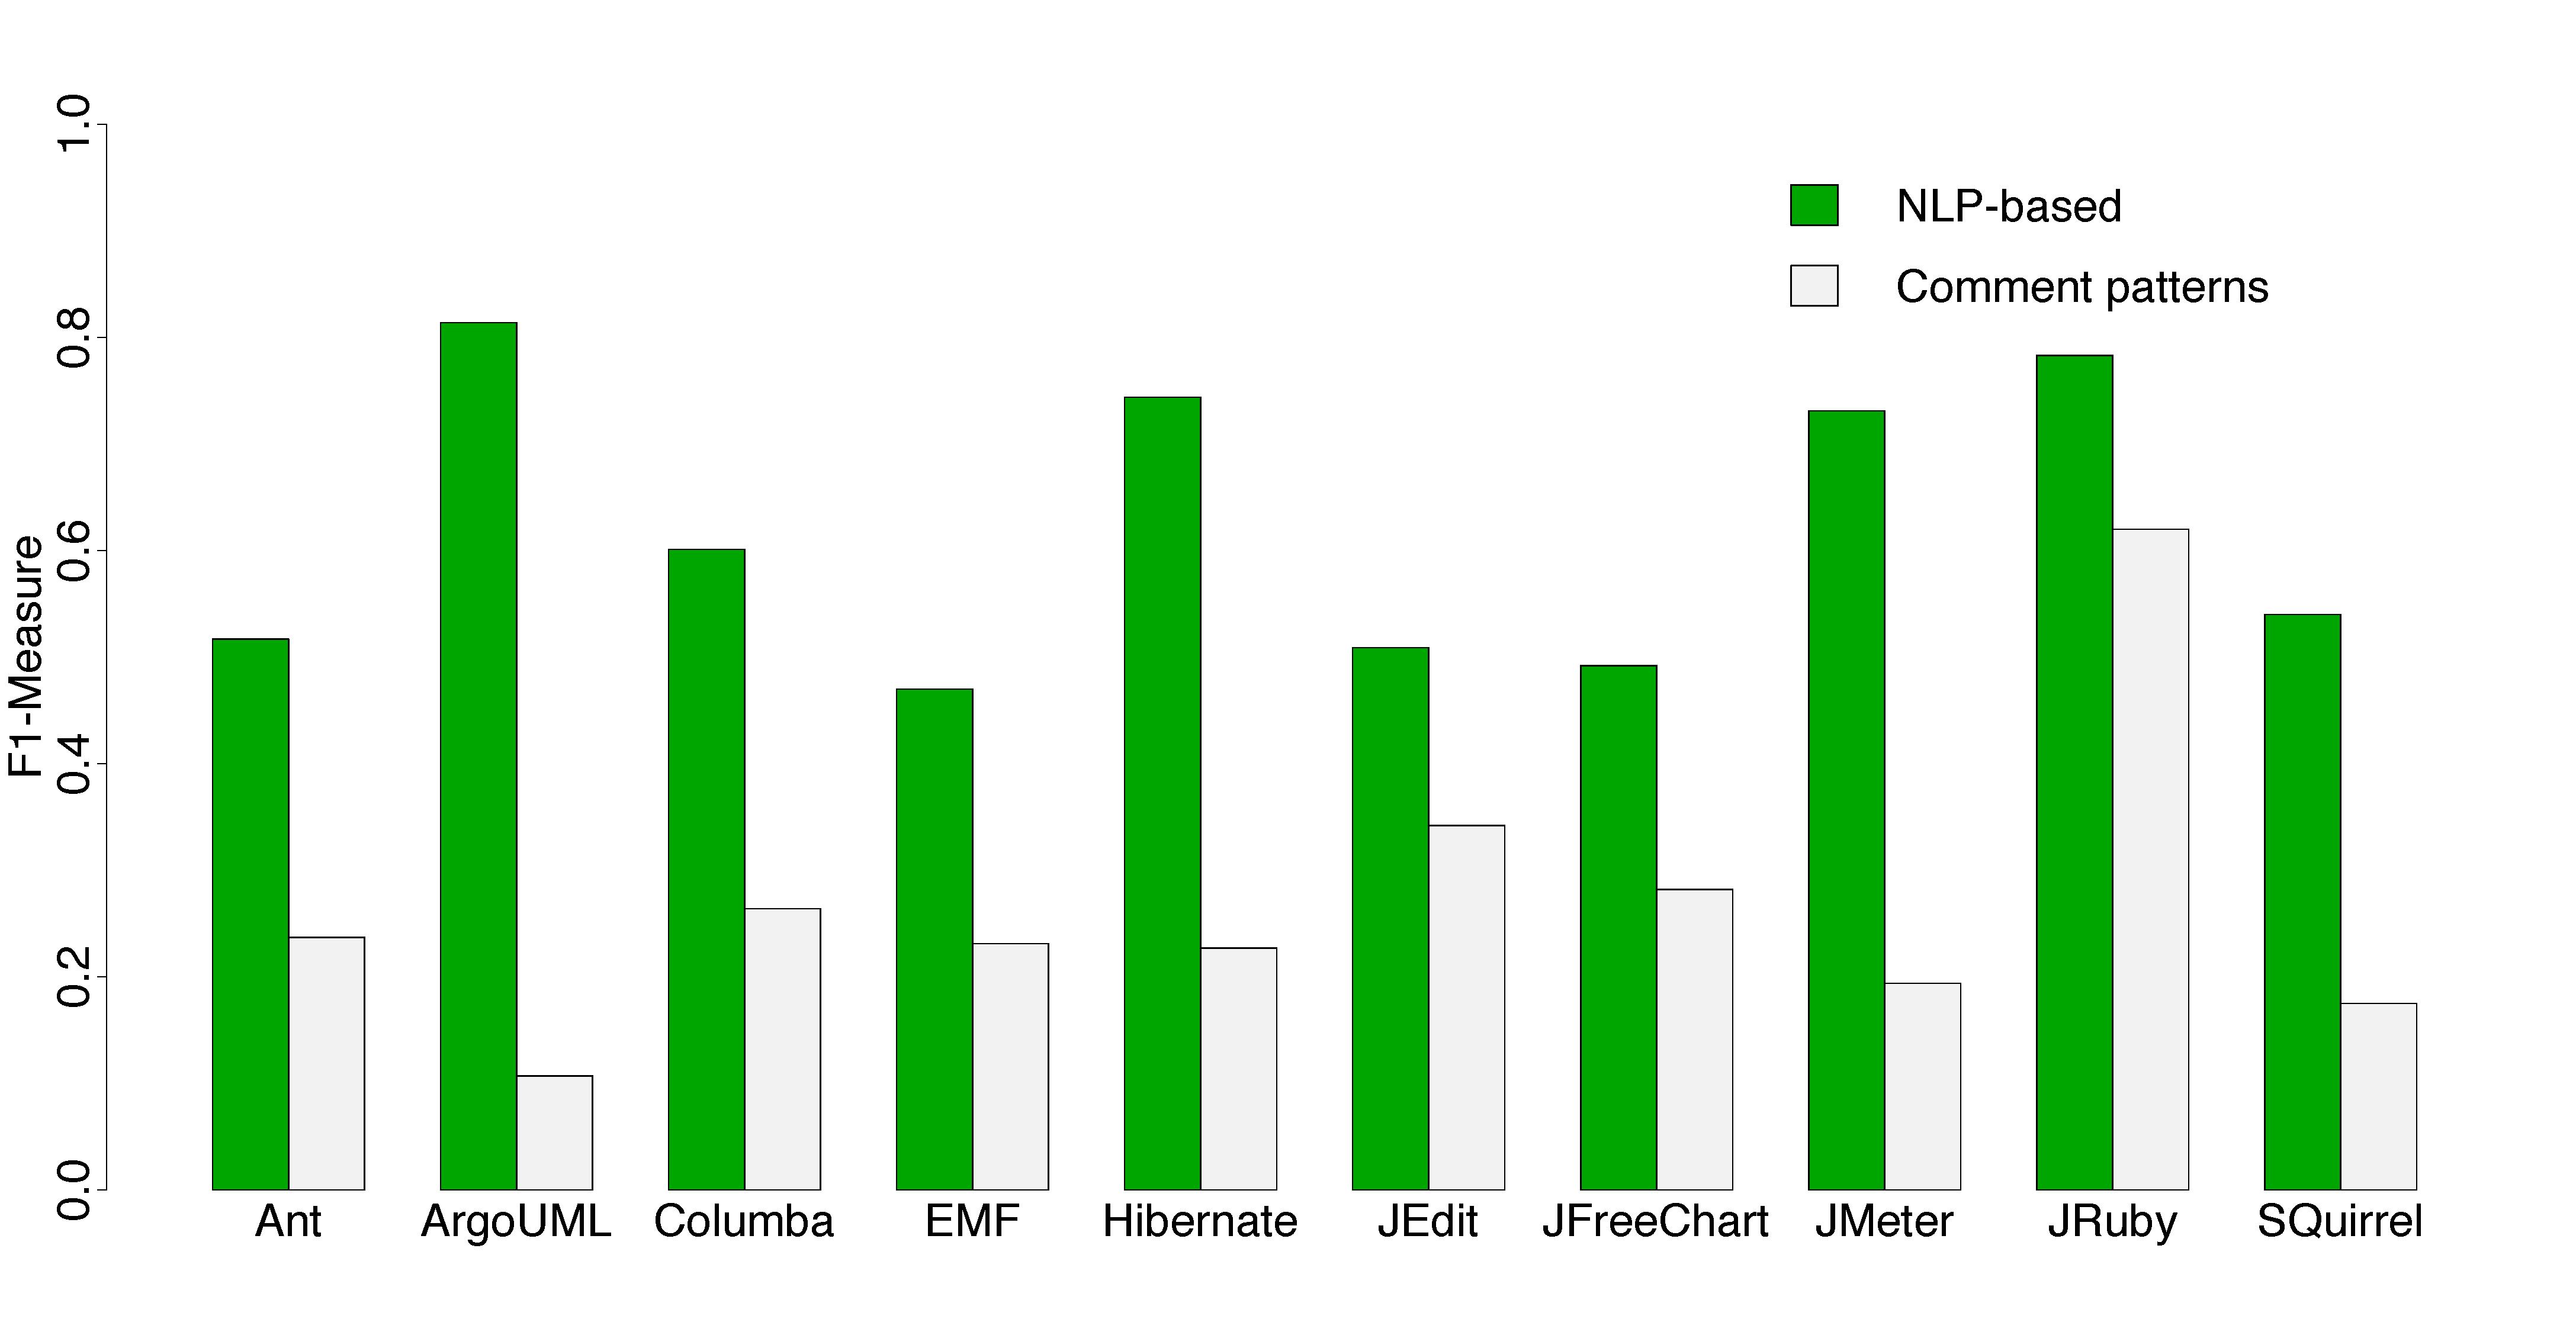
\includegraphics[width=.8\textwidth]{figures/chapter4/f1_measure_comparisom_design_2.pdf}
  \label{chap4:fig:f1_measure_comparison_design_debt}}
  \subfigure[Requirement Debt]{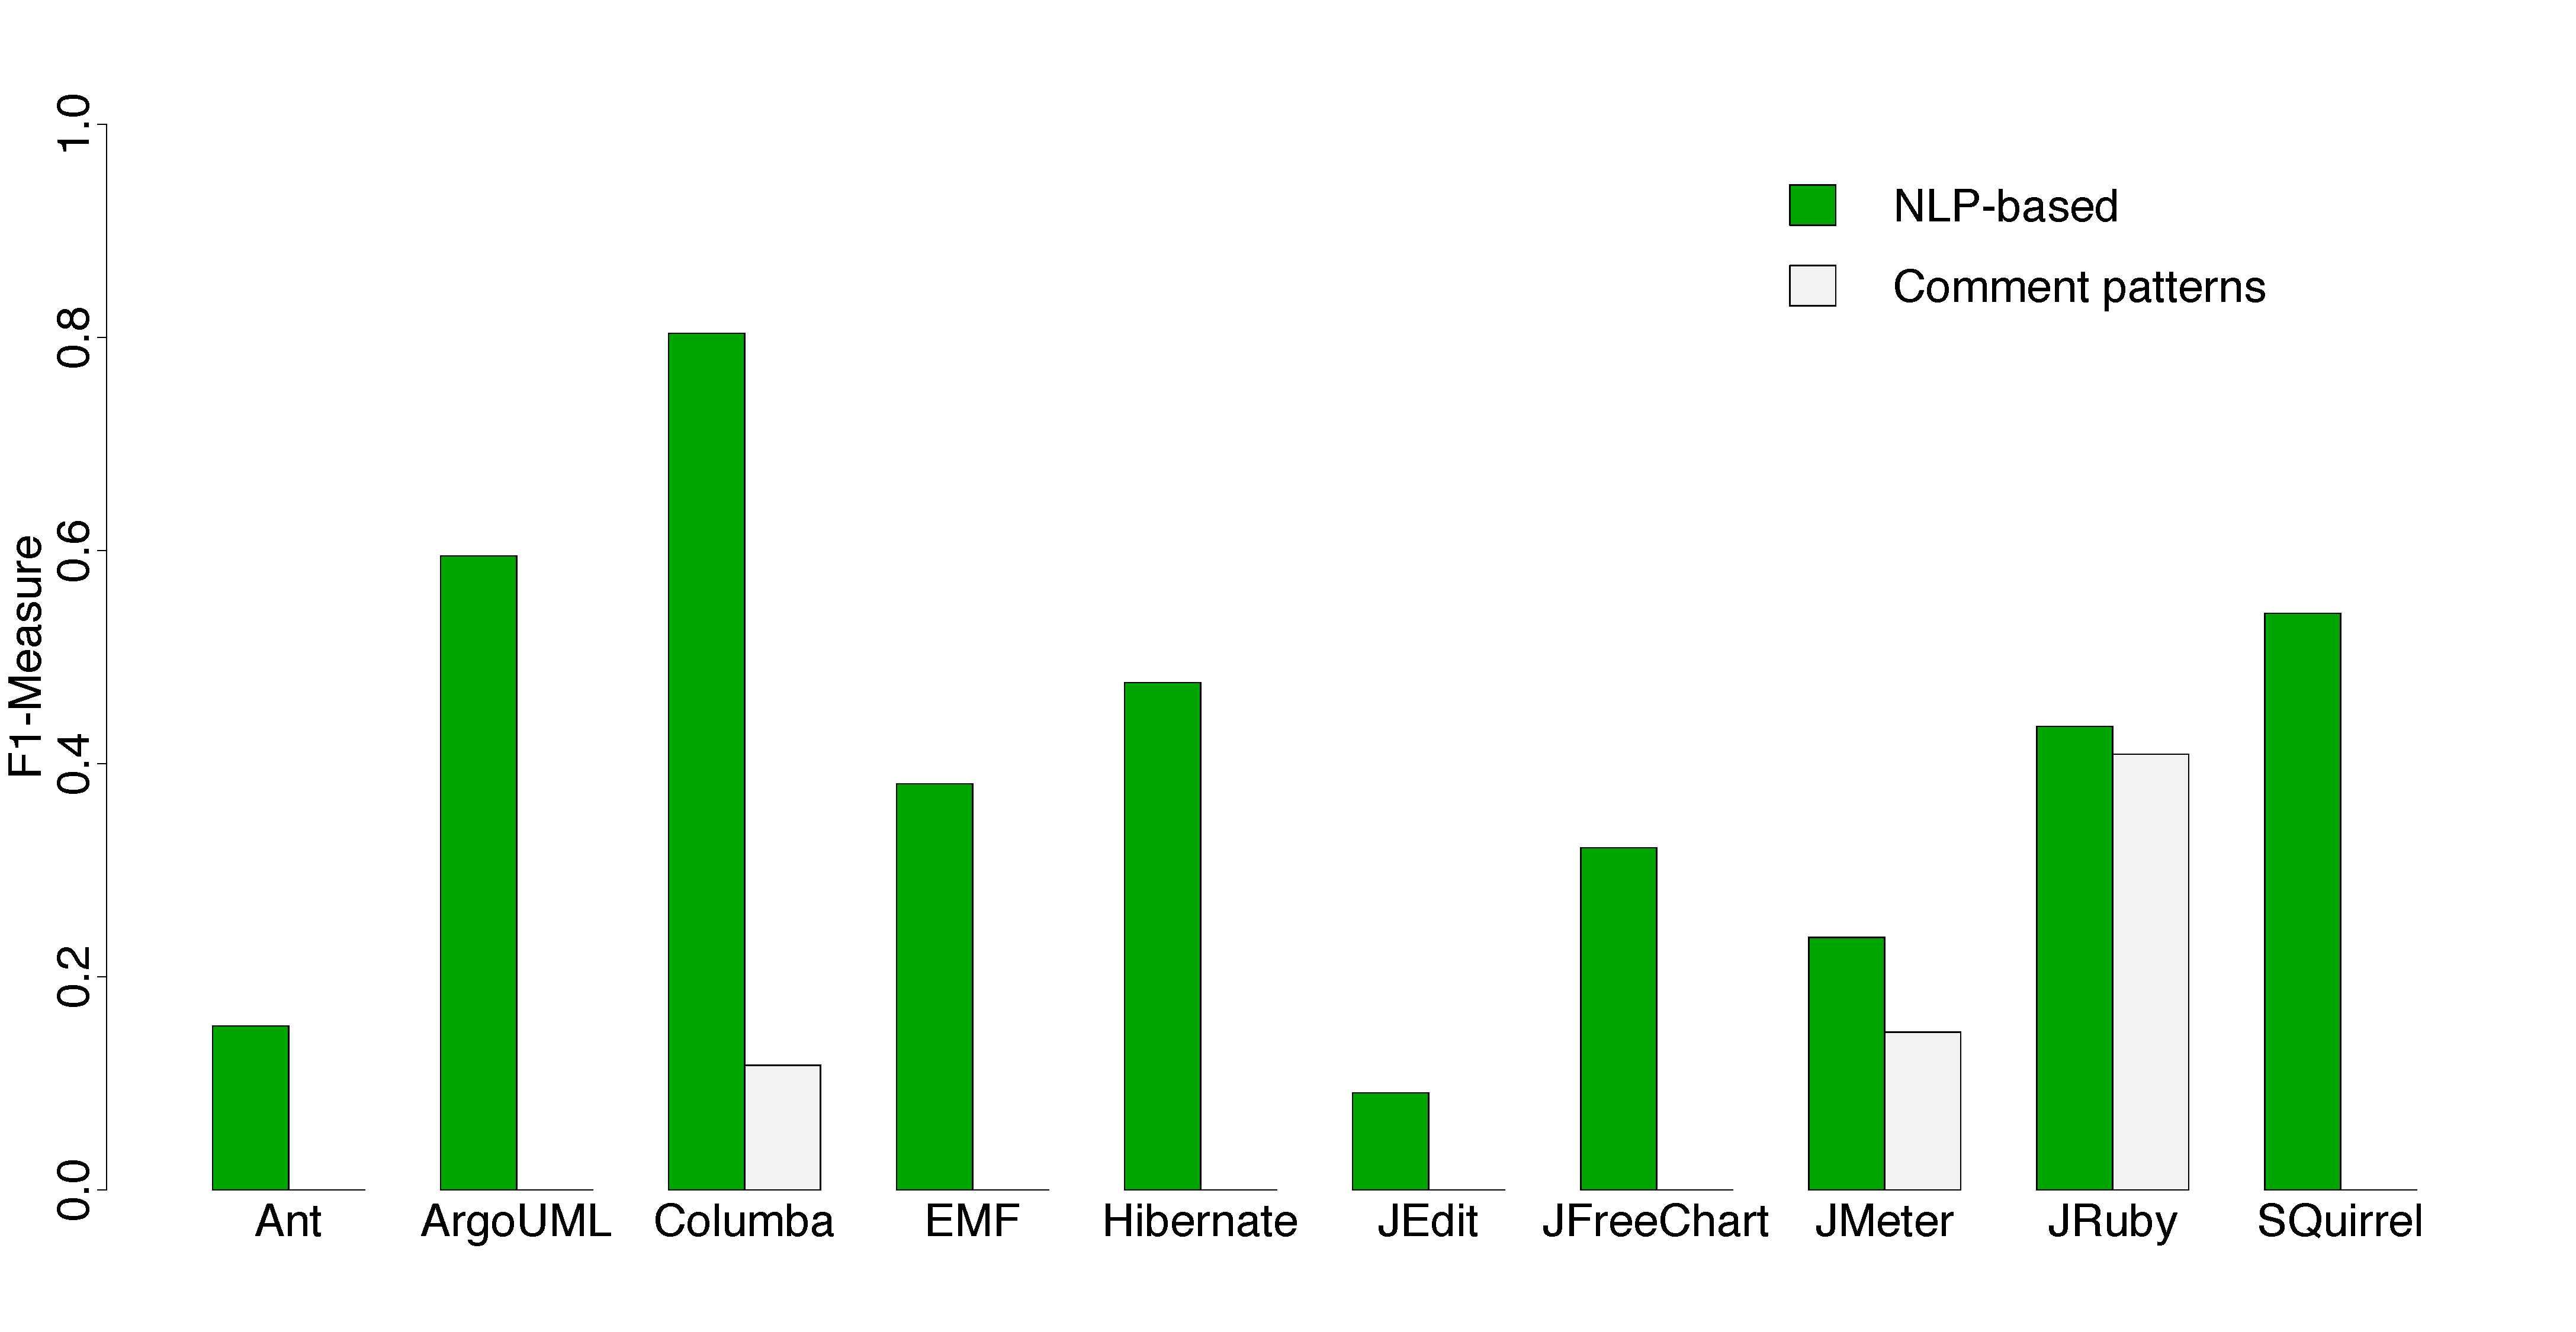
\includegraphics[width=.8\textwidth]{figures/chapter4/f1_measure_comparisom_requirement_2.pdf}
  \label{chap4:fig:f1_measure_comparison_requirement_debt}}
  
  \caption{Visualization of the F1-measure for Different Approaches}
\end{figure*}

\vspace{3mm}
\noindent\chapterIVrqi
\vspace{3mm}

\noindent \textbf{Motivation:} As shown in previous work~\cite{Maldonado2015MTD}, \SATD comments can be found in the source code. However, there is no automatic way to identify these comments. The methods proposed so far heavily rely on the manual inspection of source code, and there is no evidence on how well these approaches perform. Moreover, most of them do not discriminate between the different types of technical debt (e.g., design, test, requirement).

Therefore, we want to determine if NLP techniques such as, the maximum entropy classifier, can help us surpass these limitations and outperform the accuracy of the current state-of-the-art. The maximum entropy classifier can automatically classify comments based on specific linguistic characteristics of these comments. Answering this question is important, since it helps us understand the opportunities and limitations of using NLP techniques to automatically identify \SATD comments. 

\vspace{1mm}
\noindent \textbf{Approach:} For this research question, we would like to examine how effectively we can identify design and requirement \SATD. Therefore, the first step is to create a dataset that we can train and test the maximum entropy classifier on. We classified the source code comments into the following types of \SATD: design, defect, documentation, requirement, and test debt. However, our previous work showed that the most frequent \SATD comments are design and requirement debt. Therefore, in this paper, we focus on the identification of these two types of \SATD, because 1) they are the most common types of technical debt, and 2) NLP-based techniques require sufficient data for training (i.e., they cannot build an accurate model with a small number of samples).

We train the maximum entropy classifier using our manually created dataset. The dataset contains comments with and without \SATD, and each comment has a classification (i.e., without technical debt, design debt, or requirement debt). Then, we add to the training dataset all comments classified as without technical debt and the comments classified as the specific type of \SATD that we want to identify (i.e., design or requirement debt). We use the comments from 9 out of the 10 projects that we analyzed to create the training dataset. The comments from the remaining one project are used to evaluate the classification performed by the maximum entropy classifier. We choose to create the training dataset using comments from 9 out of 10 projects, because we want to train the maximum entropy classifier with the most diverse data possible (i.e., comments from different domains of applications). However, we discuss the implications of using training datasets of different sizes in RQ3. We repeat this process for each one of the ten projects, each time training on the other 9 projects and testing on the remaining 1 project.

Based on the training dataset, the maximum entropy classifier will classify each comment in the test dataset. The resulting classification is compared with the manual classification provided in the test dataset. If a comment in the test dataset has the same manual classification as the classification suggested by the maximum entropy classifier, we will have a true positive (tp) or a true negative (tn). True positives are the cases where the maximum entropy classifier correctly identifies \SATD comments, and true negatives are comments without technical debt that are classified as being as such. Similarly, when the classification provided by the tool diverges from the manual classification provided in the test dataset, we have false positives or false negatives. False positives (fp) are comments classified as being \SATD when they are not, and false negatives (fn) are comments classified as without technical debt when they really are \SATD comments. Using the tp, tn, fp, and fn values, we are able to evaluate the performance of different detection approaches in terms of precision ($P=\frac{tp}{tp + fp}$), recall ($R=\frac{tp}{tp + fn}$) and F1-measure ($F=2 \times \frac{P \times R}{P + R}$). To determine how effective the NLP classification is, we compare its F1-measure values with the corresponding F1-measure values of the state-of-the-art approach. We use the F1-measure to compare the performance between the approaches as it is the harmonic mean of precision and recall. Using the F1-measure allows us to incorporate the trade-off between precision and recall and present one value that evaluates both measures.

The state-of-the-art approach in detecting \SATD comments~\cite{Potdar2014ICSME} uses 62 comment patterns (i.e., keywords and phrases) that were found as recurrent in \SATD comments during the manual inspection of 101,762 comments. 

\vspace{1mm}

\noindent \textbf{Results - design debt:} Table \ref{chap4:tbl:improvement_f1measure} presents the F1-measure of the two approaches, as well as the improvement achieved by our approach compared to the other approaches. We see that for all projects, the F1-measure achieved by our approach is higher than the other approach. The F1-measure values obtained by our NLP-based approach range between 0.470 - 0.814, with an average of 0.620. In comparison, the F1-measure values using the comment patterns range between 0.107 - 0.620, with an average of 0.267. Figure \ref{chap4:fig:f1_measure_comparison_design_debt} visualizes the comparison of the F1-measure values for our NLP-based approach and the comment patterns approach. We see from both, Table \ref{chap4:tbl:improvement_f1measure} and Figure \ref{chap4:fig:f1_measure_comparison_design_debt} that, on average, our approach outperforms the comment patterns approach by 2.3 times when identifying design \SATD.

It is important to note that the comment patterns approach has a high precision, but low recall, i.e., this approach points correctly to \SATD comments, but as it depends on keywords, it identifies a very small subset of all the \SATD comments in the project. Although we only show the F1-measure values here, we present the precision and recall values in Table~\ref{chap4:tbl:classifier_results_vs_baseline_design}.  

\noindent \textbf{Results - requirement debt:} Similarly, the last 3 columns of Table \ref{chap4:tbl:improvement_f1measure} show the F1-measure performance of the two approaches, and the improvement achieved by our approach over the other approaches. The comment patterns approach was able to identify requirement \SATD in only 3 of the 10 analyzed projects. A possible reason for the low performance of the comment patterns in detecting requirement debt is that the comment patterns do not differentiate between the different types of \SATD. Moreover, since most of the debt is design debt, it is possible that the patterns tend to favor the detection of design debt.
 
That said, we find that for all projects, the F1-measure values obtained by our approach surpass the F1-measure values of the other approach. Our approach achieves F1-measure values between 0.091 - 0.804 with an average of 0.403, whereas the comment pattern approach achieves F1-measure values in the range of 0.117 - 0.409 with an average of 0.067. Figure \ref{chap4:fig:f1_measure_comparison_requirement_debt} visualizes the performance comparison of the two approaches. We also examine if the differences in the F1-measure values obtained by our approach and the other baseline are statistically significant. Indeed, we find that the differences are statistically significant (p\textless0.001) for both design and requirement \SATD.

Generally, requirement \SATD is less common than design \SATD, which makes it more difficult to detect. Nevertheless, our NLP-based approach provides a significant improvement over the comment patterns approach, outperforming it by 6 times, on average. Table~\ref{chap4:tbl:improvement_f1measure} only presents the F1-measure values for the sake of brevity, however, we present the detailed precision and recall values in Table \ref{chap4:tbl:classifier_results_vs_baseline_requirement}.

% \subsection{Investigating the Impact of Different Classifiers on the Accuracy of the Classification}
% \label{chap4:sec:underlying_classifier}
In our work, the classification performed by the Stanford Classifier used the maximum entropy classifier. However, the Stanford Classifier can use other classifiers too. In order to examine the impact of the underlying classifier on the accuracy of the proposed approach, we investigate two more classifiers, namely the Naive Bayes, and the Binary classifiers.
 
Figures~\ref{chap4:fig:algorithms_comparison_design} and \ref{chap4:fig:algorithms_comparison_requirement} compare the performance between the three different classifiers. We find that the Naive Bayes has the worst average F1-measure of 0.30 and 0.05 for design and requirement technical debt, respectively. Based on our findings, the Naive Bayes algorithm favours recall at the expense of precision. For example, while classifying design debt, the average recall was 0.84 and precision 0.19. The two other algorithms present more balanced results compared to the Naive Bayes, and the difference in their performance is almost negligible. The Logistic Regression classifier achieved F1-measures of 0.62 and 0.40, while the Binary classifier F1-measures were 0.63 and 0.40, for design and requirement \SATD, respectively. Tables \ref{chap4:tbl:improvement_f1measure_between_classifiers_design} and \ref{chap4:tbl:improvement_f1measure_between_classifiers_requirement} provide detailed data for each classifier and all ten examined projects.

Although the Binary classifier has a slightly better performance, for our purpose, the Logistical Regression classifier provides more insightful textual features. These features were analyzed and presented in RQ2. 

According to previous work, developers hate to deal with false positives (i.e., low precision) \cite{Bessey2010FBL,Ernst2015FSE,Sadowski2015ICSE}. Due to this fact, we choose to present our results in this study using the maximum entropy classifier, which has an average precision of 0.716 throughout all projects. However, favouring recall over precision by using the Naives Bayes classifier might still be acceptable, if a manual process to filter out false positives is in place, as reported by Berry et al. \cite{Berry2012book}.

One important question to ask when choosing what kind of classifier to use is how much training data is currently available. In most of the cases, the trickiest part of applying a machine learning classifier in real world applications is creating or obtaining enough training data. If you have fairly little data at your disposal, and you are going to train a supervised classifier, then machine learning theory recommends classifiers with high bias, such as the Naive Bayes~\cite{Forman2004PKDD,Ng2001NIPS}. If there is a reasonable amount of labeled data, then you are in good stand to use most kinds of classifiers~\cite{Manning2008book}. For instance, you may wish to use a Support Vector Machine (SVM), a decision tree or, like in our study, a max entropy classifier. If a large amount of data is available, then the choice of classifier probably has little effect on the results and the best choice may be unclear~\cite{Banko2001book}. It may be best to choose a classifier based on the scalability of training, or even runtime efficiency.

\begin{landscape}
\begin{table}[h]
  
    \centering
        \caption{Comparison Between Different Classifiers for Design Debt}
        
        \label{chap4:tbl:improvement_f1measure_between_classifiers_design}
        \resizebox{\columnwidth}{!}{%
        \begin{tabular}{l| c c c|| c c c|| c c c }
        \toprule

        \multirow{4}{*}{\textbf{\thead{Project}}} & \multicolumn{3}{c||}{\textbf{\thead{Maximum Entropy}}} & \multicolumn{3}{c||}{\textbf{\thead{Naive Bayes}}} & \multicolumn{3}{c}{\textbf{\thead{Binary}}} 
        
        \\ 
        \cmidrule{2-10}
        
        & \textbf{\thead{Precision}} & \textbf{\thead{Recall}} & \textbf{\thead{F1 measure}} & \textbf{\thead{Precision}} & \textbf{\thead{Recall}} & \textbf{\thead{F1 measure}} & \textbf{\thead{Precision}} & \textbf{\thead{Recall}} & \textbf{\thead{F1 measure}}\\
        \midrule                                                  
        \textbf{Ant}          &  0.554 & 0.484 &  0.517 &  0.072 & 0.874 & 0.134 &  0.620 & 0.516 & 0.563  \\
        \textbf{ArgoUML}      &  0.788 & 0.843 &  0.814 &  0.358 & 0.985 & 0.525 &  0.790 & 0.858 & 0.822  \\
        \textbf{Columba}      &  0.792 & 0.484 &  0.601 &  0.181 & 0.786 & 0.294 &  0.840 & 0.500 & 0.627  \\
        \textbf{EMF}          &  0.574 & 0.397 &  0.470 &  0.057 & 0.872 & 0.106 &  0.633 & 0.397 & 0.488  \\
        \textbf{Hibernate}    &  0.877 & 0.645 &  0.744 &  0.288 & 0.890 & 0.435 &  0.895 & 0.670 & 0.767  \\
        \textbf{JEdit}        &  0.779 & 0.378 &  0.509 &  0.227 & 0.791 & 0.353 &  0.807 & 0.342 & 0.480  \\
        \textbf{JFreeChart}   &  0.646 & 0.397 &  0.492 &  0.140 & 0.560 & 0.224 &  0.658 & 0.397 & 0.495  \\
        \textbf{JMeter}       &  0.808 & 0.668 &  0.731 &  0.224 & 0.801 & 0.350 &  0.819 & 0.671 & 0.737  \\
        \textbf{JRuby}        &  0.798 & 0.770 &  0.783 &  0.275 & 0.971 & 0.429 &  0.815 & 0.808 & 0.811  \\
        \textbf{SQuirrel}     &  0.544 & 0.536 &  0.540 &  0.133 & 0.947 & 0.233 &  0.567 & 0.550 & 0.558  \\
        \midrule                                                  
        \textbf{Average}      &  0.716 &   0.5602 &  0.6201 &  0.1955  & 0.8477  & 0.3083 & 0.7444  & 0.5709 & 0.6348  \\
        \bottomrule
        \end{tabular}}    
\end{table}
\end{landscape}

\begin{landscape}
\begin{table}[h]
  
    \centering
        \caption{Comparison Between Different Classifiers for Requirement Debt}
        
        \label{chap4:tbl:improvement_f1measure_between_classifiers_requirement}
        \resizebox{\columnwidth}{!}{%
        \begin{tabular}{l| c c c|| c c c|| c c c }
        \toprule
        \multirow{4}{*}{\textbf{\thead{Project}}} & \multicolumn{3}{c||}{\textbf{\thead{Maximum Entropy}}} & \multicolumn{3}{c||}{\textbf{\thead{Naive Bayes}}} & \multicolumn{3}{c}{\textbf{\thead{Binary}}} 
        
        \\ 
        \cmidrule{2-10}
        
        & \textbf{\thead{Precision}} & \textbf{\thead{Recall}} & \textbf{\thead{F1 measure}} & \textbf{\thead{Precision}} & \textbf{\thead{Recall}} & \textbf{\thead{F1 measure}} & \textbf{\thead{Precision}} & \textbf{\thead{Recall}} & \textbf{\thead{F1 measure}}\\
        \midrule                                                  
        \textbf{Ant}          &  0.154 & 0.154 & 0.154 & 0.007 &  0.769 & 0.013 & 0.188 & 0.231 & 0.207 \\
        \textbf{ArgoUML}      &  0.663 & 0.540 & 0.595 & 0.119 &  0.808 & 0.207 & 0.659 & 0.569 & 0.611 \\
        \textbf{Columba}      &  0.755 & 0.860 & 0.804 & 0.030 &  0.930 & 0.057 & 0.755 & 0.860 & 0.804 \\
        \textbf{EMF}          &  0.800 & 0.250 & 0.381 & 0.009 &  1.000 & 0.018 & 0.800 & 0.250 & 0.381 \\
        \textbf{Hibernate}    &  0.610 & 0.391 & 0.476 & 0.041 &  0.781 & 0.078 & 0.615 & 0.375 & 0.466 \\
        \textbf{JEdit}        &  0.125 & 0.071 & 0.091 & 0.011 &  0.857 & 0.022 & 0.143 & 0.071 & 0.095 \\
        \textbf{JFreeChart}   &  0.220 & 0.600 & 0.321 & 0.009 &  0.800 & 0.018 & 0.179 & 0.467 & 0.259 \\
        \textbf{JMeter}       &  0.153 & 0.524 & 0.237 & 0.011 &  0.952 & 0.022 & 0.180 & 0.524 & 0.268 \\
        \textbf{JRuby}        &  0.686 & 0.318 & 0.435 & 0.058 &  0.836 & 0.109 & 0.679 & 0.327 & 0.442 \\
        \textbf{SQuirrel}     &  0.657 & 0.460 & 0.541 & 0.018 &  0.900 & 0.036 & 0.455 & 0.500 & 0.476 \\
        \midrule                                                  
        \textbf{Average}      & 0.4823 &  0.4168 & 0.4035 & 0.0313 & 0.8633 & 0.058  & 0.4653 & 0.4174 & 0.4009 \\
        \bottomrule
        \end{tabular}}    
\end{table} 
\end{landscape}

\clearpage
\begin{figure*}[!thb]
  \centering
  \subfigure[Design Debt]{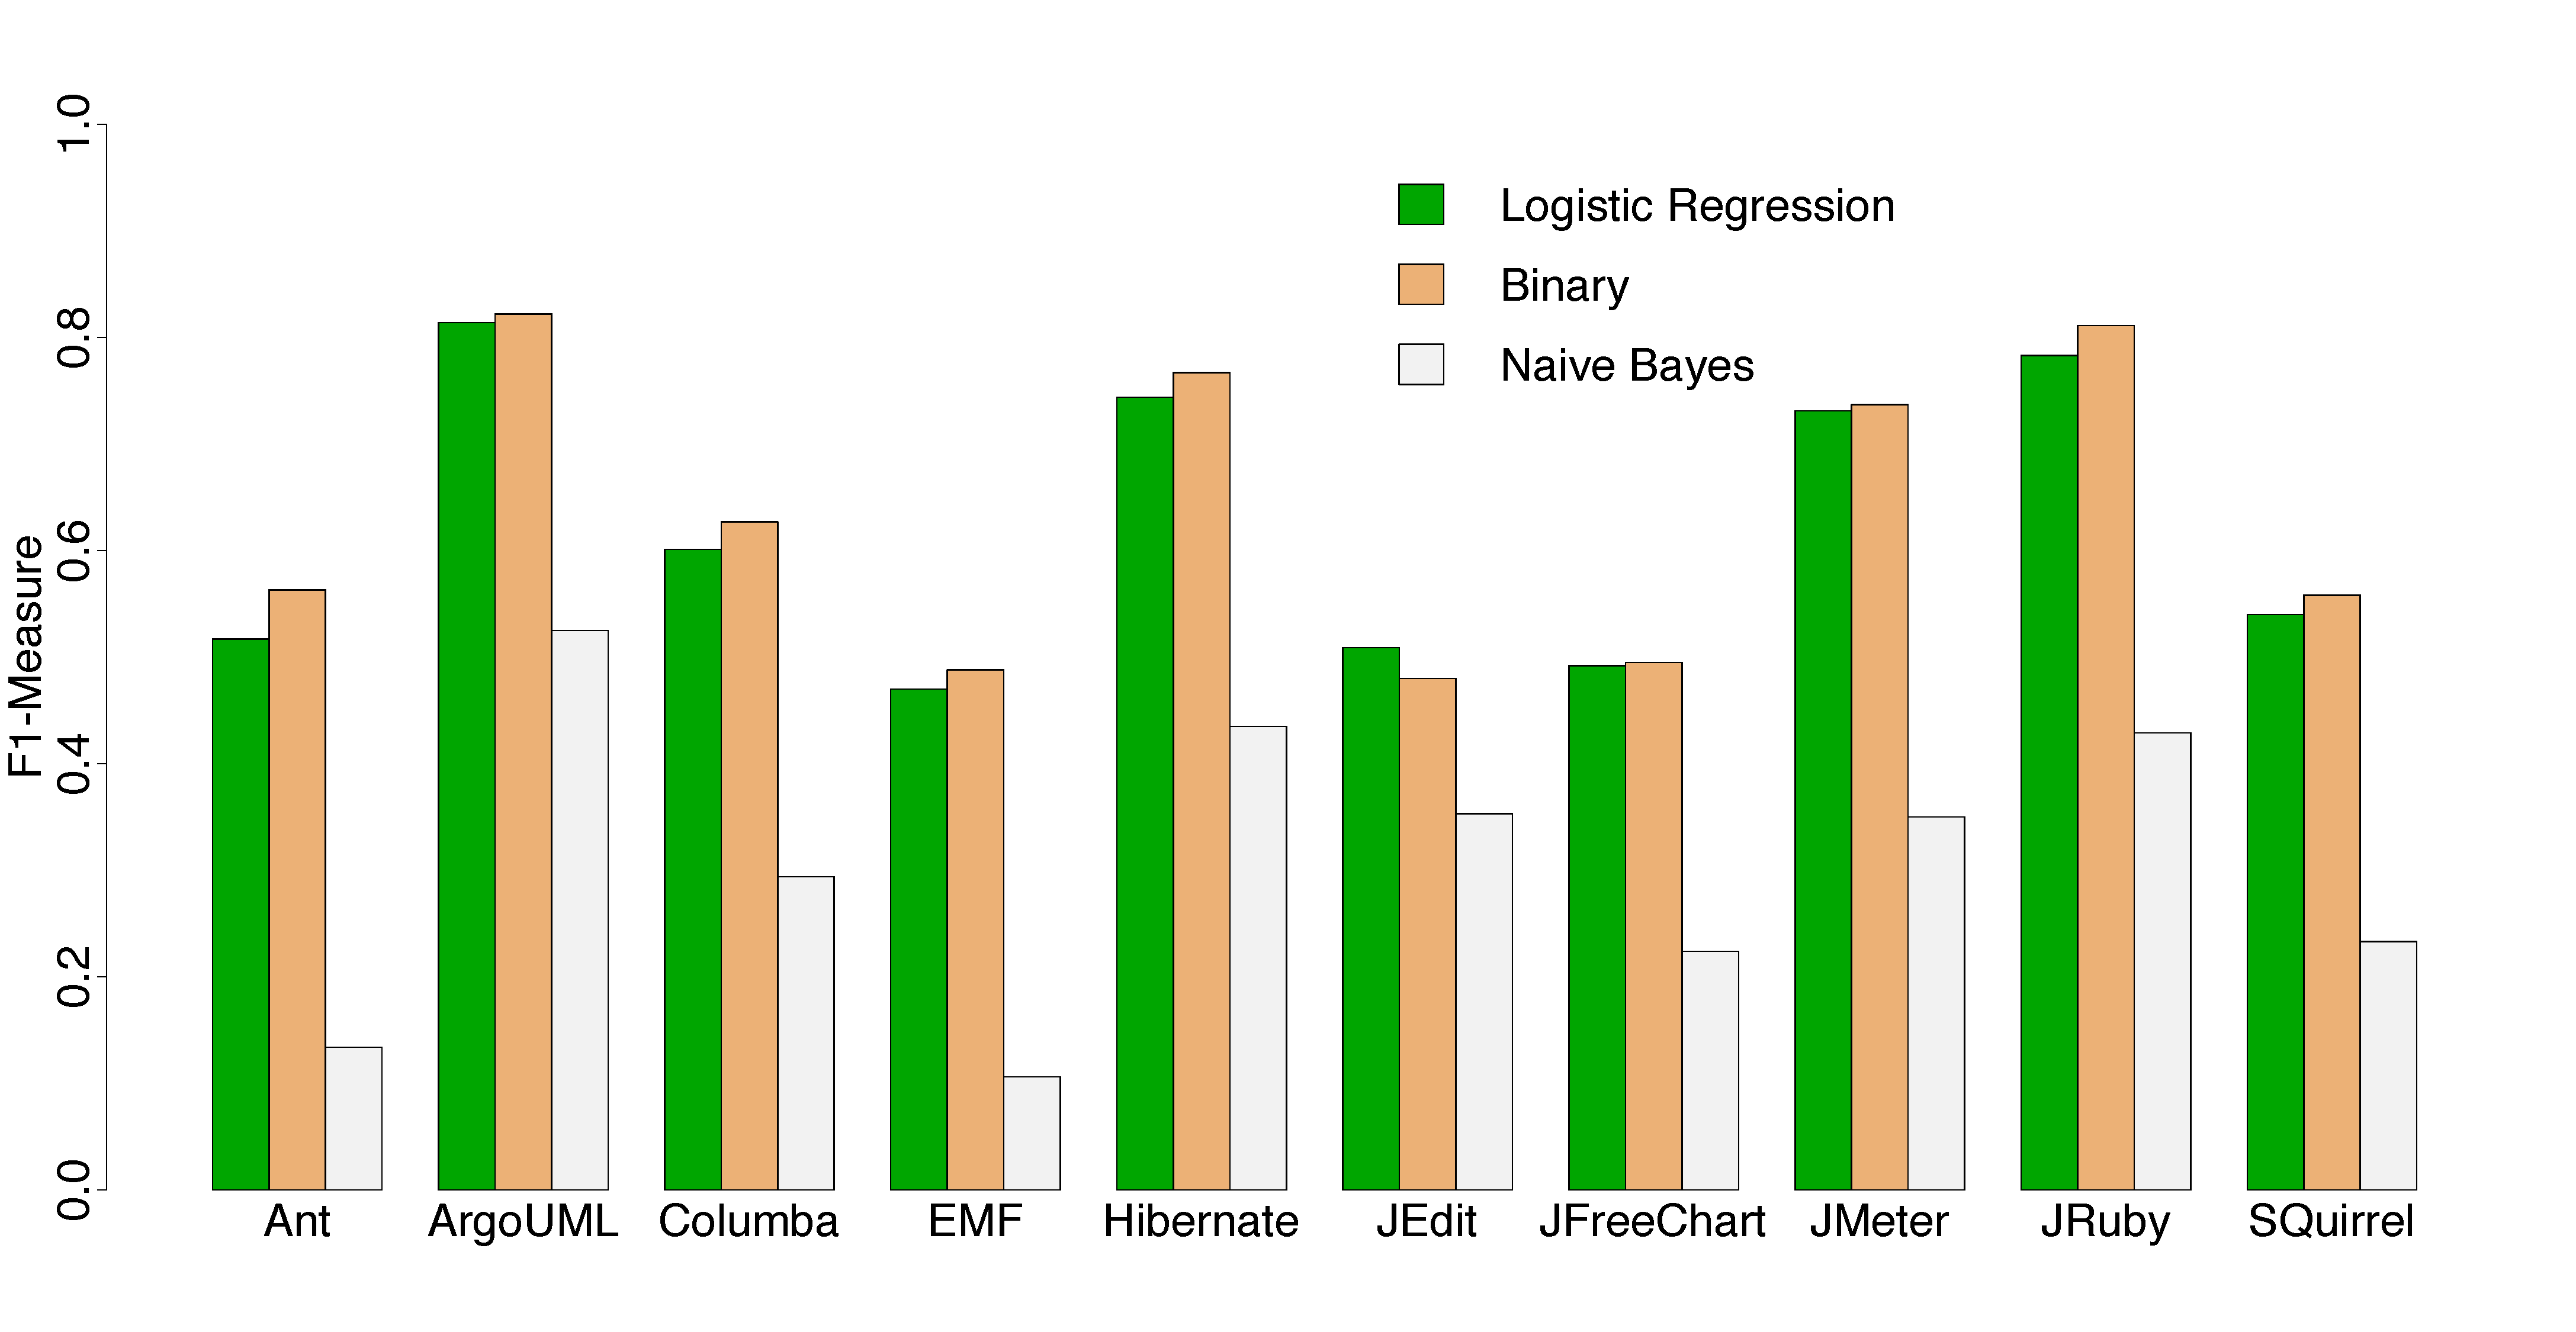
\includegraphics[width=0.8\textwidth]{figures/chapter4/classifier_algorithms_comparison_design_1.pdf}
  \label{chap4:fig:algorithms_comparison_design}}
  \subfigure[Requirement Debt]{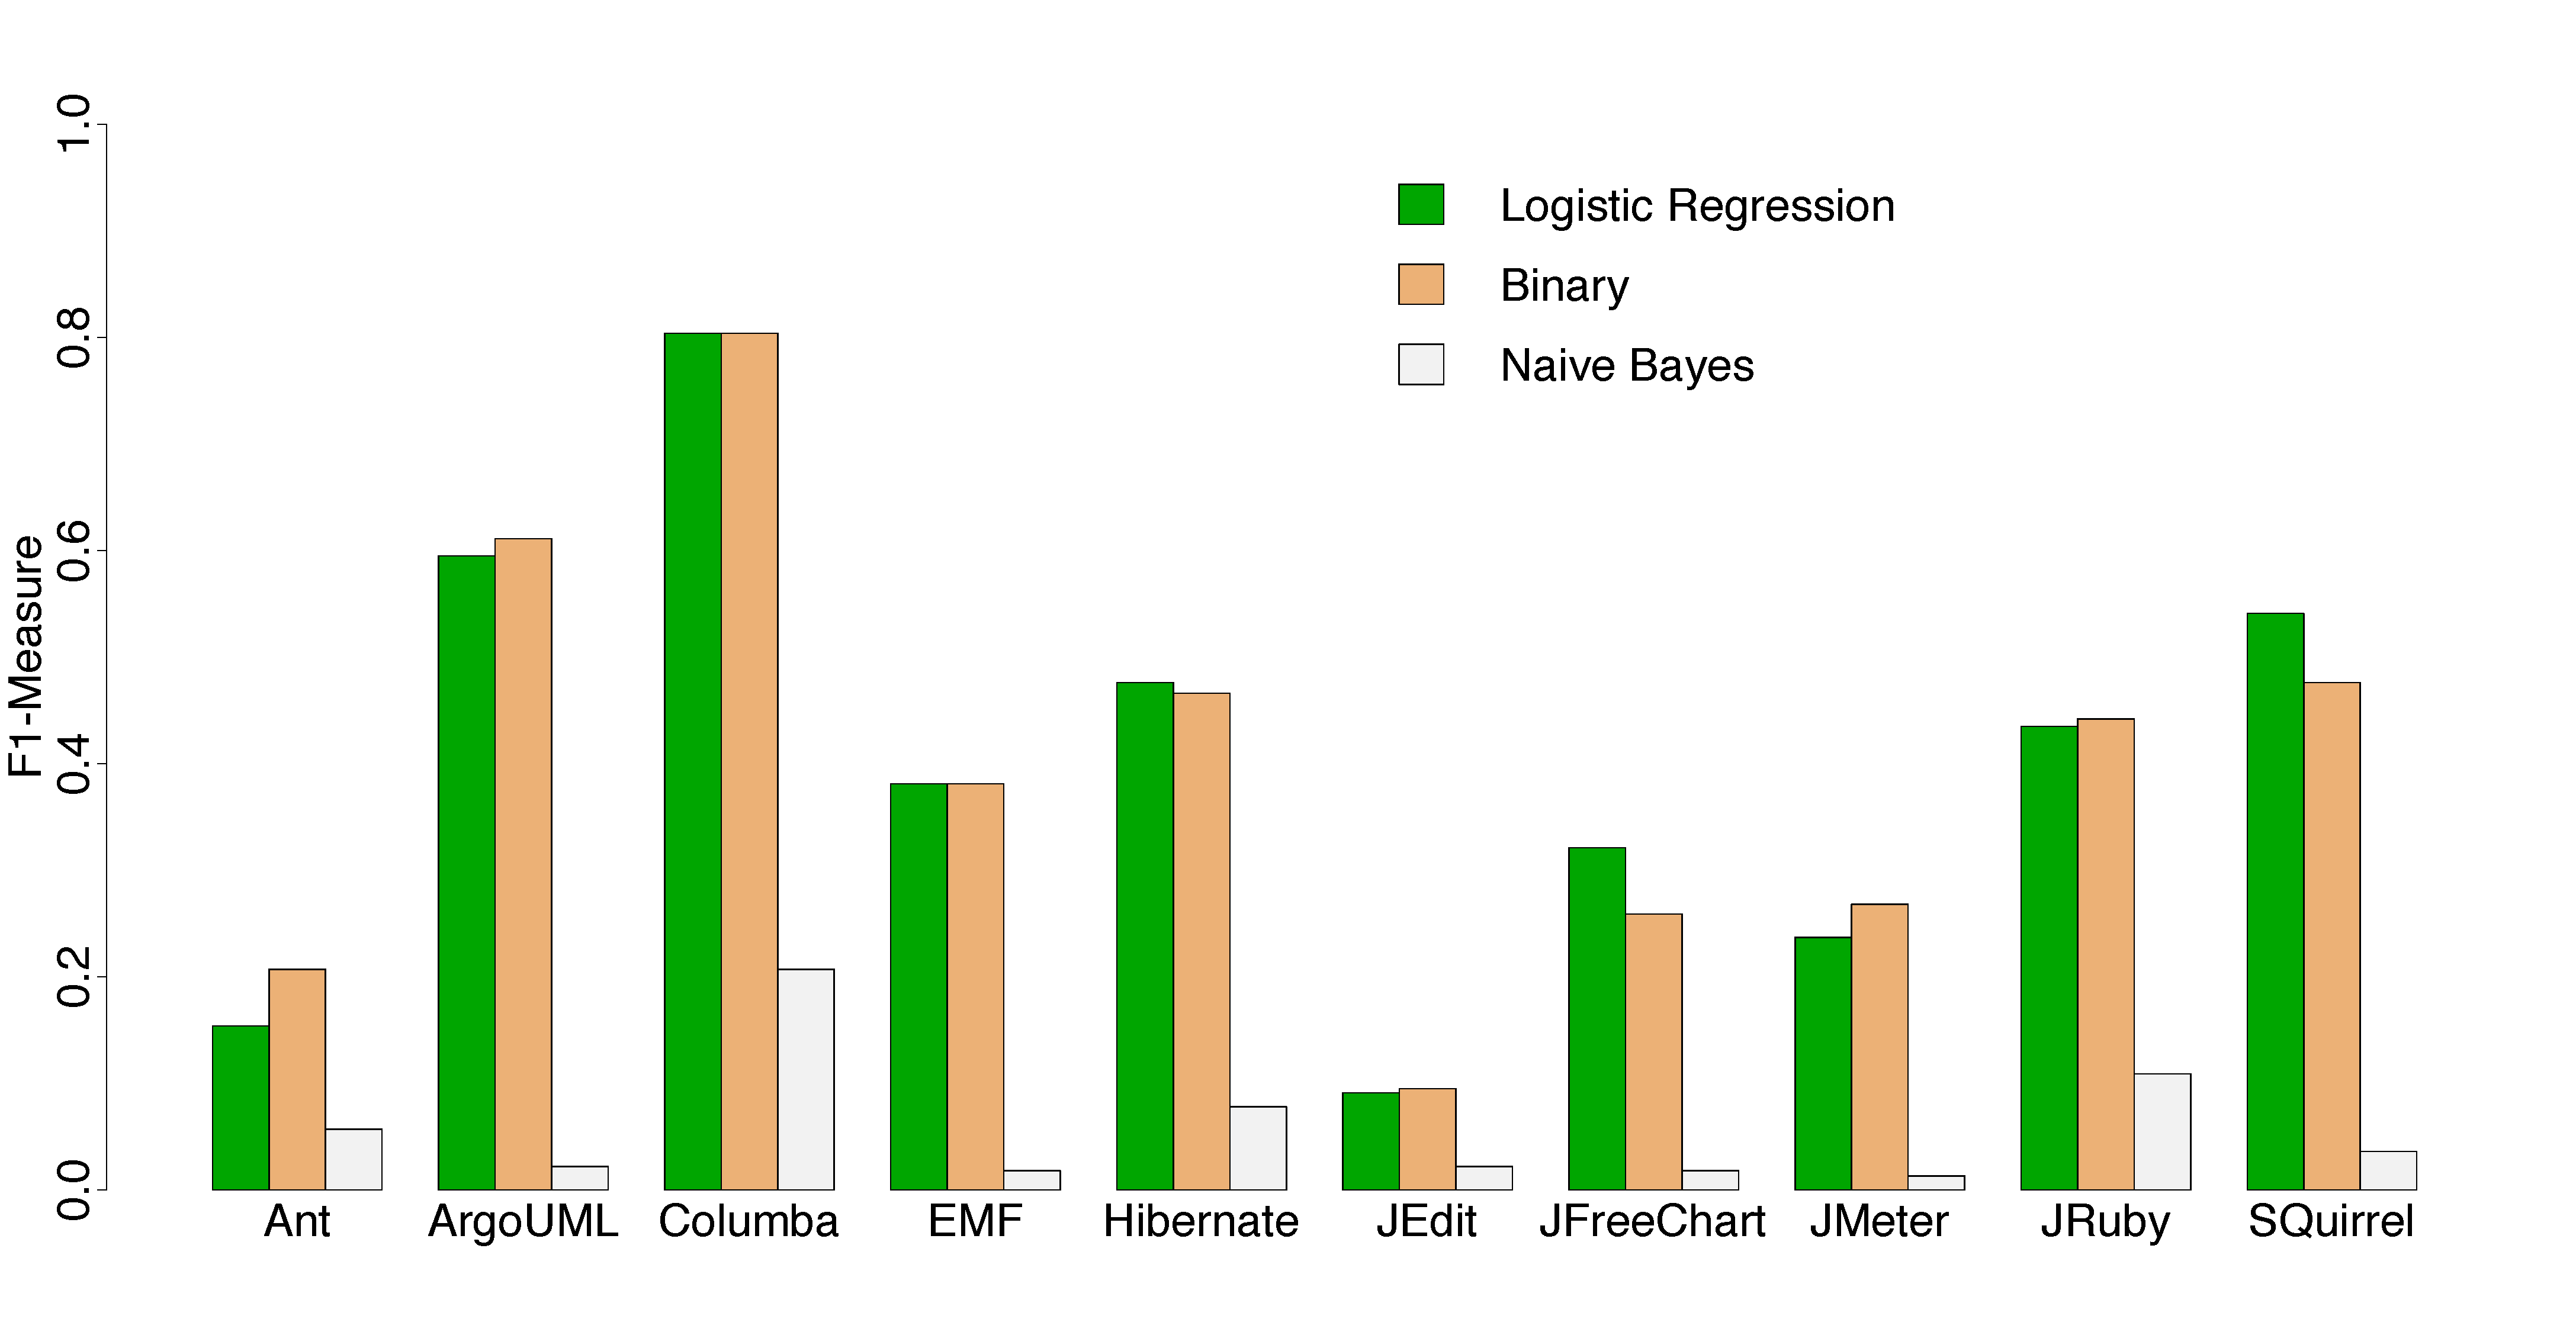
\includegraphics[width=0.8\textwidth]{figures/chapter4/classifier_algorithms_comparison_implementation_1.pdf}
  \label{chap4:fig:algorithms_comparison_requirement}}
  \caption{Underlying Classifier Algorithms Performance Comparison}
  \label{chap4:fig:algorithms_comparison}
\end{figure*}


\conclusionbox{We find that our NLP-based approach, is more accurate in identifying self-admitted technical debt comments compared to the current state-of-art. We achieved an average F1-measure of 0.620 when identifying design debt (an average improvement of 2.3$\times$ over the state-of-the-art approach) and an average F1-measure of 0.403 when identifying requirement debt (an average improvement of 6$\times$ over the state-of-the-art approach).}

\begin{landscape}
\begin{table}[h]
  
    \centering
        \caption{Detailed Comparison of F1-measure Between the NLP-based and the Comment Patterns Approach for Design Debt}
        
        \label{chap4:tbl:classifier_results_vs_baseline_design}
        \resizebox{\columnwidth}{!}{%
        \begin{tabular}{l| c c c|| c c c}
        \toprule

        \multirow{4}{*}{\textbf{\thead{Project}}} & \multicolumn{3}{c||}{\textbf{\thead{NLP-based}}} & \multicolumn{3}{c}{\textbf{\thead{Comment Patterns}}} 
        
        \\ 
        \cmidrule{2-7}
        
        & \textbf{\thead{Precision}} & \textbf{\thead{Recall}} & \textbf{\thead{F1 measure}} & \textbf{\thead{Precision}} & \textbf{\thead{Recall}} & \textbf{\thead{F1 measure}} \\
        \midrule
        \textbf{Ant}           &   0.554 &   0.484 &  0.517 &  0.608 & 0.147 & 0.237  \\
        \textbf{ArgoUML}       &   0.788 &   0.843 &  0.814 &  0.793 & 0.057 & 0.107  \\
        \textbf{Columba}       &   0.792 &   0.484 &  0.601 &  0.800 & 0.158 & 0.264  \\
        \textbf{EMF}           &   0.574 &   0.397 &  0.470 &  0.647 & 0.141 & 0.231  \\
        \textbf{Hibernate}     &   0.877 &   0.645 &  0.744 &  0.920 & 0.129 & 0.227  \\
        \textbf{JEdit}         &   0.779 &   0.378 &  0.509 &  0.857 & 0.214 & 0.342  \\
        \textbf{JFreeChart}    &   0.646 &   0.397 &  0.492 &  0.507 & 0.195 & 0.282  \\
        \textbf{JMeter}        &   0.808 &   0.668 &  0.731 &  0.813 & 0.110 & 0.194  \\
        \textbf{JRuby}         &   0.798 &   0.770 &  0.783 &  0.864 & 0.483 & 0.620  \\
        \textbf{SQuirrel}      &   0.544 &   0.536 &  0.540 &  0.700 & 0.100 & 0.175  \\
        \bottomrule
        \end{tabular}}
\end{table}
\end{landscape}                 

\begin{landscape}
\begin{table}[h]
  
    \centering
        \caption{Detailed Comparison of F1-measure Between the NLP-based and the Comment Patterns Approach for Requirement Debt}
        
        \label{chap4:tbl:classifier_results_vs_baseline_requirement}
        \resizebox{\columnwidth}{!}{%
        \begin{tabular}{l| c c c|| c c c}
        \toprule

        \multirow{4}{*}{\textbf{\thead{Project}}} & \multicolumn{3}{c||}{\textbf{\thead{NLP-based}}} & \multicolumn{3}{c}{\textbf{\thead{Comment Patterns}}} 
        
        \\ 
        \cmidrule{2-7}
        
        & \textbf{\thead{Precision}} & \textbf{\thead{Recall}} & \textbf{\thead{F1 measure}} & \textbf{\thead{Precision}} & \textbf{\thead{Recall}} & \textbf{\thead{F1 measure}} \\
        \midrule
        \textbf{Ant}           &  0.154 & 0.154 &  0.154 & 0.000  &  0.000   & 0.000  \\
        \textbf{ArgoUML}       &  0.663 & 0.540 &  0.595 & 0.000  &  0.000   & 0.000  \\
        \textbf{Columba}       &  0.755 & 0.860 &  0.804 & 0.375  &  0.069   & 0.117  \\
        \textbf{EMF}           &  0.800 & 0.250 &  0.381 & 0.000  &  0.000   & 0.000  \\
        \textbf{Hibernate}     &  0.610 & 0.391 &  0.476 & 0.000  &  0.000   & 0.000  \\
        \textbf{JEdit}         &  0.125 & 0.071 &  0.091 & 0.000  &  0.000   & 0.000  \\
        \textbf{JFreeChart}    &  0.220 & 0.600 &  0.321 & 0.102  &  0.266   & 0.148  \\
        \textbf{JMeter}        &  0.153 & 0.524 &  0.237 & 0.000  &  0.000   & 0.000  \\
        \textbf{JRuby}         &  0.686 & 0.318 &  0.435 & 0.573  &  0.318   & 0.409  \\
        \textbf{SQuirrel}      &  0.657 & 0.460 &  0.541 & 0.000  &  0.000   & 0.000  \\
        \bottomrule
        \end{tabular}}   
\end{table}
\end{landscape}

\vspace{3mm}
\noindent\chapterIVrqii
\vspace{3mm}

\noindent \textbf{Motivation:} After assessing the accuracy of our NLP-based approach in identifying \SATD comments, we want to better understand what words developers use when expressing technical debt. Answering this question will provide insightful information that can guide future research directions, broaden our understanding on \SATD and also help us to detect it.     

\vspace{1mm}
\noindent \textbf{Approach:} The maximum entropy classifier learns optimal features that can be used to detect \SATD. A feature is comment fragment (e.g., word) that is associated with a specific class (i.e., design debt, requirement debt, or without technical debt), and a weight that represents how strongly this feature relates to that class. The maximum entropy classifier uses the classified training data to determine the features and their weights. Then, these features and their corresponding weights are used to determine if a comment belongs to a specific type of \SATD or not.

For example, let us assume that after the training, the maximum entropy classifier determines that the features ``hack'' and ``dirty'' are related to the \textit{design-debt} class with weights 5.3 and 3.2, respectively, and the feature ``something'' relates to the \textit{without-technical-debt} class with a weight of 4.1. Then, to classify the comment ``this is a dirty hack it's better to do something'' from our test data, all features present in the comment will be examined and the following scores would be calculated: $weight_{design-debt}=8.5$ (i.e., the sum of ``hack'' and ``dirty'' feature weights) and  $weight_{without-technical-debt}=4.1$.
Since $weight_{design-debt}$ is larger than $weight_{without-technical-debt}$, the comment will be classified as design debt.

For each analyzed project, we collect the features used to identify the \SATD comments. These features are provided by the maximum entropy classifier as output and stored in a text file. The features are written in the file according to their weights in descending order (starting from more relevant, ending to less relevant features). Based on these files, we rank the words calculating the average ranking position of the analyzed features across the ten different projects. 

\noindent \textbf{Results:} Table \ref{chap4:tbl:top_ten_features} shows the top-10 textual features used to identify  \SATD in the ten studied projects, ordered by their average ranking. The first column shows the ranking of each textual feature, the second column lists the features used in the identification of \emph{design} \SATD, and the third column lists the textual features used to identify \emph{requirement} \SATD.

From Table~\ref{chap4:tbl:top_ten_features} we observe that the top ranked textual features for design \SATD, i.e., \textit{hack}, \textit{workaround}, \textit{yuck!}, \textit{kludge} and \textit{stupidity}, indicate sloppy code, or mediocre source code quality. For example, we have the following comment that was found in JMeter:

\vspace{1mm}
\begin{displayquote}
\textit{``\textbf{Hack} to allow entire URL to be provided in host field''}
\end{displayquote}
\vspace{1mm}

Other textual features, such as \textit{needed?}, \textit{unused?} and \textit{wtf?} are questioning the usefulness or utility of a specific source code fragment, as indicated by the following comment also found in JMeter:

\vspace{1mm}
\begin{displayquote}
\textit{``TODO: - is this \textbf{needed?}''}
\end{displayquote}
\vspace{1mm}

For requirement \SATD, the top ranked features, i.e., \textit{todo}, \textit{needed}, \textit{implementation}, \textit{fixme} and \textit{xxx} indicate the need to complete requirements in the future that are currently partially complete. An indicative example is the following one found in JRuby:

\vspace{1mm}
\begin{displayquote}
\textit{``\textbf{TODO:} implement, won't do this now''}
\end{displayquote}
\vspace{1mm}

Some of the remaining lower ranked textual features, such as \textit{convention}, \textit{configurable} and \textit{fudging} also indicate potential incomplete requirements, as shown in the following comments:

\vspace{1mm}
\begin{displayquote}
\textit{``Need to calculate this... just \textbf{fudging} here for now''} [from JEdit]
\end{displayquote}
\vspace{1mm}
\begin{displayquote}
\textit{``could make this \textbf{configurable}''} [from JFreeChart]
\end{displayquote}
\vspace{1mm}
\begin{displayquote}
\textit{``TODO: This name of the expression language should be \textbf{configurable} by the user''} [from ArgoUML]
\end{displayquote}
\vspace{1mm}
\begin{displayquote}
\textit{``TODO: find a way to check the manifest-file, that is found by naming \textbf{convention}''} [from Apache Ant]
\end{displayquote}
\vspace{1mm}

\begin{table}[!thb]
    \begin{center}
        \caption{Top-10 Textual Features Used to Identify Design and Requirement Self-Admitted Technical Debt}
        \label{chap4:tbl:top_ten_features}
        \vspace{1mm}
        \begin{tabular}{l| l l }
        \toprule
        \textbf{Rank} & \textbf{Design Debt} & \textbf{Requirement Debt}  \\
        \midrule
         \textbf{1}  & \textbf{hack}       &   \textbf{todo}     \\
         \textbf{2}  & \textbf{workaround} &   \textbf{needed}   \\
         \textbf{3}  & yuck!      &   \textbf{implementation}    \\
         \textbf{4}  & kludge     &   \textbf{fixme}             \\
         \textbf{5}  & stupidity  &   \textbf{xxx}               \\
         \textbf{6}  & needed?    &   ends?             \\
         \textbf{7}  & columns?   &   convention        \\
         \textbf{8}  & unused?    &   configurable      \\
         \textbf{9}  & wtf?       &   apparently        \\
         \textbf{10} & todo       &   fudging           \\
        \bottomrule
        \end{tabular}
    \end{center}    
\end{table}

It should be noted that the features highlighted in bold in Table~\ref{chap4:tbl:top_ten_features} appear in all top-10 lists extracted from each one of the ten training datasets, and therefore can be considered as more \textit{universal/stable} features compared to the others.

We also observe that it is possible for a single textual feature to indicate both design and requirement \SATD. However, in such cases, the ranking of the feature is different for each kind of debt. For example, the word ``todo'' is ranked tenth for design debt, whereas it is ranked first for requirement debt. This finding is intuitive, since requirement debt will naturally be related to the implementation of future functionality.

It is important to note here that although we present only the top-10 textual features, the classification of the comments is based on a combination of a large number of textual features. In fact, two different types of textual features are used to classify the comments, namely positive and negative weight features. Positive weight features will increase the total weight of the vote suggesting that the classification should be equal to the class of the feature (i.e., design or requirement debt). On the other hand, negative weight features will decrease the total weight of the vote suggesting a classification different from the class of the feature. On average, the number of positive weight features used to classify design and requirement debt is 5,014 and 2,195, respectively. The exact number of unique textual features used to detect \SATD for each project is shown in Table \ref{tbl:features_per_project}. The fact that our NLP-based approach leverages so many features helps to explain the significant improvement we are able to achieve over the state-of-the-art, which only uses 62 patterns. In comparison, our approach leverages 35,828 and 34,056 unique textual features for detecting comments with design and requirement debt, respectively.

\begin{table*}[!hbt]
    \begin{center}
        \caption{Number of Unique Textual Features Use to Detect Design and Requirement Debt for Each Project}
        \label{tbl:features_per_project}
        \begin{tabular}{l| c c c|| c c c}
        \toprule
        \multirow{4}{*}{\textbf{\thead{Project}}} & \multicolumn{3}{c||}{\textbf{\thead{Design Debt}}} & \multicolumn{3}{c}{\textbf{\thead{Requirement Debt}}} 
        \\
        \cmidrule{2-7}
        & \textbf{\thead{Positive\\Weight\\Features}} & \textbf{\thead{Negative\\Weight\\Features}} & \textbf{\thead{\# of\\Features}} & \textbf{\thead{Positive\\Weight\\Features}} & \textbf{\thead{Negative\\Weight\\Features}} & \textbf{\thead{\# of\\Features}}\\
        \midrule
        \textbf{Ant}          & 5,299 & 23,623 & 28,922 & 1,812 & 27,673 & 29,485 \\
        \textbf{ArgoUML}      & 3,917 & 26,012 & 29,929 & 2,779 & 27,260 & 30,039 \\
        \textbf{Columba}      & 5,255 & 24,182 & 29,437 & 2,433 & 27,561 & 29,994 \\
        \textbf{EMF}          & 5,346 & 23,667 & 29,013 & 1,889 & 27,637 & 29,526 \\
        \textbf{Hibernate}    & 4,914 & 24,070 & 28,984 & 2,748 & 26,654 & 29,402 \\
        \textbf{JEdit}        & 5,042 & 24,644 & 29,686 & 1,831 & 28,267 & 30,098 \\
        \textbf{JFreeChart}   & 5,361 & 23,530 & 28,891 & 1,902 & 27,439 & 29,341 \\
        \textbf{JMeter}       & 5,172 & 23,916 & 29,088 & 1,893 & 27,716 & 29,609 \\
        \textbf{JRuby}        & 4,856 & 24,553 & 29,409 & 2,850 & 27,085 & 29,935 \\
        \textbf{SQuirrel}     & 4,982 & 25,146 & 30,128 & 1,814 & 26,914 & 28,728 \\
        \midrule
        \textbf{Average}       & 5,014 & 24,334 & 29,348 & 2,195  & 27,420 & 29,615 \\      
        \textbf{Total unique}  & 6,327  & 31,518 & 35,828   & 4,015  & 32,954 & 34,056 \\
        \bottomrule
        \end{tabular}
    \end{center}    
\end{table*}

\conclusionbox{We find that design and requirement debt have their own textual features that best indicate such \SATD comments. For design debt, the top textual features indicate sloppy code or mediocre code quality, whereas for requirement debt they indicate the need to complete a partially implemented requirement in the future.}


\vspace{3mm}
\noindent\chapterIVrqiii
\vspace{3mm}

\noindent \textbf{Motivation:} Thus far, we have shown that our NLP-based approach can effectively identify comments expressing \SATD. However, we conjecture that the performance of the classification depends on the amount of training data. At the same time, creating the training dataset is a time consuming and labor intensive task. So, the question that arises is: how much training data do we need to effectively classify the source code comments? If we need a very large number of comments to create our training dataset, our approach will be more difficult to extend and apply for other projects. On the other hand, if a small dataset can be used to reliably identify comments with \SATD, then this approach can be applied with minimal effort, i.e., less training data. That said, intuitively we expect that the performance of the maximum entropy classifier will improve as more comments are being added to the training dataset.

\noindent \textbf{Approach:} To answer this research question, we follow a systematic process where we incrementally add training data and evaluate the performance of the classification.
More specifically, we combine the comments from all projects into a single large dataset. Then, we split this dataset into ten equally-sized folds, making sure that each partition has the same ratio of comments of \SATD and without technical debt as the original dataset. Next, we use one of the ten folds for testing and the remaining nine folds as training data. Since we want to examine the impact of the quantity of training data on performance, we train the classifier with batches of 100 comments at a time and test its performance on the testing data. It is important to note that even within the batches of 100 comments, we maintain the same ratio of \SATD and none technical debt comments as in the original dataset. We keep adding comments until all of the training dataset is used. We repeat this process for each one of the ten folds and report the average performance across all folds.

We compute the F1-measure values after each iteration (i.e., the addition of a batch of 100 comments) and record the iteration that achieves the highest F1-measure. Then we find the iterations in which at least 80\% and 90\% of the maximum F1-measure value is achieved, and report the number of comments added up to those iterations.

\begin{figure}[h]
    \centering
    \subfigure[Design Debt]{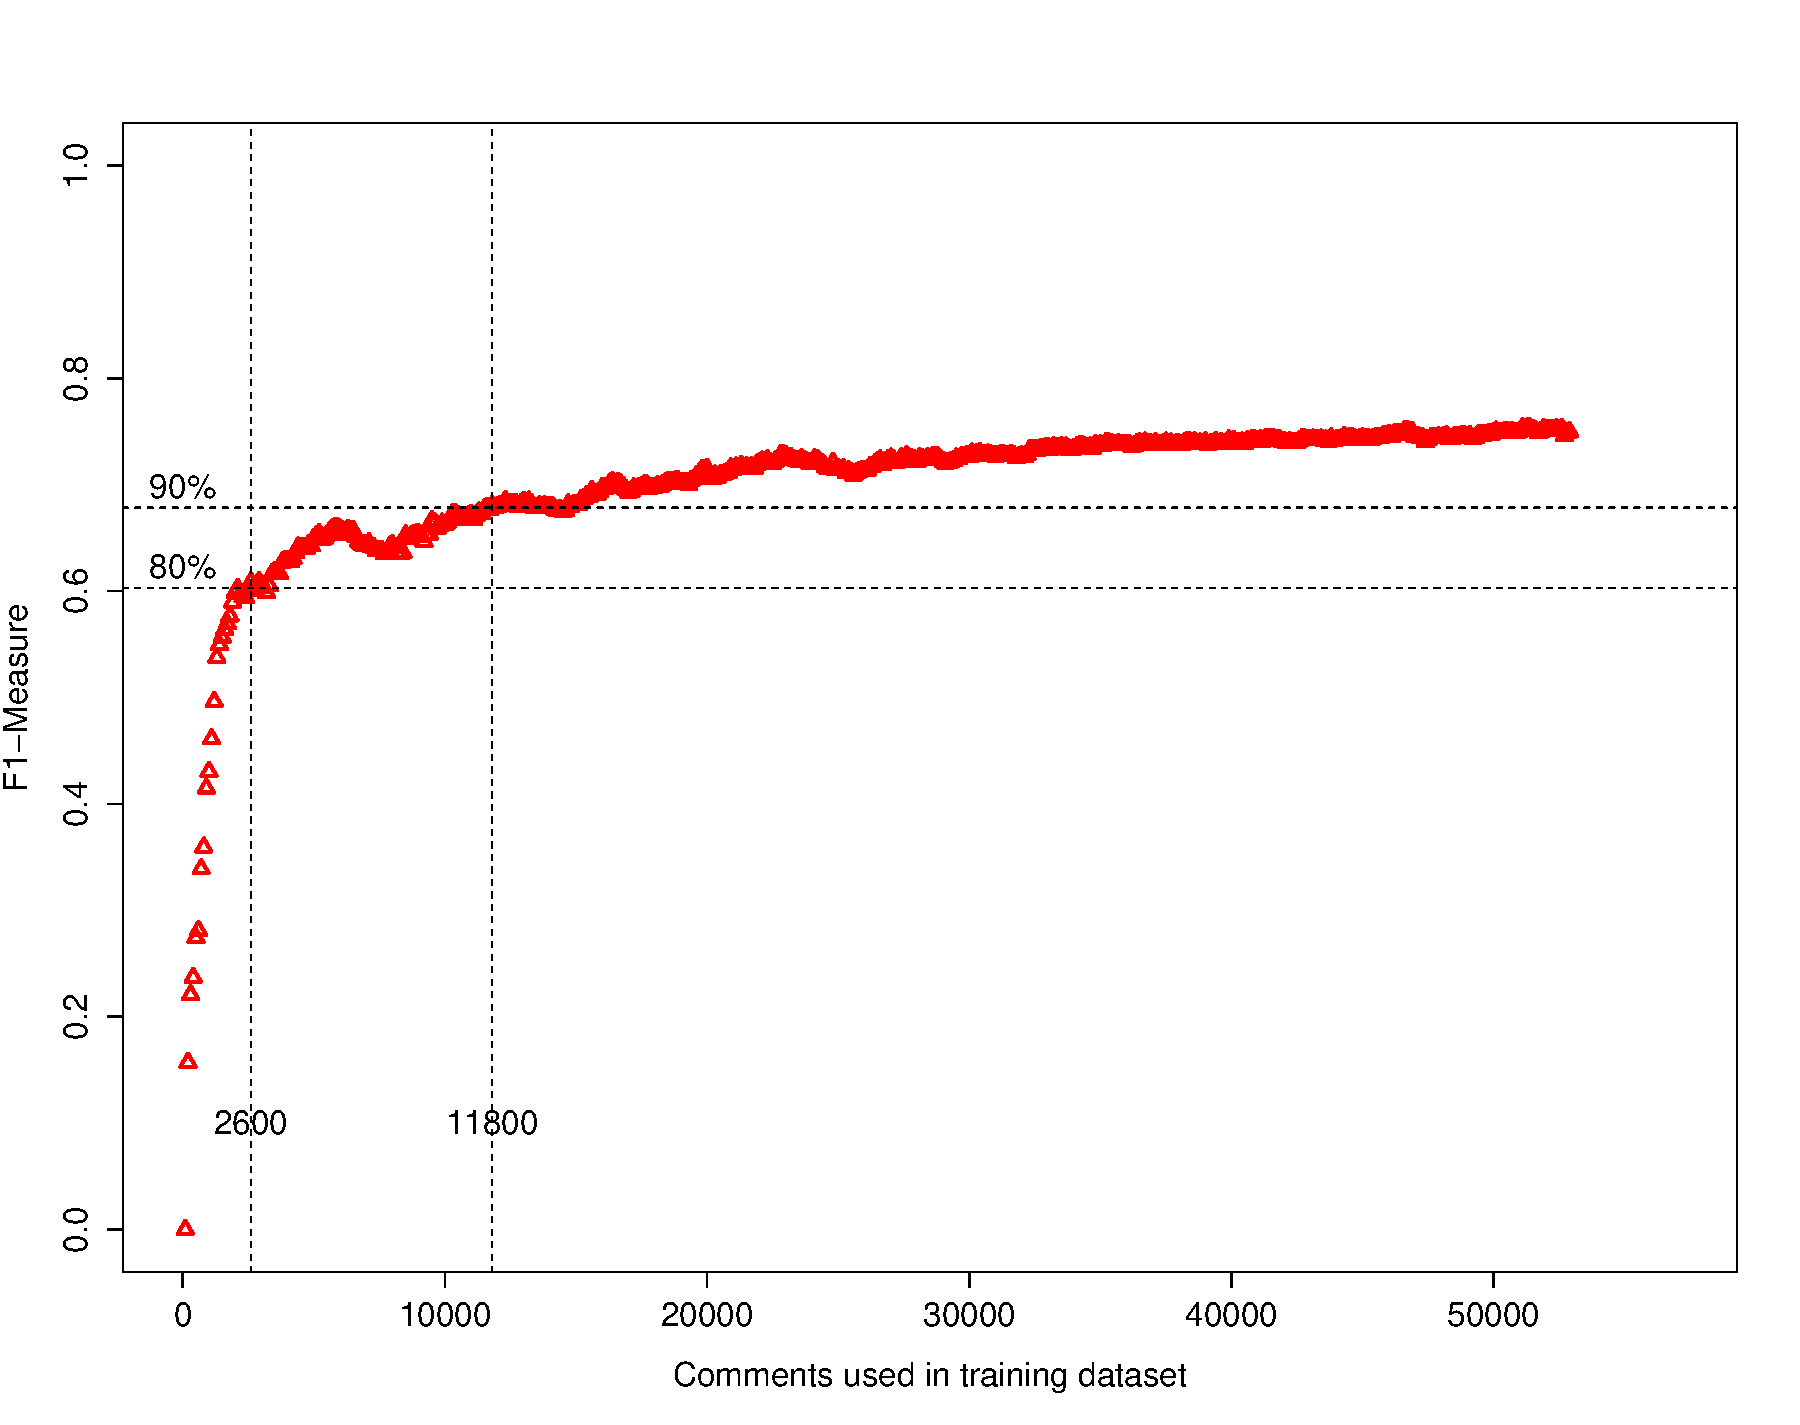
\includegraphics[width=0.48\textwidth]{figures/chapter4/ten_fold_validation_average_100_requirement.pdf}
    \label{chap4:fig:design_debt_per_comment_average}}
    \subfigure[Requirement Debt]{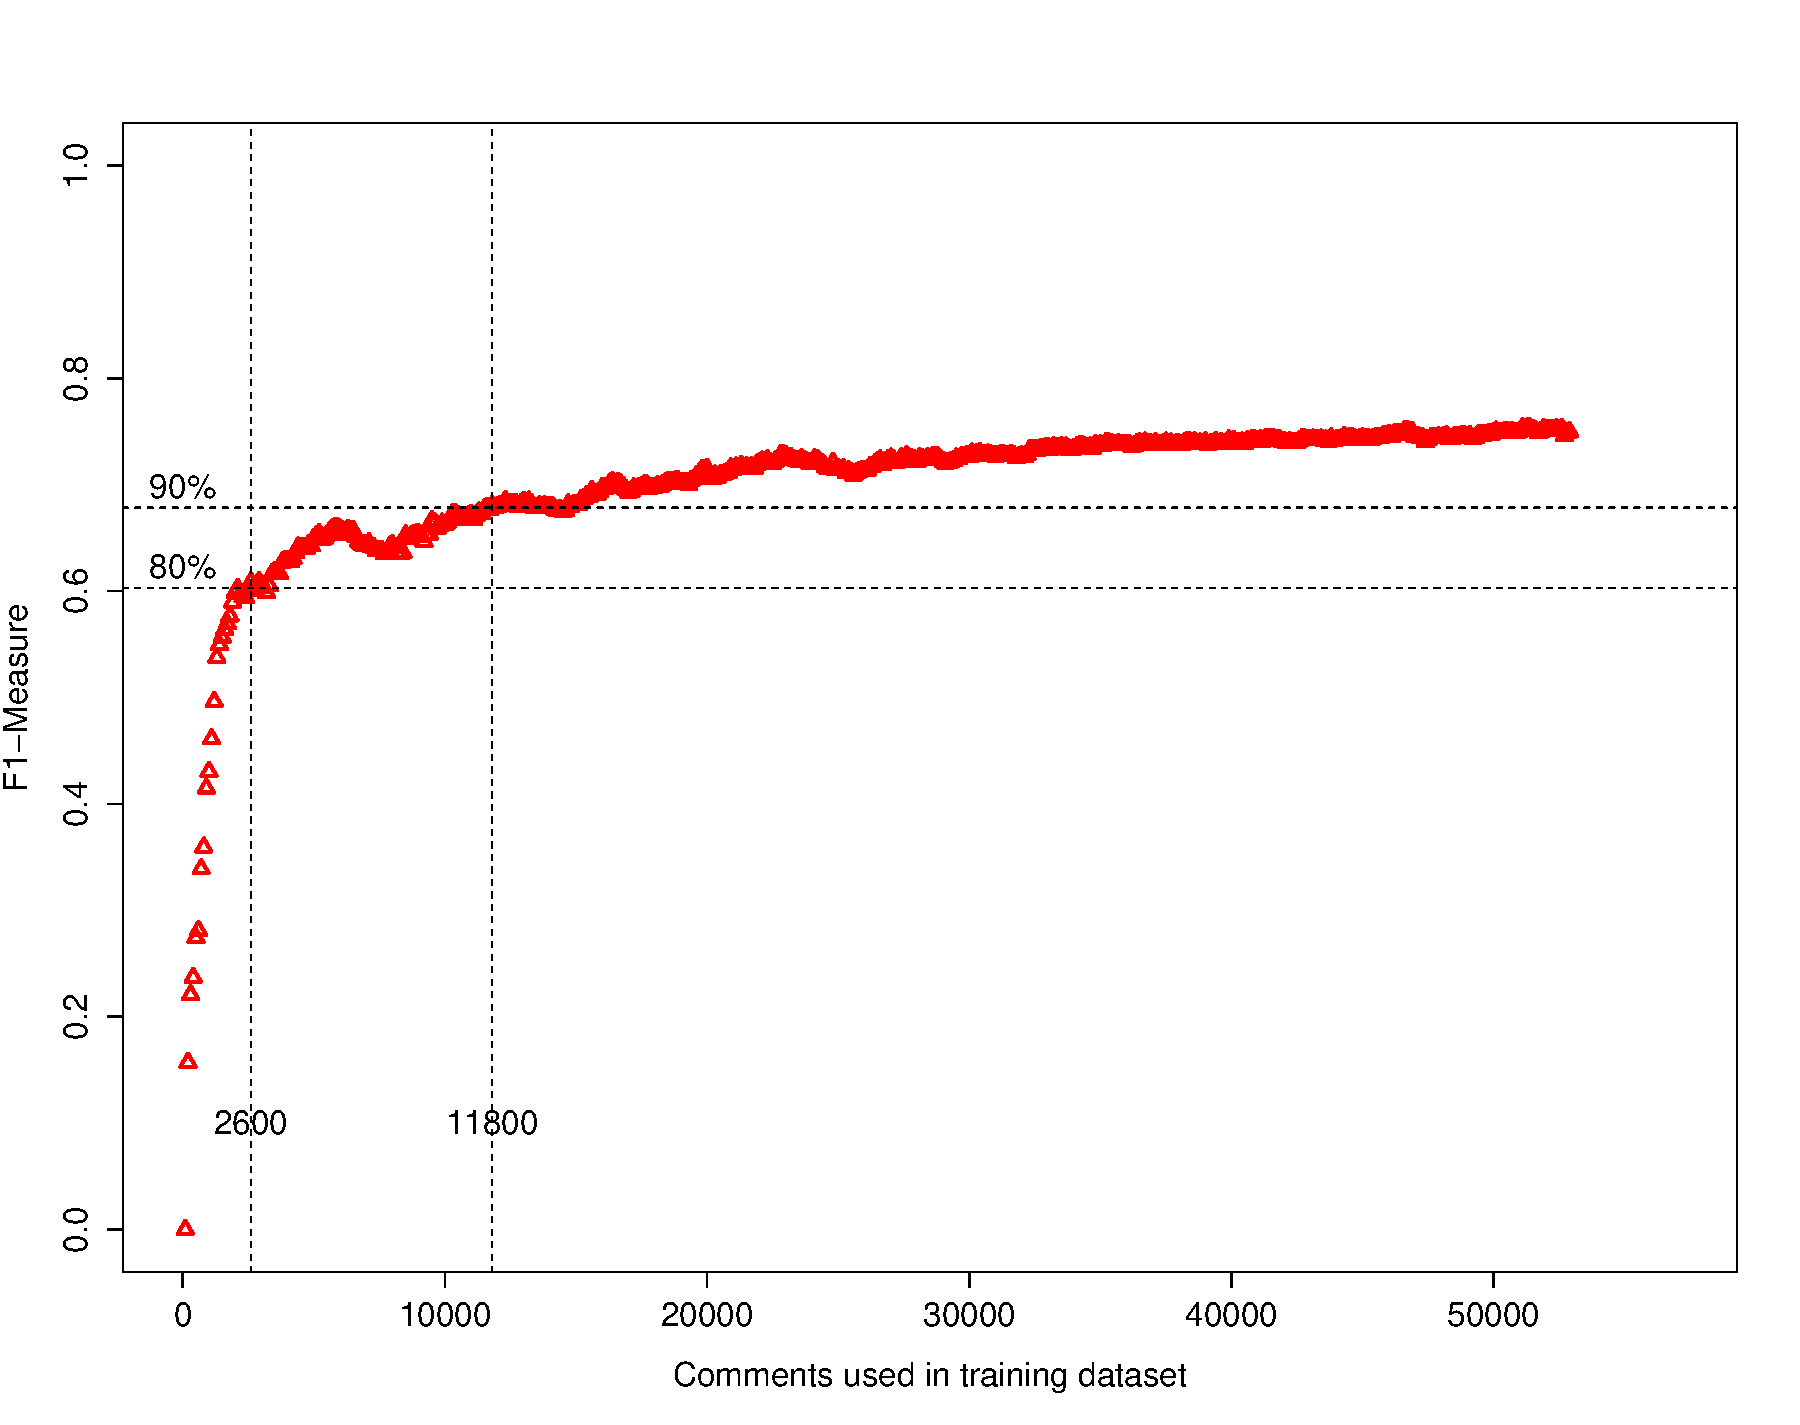
\includegraphics[width=0.48\textwidth]{figures/chapter4/ten_fold_validation_average_100_requirement.pdf}
    \label{chap4:fig:requirement_debt_per_comment_average}}
    \caption{F1-measure Achieved by Incrementally Adding Batches of 100 Comments in the Training Dataset.}
\end{figure}

\noindent \textbf{Results - design debt:} Figure~\ref{chap4:fig:design_debt_per_comment_average} shows the average F1-measure values obtained when detecting design \SATD, while adding batches of 100 comments. We find that the F1-measure score improves as we increase the number of comments in the training dataset, and the highest value (i.e., 0.824) is achieved with 42,700 comments. However, the steepest improvement in the F1-measure performance takes place within the first 2K-4K comments. Additionally, 80\% and 90\% of the maximum F1-measure value is achieved with 3,900 and 9,700 comments in the training dataset, respectively.
Since each batch of comments consists of approximately 5\% (i.e., $\frac{2,703}{58,122}$) comments with design \SATD, the iteration achieving 80\% of the maximum F1-measure value contains 195 comments with design \SATD,
while the iteration achieving 90\% of the maximum F1-measure value contains 485 such comments.
In conclusion, to achieve 80\% of the maximum F1-measure value, we need only 9.1\% (i.e., $\frac{3,900}{42,700}$) of the training data, while to achieve 90\% of the maximum F1-measure value, we need only 22.7\% (i.e., $\frac{9,700}{42,700}$) of the training data.

\noindent \textbf{Results - requirement debt:} Figure~\ref{chap4:fig:requirement_debt_per_comment_average} shows the average F1-measure values obtained when detecting requirement \SATD, while adding batches of 100 comments. As expected, the F1-measure increases as we add more comments into the training dataset, and again the steepest improvement takes place within the first 2-3K comments.

The highest F1-measure value (i.e., 0.753) is achieved using 51,300 comments of which 675 are requirement \SATD. Additionally, 80\% of the maximum F1-measure score is achieved with 2,600 comments, while 90\% of the maximum F1-measure score with 11,800 comments in the training dataset.

Each batch contains two comments with requirement \SATD, since the percentage of such comments is 1.3\% (i.e., $\frac{757}{58,122}$) in the entire dataset.As a result, the iteration achieving 80\% of the maximum F1-measure value contains 52 comments with requirement \SATD, while the iteration achieving 90\% of the maximum F1-measure value contains 236 such comments.

In conclusion, to achieve 80\% of the maximum F1-measure value, we need only 5\% (i.e., $\frac{2,600}{51,300}$) of the training data, while to achieve 90\% of the maximum F1-measure value, we need only 23\% (i.e., $\frac{11,800}{51,300}$) of the training data.

\conclusionbox{We find that to achieve a performance equivalent to 90\% of the maximum F1-measure score, only 23\% of the comments are required for both design and requirement \SATD. For a performance equivalent to 80\% of the maximum F1-measure score, only 9\% and 5\% of the comments are required for design and requirement \SATD, respectively.}

\section{Discussion}
\label{chap4:sec:discussion}

Thus far, we have seen that our NLP-based approach can perform well in classifying \SATD. However, there are some observations that warrant further investigation. For example, when it comes to the different types of \SATD, we find that requirement debt tends to require less training data, which is another interesting point that is worth further investigation (Section~\ref{chap4:sec:textual_similarity}). 

Moreover, we think that is also interesting to know the performance of our approach when trained to distinguish between \SATD and non-\SATD, i.e., without using fine-grained classes of debt, such as design and requirement debt (Section~\ref{chap4:sec:coarse-grained_classes}).

% Also, when performing our classification, there are several different classifiers that can be used in the Stanford Classifier toolkit, hence we investigate what is the impact of using different classifiers on the accuracy (Section~\ref{chap4:sec:underlying_classifier}).

Lastly, we analyze the overlap between the files that contain \SATD and the files that contain code smells. This is an interesting point of discussion to provide insights on how technical debt found in comments relates to code smells found by static analysis tools (Section~\ref{sec:overlap_with_static_analysis_tools}).

\subsection{Textual Similarity for Design and Requirement Debt}
\label{chap4:sec:textual_similarity}
For RQ3, we hypothesize that one of the reasons that the detection of requirement \SATD comments needs less training data is because such comments are more similar to each other compared to design \SATD comments. Therefore, we compare the intra-similarity of the requirement and design debt comments.

We start by calculating the term frequency-inverse document frequency (\textit{tf-idf}) weight of each design and requirement \SATD comment. Term frequency (\textit{tf}) is the simple count of occurrences that a term (i.e., word) has in a document (i.e., comment). Inverse document frequency (\textit{idf}) takes into account the number of documents that the term appears. However, as the name implies, the more one term is repeated across multiple documents the less relevant it is. Therefore, let \textit{N} be the total number of documents in a collection, the \textit{idf} of a term \textit{t} is defined as follows: \(idf_{t} = log\frac{N}{df_{t}}\). The total \textit{tf-idf} weight of a document is equal to the sum of each individual term \textit{tf-idf} weight in the document. Each document is represented by a \textit{document vector} in a \textit{vector space model}. 

Once we have the \textit{tf-idf} weights for the comments, we calculate the \textit{cosine similarity} between the comments. The Cosine similarity can be viewed as the \textit{dot product} of the normalized versions of two document vectors (i.e., two comments)~\cite{Manning2008book}. The value of the cosine distance ranges between 0 to 1, where 0 means that the comments are not similar at all and 1 means that the comments are identical.

For example, the requirement \SATD dataset contains 757 comments, for which we generate a 757$\times$757 matrix (since we compare each comment to all other comments).
Finally, we take the average cosine similarity for design and requirement debt comments, respectively, and plot their distributions.
Figure~\ref{fig:textual_similarity} shows that the median and the upper quartile for requirement \SATD comments are higher than the median and upper quartile for design \SATD.
The median for requirement debt comments is 0.018, whereas, the median for design debt comments is 0.011.
To ensure that the difference is statistically significant, we perform the Wilcoxon test to calculate the p-value. The calculated p-value is less than 2.2e-16 showing that the result is indeed statistically significant (i.e., p \textless 0.001). Considering our findings, our hypothesis is validated, showing that requirement \SATD comments are more similar to each other compared to design \SATD comments. This may help explain why requirement debt needs a smaller set of positive weight textual features to be detected.

\begin{figure}[!thb]
  \centering
  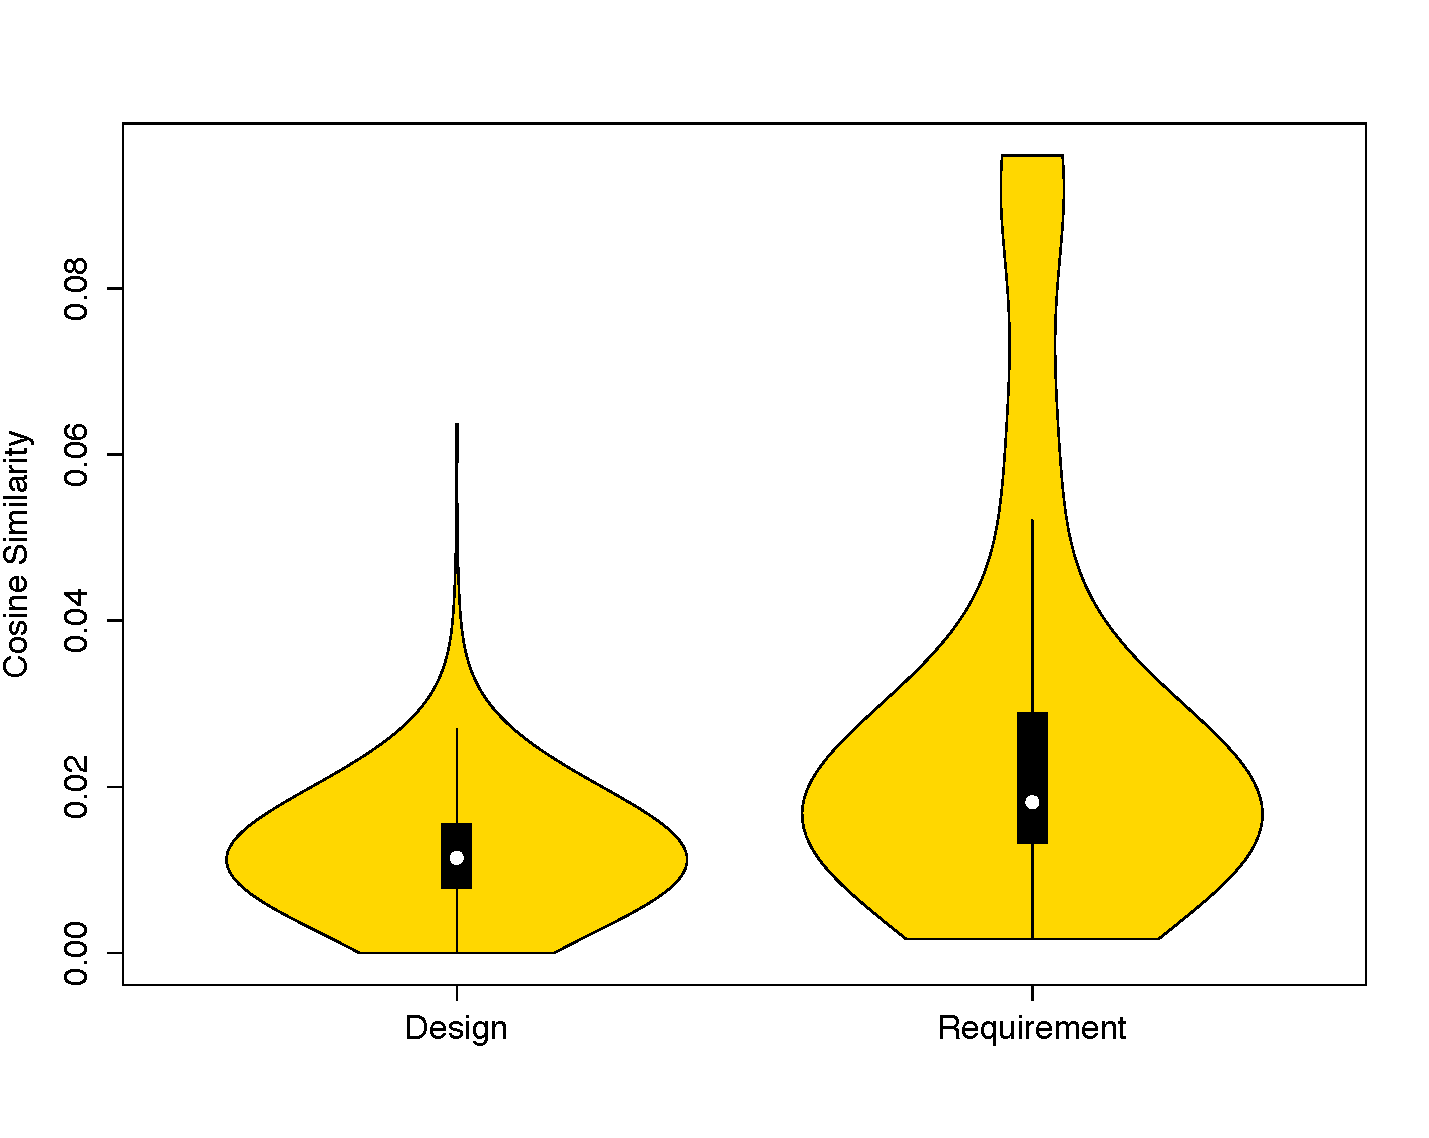
\includegraphics[width = 0.8\textwidth]{figures/chapter4/textual_similarity_removing_stop_words.pdf}
  \caption{Textual Similarity Between Design and Requirement Debt Comments}
  \label{fig:textual_similarity}
\end{figure}

\subsection{Distinguishing Self-Admitted Technical Debt from Non-Self-Admitted Technical Debt Comments}
\label{chap4:sec:coarse-grained_classes}

\begin{table}[!thb]
  \begin{center}
    \caption{F1-measure Performance Considering Different Types of Self-admitted Technical Debt}
    \label{chap4:tbl:nlpbased_performance_comparison}
    \begin{tabular}{l| c c c}
        \toprule
        \textbf{\thead{Project}} & \textbf{\thead{Design\\Debt}} & \textbf{\thead{Requirement\\Debt}} & \textbf{\thead{Technical\\Debt}} \\
        \midrule
        \textbf{Ant}           & 0.517 & 0.154 & 0.512 \\
        \textbf{ArgoUML}       & 0.814 & 0.595 & 0.819 \\
        \textbf{Columba}       & 0.601 & 0.804 & 0.750 \\
        \textbf{EMF}           & 0.470 & 0.381 & 0.462 \\
        \textbf{Hibernate}     & 0.744 & 0.476 & 0.763 \\
        \textbf{JEdit}         & 0.509 & 0.091 & 0.461 \\
        \textbf{JFreeChart}    & 0.492 & 0.321 & 0.513 \\
        \textbf{JMeter}        & 0.731 & 0.237 & 0.715 \\
        \textbf{JRuby}         & 0.783 & 0.435 & 0.773 \\
        \textbf{SQuirrel}      & 0.540 & 0.541 & 0.593 \\
        \midrule 
        \textbf{Average}       & 0.620 & 0.403 & 0.636 \\ 
        \bottomrule
    \end{tabular}
  \end{center}    
\end{table}

\begin{table}[!thb]
   \begin{center}
       \caption{Top-10 Textual Features Used to Identify Different Types of Self-Admitted Technical Debt}
       \label{chap4:tbl:top_ten_features_td_vs_non_td}
       \begin{tabular}{l| l l l }
       \toprule
       \textbf{\thead{Project}} & \textbf{\thead{Design\\debt}} & \textbf{\thead{Requirement\\debt}} & \textbf{\thead{Technical\\debt}} \\
       \midrule
        \textbf{1}  & hack       &   todo            & \textbf{hack}         \\
        \textbf{2}  & workaround &   needed          & \textbf{workaround}   \\
        \textbf{3}  & yuck!      &   implementation  & yuck!        \\
        \textbf{4}  & kludge     &   fixme           & kludge       \\
        \textbf{5}  & stupidity  &   xxx             & stupidity    \\
        \textbf{6}  & needed?    &   ends?           & needed?      \\
        \textbf{7}  & columns?   &   convention      & unused?      \\
        \textbf{8}  & unused?    &   configurable    & \textbf{fixme}        \\
        \textbf{9}  & wtf?       &   apparently      & \textbf{todo}         \\
        \textbf{10} & todo       &   fudging         & wtf?         \\
       \bottomrule
       \end{tabular}
   \end{center}    
\end{table}

So far, we analyzed the performance of our NLP-based approach to identify distinct types of \SATD (i.e., design and requirement debt). However, a simpler distinction between \SATD and non-debt comments can also be interesting in the case those fine-grained classes of debt are not considered necessary by a user of the proposed NLP-based detection approach. Another reason justifying such a coarse-grained distinction is that the cost of building a training dataset with fine-grained classes of debt is more expensive, mentally challenging, and subjective than building a training dataset with just two classes (i.e., comments with and without technical debt).

In order to compute the performance of our NLP-based approach using only two classes (i.e., comments with and without technical debt), we repeat RQ1 and RQ2 with modified training and test datasets.
First, we take all design and requirement \SATD comments and label them with a common class i.e., technical debt, and the remaining comments we kept them labeled as without technical debt.
Second, we run the maximum entropy classifier in the same leave-one-out cross-project validation fashion, using the comments of 9 projects to train the classifier and the comments from the remaining project to test the classifier. We repeat this process for each of the ten projects and compute the average F1-measure. Lastly, we analyze the textual features used to identify the self-admitted technical debt comments.

Table \ref{chap4:tbl:nlpbased_performance_comparison} compares the F1-measure achieved when detecting design debt, requirement debt, separately and when detecting both combined in a single class. As we can see, the performance when detecting technical debt is very similar with the performance of the classifier when detecting design debt. This is expected, as the majority of technical debt comments in the training dataset are labeled with the design debt class. Nevertheless, the performance achieved when detecting design debt was surpassed in the projects where the classifier performed well in detecting requirement debt, for example, in Columba (0.601 vs. 0.750) and SQuirrel SQL (0.540 vs. 0.593). 

We find that the average performance when detecting design and requirement \SATD combined is better (0.636) than the performance achieved when detecting them individually (0.620 and 0.403 for design and requirement debt, respectively).

Table \ref{chap4:tbl:top_ten_features_td_vs_non_td} shows a comparison of the top-10 textual features used to detect design and requirement debt comments separately, and those used to detect both types of debt combined in a single class.
When analyzing the top-10 textual features used to classify \SATD, we find once more, a strong overlap with the top-10 textual features used to classify design debt. The weight of the features is attributed in accordance to the frequency that each word is found in the training dataset, and therefore, the top-10 features tend to be similar with the top-10 design debt features, since design debt comments represent the majority of \SATD comments in the dataset. 

\subsection{Investigating the Overlap Between Technical Debt Found in Comments and Technical Debt Found by Static Analysis Tools}
\label{sec:overlap_with_static_analysis_tools}
Thus far, we analyzed technical debt that was expressed by developers through source code comments. However, there are other ways to identify technical debt, such as architectural reviews, documentation analysis, and static analysis tools. To date, using static analysis tools is one of the most popular approaches to identify technical debt in the source code~\cite{Fontana2012MTD}. In general, static analysis tools parse the source code of a project to calculate metrics and identify possible object oriented design violations, also known as code smells, anti-patterns, or design technical debt, based on some fixed metric threshold values. 

We analyze the overlap between what our NLP-based approach identifies as technical debt and what a static analysis tool identifies as technical debt. We selected JDeodorant as the static analysis tool, since it supports the detection of three popular code smells, namely Long Method, God Class, and Feature Envy. We avoided the use of metric-based code smell detection tools, because they tend to have high false positive rates and flag a large portion of the code base as problematic~\cite{Fontana2016SANER}. On the other hand, JDeodorant detects only actionable code smells (i.e., code smells for which a behavior-preserving refactoring can be applied to resolve them), and does not rely on any metric thresholds, but rather applies static source code analysis to detect structural anomalies and suggest refactoring opportunities to eliminate them~\cite{Tsantalis2008CSMR}.

First, we analyzed our 10 open source projects using JDeodorant. The result of this analysis is a list of Java files that were identified having at least one instance of
the Long Method, God Class, and Feature Envy code smells. These code smells have been extensively investigated in the literature, and are considered to occur frequently~\cite{Olbrich2010ICSM,Sjoberg2013TSE}. Second, we created a similar list containing the files that were identified with \SATD comments. Finally, we examined the overlap of the two lists of files. It should be emphasized that we did not examine if the \SATD comments actually discuss the detected code smells, but only if there is a co-occurrence at file-level.

Table \ref{tbl:static_analysis_tool_and_self_admitted_technical_debt_overlap_using_jdeodorant} provides details about each one of the projects used in our study. The columns of Table \ref{tbl:static_analysis_tool_and_self_admitted_technical_debt_overlap_using_jdeodorant} present the total number of files with \SATD, followed by the number of files containing \SATD comments and at least one code smell instance,
along with the percentage over the total number of files with \SATD, for Long Method, Feature Envy, God Class, and all code smells combined, respectively. 

JMeter, for example, has 200 files that contain \SATD comments, and 143 of these files also contain at least one Long Method code smell (i.e., 71.5\%). In addition, we can see that 20.5\% of the files that have \SATD are involved in Feature Envy code smells, and 48.5\% of them are involved in God Class code smells. In summary, we see that 80.5\% of the files that contain \SATD comments are also involved in at least one of the three examined code smells.     

We find that the code smell that overlaps the most with \SATD is Long Method. Intuitively, this is expected, since Long Method is a common code smell and may have multiple instances per file, because it is computed at the method level. The overlap between files with \SATD and Long Method ranged from 43.6\% to 82\% of all the files containing \SATD comments, and considering all projects, the average overlap is 65\%. In addition, 44.2\% of the files with \SATD comments are also involved in God Class code smells, and 20.7\% in Feature Envy code smells. Taking all examined code smells in consideration we find that, on average, 69.7\% of files containing \SATD are also involved in at least one of the three examined code smells. 

Our findings here shows that using code comments to identify technical debt is a complementary approach to using code smells to detect technical debt. Clearly, there is overlap, however, each approach also identifies unique instances of technical debt.

\begin{landscape}
\begin{table*}[!thb]
    \centering
        \caption{Overlap Between the Files Containing \SATD and the Files Containing Code Smells as Detected by JDeodorant}
        \label{tbl:static_analysis_tool_and_self_admitted_technical_debt_overlap_using_jdeodorant}
        \resizebox{\columnwidth}{!}{%
        \begin{tabular}{l| c c c c c c c c c}
        \toprule
        \textbf{\thead{Project}} & \textbf{\thead{\# of \\Files with\\ SATD }} & \textbf{\thead{\# of SATD \\Files with \\ Long \\Method }} & \textbf{\thead{\%  of SATD \\Files with \\ Long \\Method}} & \textbf{\thead{\# of SATD \\Files with \\ Feature \\Envy}} & \textbf{\thead{\% of SATD \\fFles with \\ Feature \\Envy}} & \textbf{\thead{\# of SATD\\ Files with \\ God \\Class}} & \textbf{\thead{\% of SATD\\ Files with \\ God \\Class}} & \textbf{\thead{\# of SATD\\ Files with\\ Any Code \\Smell }} & \textbf{\thead{\% of SATD\\ Files with\\ Any Code \\Smell}}\\
        \midrule
        
        \textbf{Ant}            & 73  & 57   & 78.0  & 19 & 26.0  & 42  & 57.5 & 63  & 86.3   \\
        \textbf{ArgoUML}        & 419 & 255  & 60.8  & 43 & 10.2  & 128 & 30.5 & 283 & 67.5   \\
        \textbf{Columba}        & 117 & 76   & 64.9  & 18 & 15.3  & 47  & 40.1 & 89  & 76.0   \\
        \textbf{EMF}            & 53  & 33   & 62.2  & 14 & 26.4  & 28  & 52.8 & 28  & 52.8   \\
        \textbf{Hibernate}      & 206 & 90   & 43.6  & 44 & 21.3  & 72  & 34.9 & 116 & 56.3   \\
        \textbf{JEdit}          & 108 & 74   & 68.5  & 23 & 21.2  & 47  & 43.5 & 82  & 75.9   \\
        \textbf{JFreeChart}     & 106 & 87   & 82.0  & 20 & 18.8  & 52  & 49.0 & 92  & 86.7   \\
        \textbf{JMeter}         & 200 & 143  & 71.5  & 41 & 20.5  & 97  & 48.5 & 161 & 80.5   \\
        \textbf{JRuby}          & 163 & 107  & 65.5  & 43 & 26.3  & 79  & 48.4 & 85  & 52.1   \\
        \textbf{SQuirrel}       & 156 & 82   & 52.5  & 32 & 20.5  & 58  & 37.1 & 99  & 63.4   \\
        \midrule
        \textbf{Average}        &     &      & 65.0  &    & 20.7  &     & 44.2 &     & 69.7  \\

        \bottomrule
        \end{tabular}}
\end{table*} 
\end{landscape}

\section{Related Work}
\label{chap4:sec:related_work}

Our work uses code comments to detect \SATD using a Natural Language Processing (NLP) technique. Therefore, we divide the related work into three subsections, namely source code comments, technical debt, and NLP in software engineering.

\subsection{Source Code Comments}

A number of studies examined the co-evolution of source code comments and the rationale for changing code comments. For example, Fluri \textit{et al.}~\cite{Fluri2007WCRE} analyzed the co-evolution of source code and code comments, and found that 97\% of the comment changes are consistent. Tan \textit{et al.}~\cite{Tan2012ICST} proposed a novel approach to identify inconsistencies between Javadoc comments and method signatures. Malik \textit{et al.} \cite{Malik2008ICSM} studied the likelihood of a comment to be updated and found that call dependencies, control statements, the age of the function containing the comment, and the number of co-changed dependent functions are the most important factors to predict comment updates.

Other works used code comments to understand developer tasks. For example. Storey \textit{et al.}~\cite{Storey2008ICSE} analyzed how task annotations (e.g., TODO, FIXME) play a role in improving team articulation and communication. The work closest to ours is the work by Potdar and Shihab~\cite{Potdar2014ICSME}, where code comments were used to identify technical debt, called \SATD. 

Similar to some of the prior work, we also use source code comments to identify technical debt. However, our main focus is on the detection of different \emph{types} of \SATD. As we have shown, our approach yields different and better results in the detection of \SATD.
%Furthermore, we propose an approach to identify \SATD, that is derived from source code comments and natural language processing techniques, to detect \SATD.

\subsection{Technical Debt}

A number of studies has focused on the detection and management of technical debt. For example, Seaman \textit{et al.}~\cite{Seaman2011}, Kruchten \textit{et al.}~\cite{Kruchten2013IWMTD} and Brown \textit{et al.}~\cite{Brown2010MTD} make several reflections about the term technical debt and how it has been used to communicate the issues that developers find in the code in a way that managers can understand. 

Other work focused on the detection of technical debt. Zazworka \textit{et al.} \cite{Zazworka2013CSE} conducted an experiment to compare the efficiency of automated tools in comparison with human elicitation regarding the detection of technical debt. They found that there is a small overlap between the two approaches, and thus it is better to combine them than replace one with the other. In addition, they concluded that automated tools are more efficient in finding defect debt, whereas developers can realize more abstract categories of technical debt.

In a follow up work, Zazworka \textit{et al.}~\cite{Zazworka2011MTD} conducted a study to measure the impact of technical debt on software quality. They focused on a particular kind of design debt, namely, God Classes. They found that God Classes are more likely to change, and therefore, have a higher impact on software quality. Fontana \textit{et al.}~\cite{Fontana2012MTD} investigated design technical debt appearing in the form of code smells. They used metrics to find three different code smells, namely God Classes, Data Classes and Duplicated Code. They proposed an approach to classify which one of the different code smells should be addressed first, based on its risk. Ernst \textit{et al.} ~\cite{Ernst2015FSE} conducted a survey with 1,831 participants and found that architectural decisions are the most important source of technical debt.

Our work is different from the work that uses code smells to detect design technical debt, since we use code comments to detect technical debt. Moreover, our approach does not rely on code metrics and thresholds to identify technical debt and can be used to identify bad quality code symptoms other than bad smells.

More recently, Potdar and Shihab~\cite{Potdar2014ICSME} extracted the comments of four projects and analyzed 101,762 comments to come up with 62  patterns that indicate self-admitted technical debt. Their findings show that 2.4\% - 31\% of the files in a project contain self-admitted technical debt. Bavota and Russo~\cite{bavota2016MSR} replicated the study of \SATD on a large set of Apache projects and confirmed the findings observed by Potdar and Shihab in their earlier work. Wehaibi \textit{et al.}~\cite{wehaibi2016SANER} examined the impact of \SATD and found that \SATD leads to more complex changes in the future. All three of the aforementioned studies used the comment patterns approach to detect \SATD. Our earlier work~\cite{Maldonado2015MTD} examined more than ~33 thousands comments to classify the different types of \SATD found in source code comments. Farias \textit{et al.}~\cite{Farias2015MTD} proposed a contextualized vocabulary model for identifying technical debt in comments using word classes and code tags in the process. 

Our work also uses code comments to detect design technical debt. However, we use these code comments to train a maximum entropy classifier to automatically identify technical debt. Also, our focus is on \emph{self-admitted} design and requirement technical debt.

\subsection{NLP in Software Engineering}

A number of studies leveraged NLP in software engineering, mainly for the traceability of requirements, program comprehension and software maintenance. For example, Lormans and van Deursen~\cite{Lormans2006CSRM} used latent semantic indexing (LSI) to create traceable links between requirements and test cases and requirements to design implementations. Hayes \textit{et al.}~\cite{Hayes2005, Hayes2006TSE} created a tool called RETRO that applies information retrieval techniques to trace and map requirements to designs. Yadla \textit{et al.}~\cite{yadla2005tracing} further enhanced the RETRO tool and linked requirements to issue reports. On the other hand, Runeson \textit{et al.}~\cite{Runeson2007ICSE} implemented a NLP-based tool to automatically identify duplicated issue reports, they found that 2/3 of the possible duplicates examined in their study can be found with their tool. Canfora and Cerulo \cite{Canfora2005ISSM} linked a change request with the corresponding set of source files using NLP techniques, and then, they evaluated the performance of the approach on four open source projects.  

The prior work motivated us to use NLP techniques. However, our work is different from the aforementioned ones, since we apply NLP techniques on code comments to identify \SATD, rather than use it for traceability and linking between different software artifacts.

\section{Threats to Validity}
\label{chap4:sec:threats_to_validity}

\noindent\textbf{Construct validity and reliability} considers the relationship between theory and observation, in case the measured variables do not measure the actual factors. The training dataset used by us heavily relied on a manual analysis and classification of the code comments from the studied projects. Like any human activity, our manual classification is subject to personal bias. To reduce this bias, we took a sample of our classified comments and asked a Phd's candidate, who is not an author of the paper, to manually classify them. Then, we calculate the Kappa's level of agreement between the two classifications. The level of agreement obtained was +0.84, which according to Fleiss~\cite{Fleiss1981measurement} is characterized as an excellent inter-rater agreement (values larger than +0.75 are considered excellent). Nevertheless, we also measured Kappa's level of agreement for design and requirement \SATD separately. The level of agreement obtained for design and requirement \SATD was +0.89 and +0.83, respectively.

When performing our study, we used well-commented Java projects. Since our approach heavily depends on code comments, our results and performance measures may be impacted by the quantity and quality of comments in a software project. 

Considering the intentional misrepresentation of measures, it is possible that even a well commented project does not contain self-admitted technical debt. Given the fact that the developers may opt to not express themselves in source code comments. In our study, we made sure that we choose case studies that are appropriately commented for our analysis.

On the same point, using comments to determine some self-admitted technical debt may not be fully representative, since comments or code may not be updated consistently. However, previous work shows that changes in the source code are consistent to changes in comments~\cite{Fluri2007WCRE,Potdar2014ICSME}. In addition, it is possible that a variety of technical debt that is not self-admitted is present in the analyzed projects. However, since the focus of this paper is to improve the detection of the most common types of \SATD, considering all technical debt is out of the scope of this paper.

Lastly, our approach depends on the correctness of the underlying tools we use. To mitigate this risk, we used tools that are commonly used by practitioners and by the research community, such as JDeodorant for the extraction of source code comments and for investigating the overlap with code smells (Section~\ref{sec:overlap_with_static_analysis_tools}) and the Stanford Classifier for training and testing the max entropy classifier used in our approach.

\noindent \textbf{External validity} considers the generalization of our findings. All of our findings were derived from comments in open source projects. To minimize the threat to external validity, we chose open source projects from different domains. That said, our results may not generalize to other open source or commercial projects, projects written in different languages, projects from different domains and/or technology stacks. In particular, our results may not generalize to projects that have a low number or no comments or comments that are written in a language other than English.

\section{Conclusion and Future Work}
\label{chap4:sec:conclusion}

Technical debt is a term being used to express non-optimal solutions, such as hacks and workarounds, that are applied during the software development process. Although these non-optimal solutions can help achieve immediate pressing goals, most often they will have a negative impact on the project maintainability~\cite{Zazworka2011MTD}. 

Our work focuses on the identification of \SATD through the use of Natural Language Processing. We analyzed the comments of 10 open source projects namely Ant, ArgoUML, Columba, EMF, Hibernate, JEdit, JFreeChart, JMeter, JRuby and SQuirrel SQL. These projects are considered well commented and they belong to different application domains. The comments of these projects were manually classified into specific types of technical debt such as design, requirement, defect, documentation and test debt. Next, we selected 61,664 comments from this dataset (i.e., those classified as design \SATD, requirement \SATD and without technical debt) to train the maximum entropy classifier, and then this classifier was used to identify  design and requirement \SATD automatically.

We first evaluated the performance of our approach by comparing the F1-measure of our approach with the F1-measure of two other baselines, i.e., the comment patterns baseline and the simple (random) baseline. We have shown that our approach outperforms the comment patterns baseline on average 2.3 and 6 times in the identification of design and requirement \SATD, respectively. Moreover, our approach can identify requirement \SATD, while the comment patterns baseline fails to detect this kind of debt in most of the examined projects. Furthermore, the performance of our approach surpasses the simple (random) baseline on average 7.6 and 19.1 times for design and requirement \SATD, respectively. 

Then, we explored the characteristics of the features (i.e., words) used to classify \SATD. We find that the words used to express design and requirement \SATD are different from each other. The three strongest indicators of design \SATD are `hack', `workaround' and `yuck!', whereas, `todo', `needed' and `implementation' are the strongest indicators of requirement debt. In addition, we find that using only 5\% and 23\% of the comments in the training dataset still leads to an accuracy that is equivalent to 80\% and 90\% of the best performance, respectively. In fact, our results show that developers use a richer vocabulary to express design \SATD and a training dataset of at least 3,900 comments (of which 195 comments are design \SATD) is necessary to obtain a satisfactory classification. On the other hand, requirement \SATD is expressed in a more uniform way, and with a training dataset of 2,600 comments (of which 52 are \SATD) it is possible to classify with relatively high accuracy requirement \SATD.

In the future, we believe that more analysis is needed to fine tune the use of the current training dataset in order to achieve maximum efficiency in the detection of \SATD comments. For example, using subsets of our training dataset can be more suitable for some applications than using the whole dataset due to domain particularities. However, the results thus far are not to be neglected as our approach has the best F1-measure performance on every analyzed project. In addition, we plan to examine the applicability of our approach to more domains (than those we study in this paper) and software projects developed in different programming languages.

Another interesting research direction that we plan to investigate in the future is the use of other machine learning techniques, such as active learning to reduce the number of labeled data necessary to train the classifier. This technique, if proved successful, can further expand the horizon of projects that our approach can be applied to.

Moreover, to enable future research, we make the dataset created in this study publicly available\footnote{\url{https://github.com/maldonado/tse_satd_data}}. We believe that it will be a good starting point for researchers interested in identifying technical debt through comments and even experimenting with different Natural Language Processing techniques. Lastly, we plan to use the findings of this study to build a tool that will support software engineers in the task of identifying and managing \SATD. 


\chapter{Conclusions}
\label{conclusion}
% -*- root: cuthesis_masters.tex -*-

\section{Summary of Addressed Topics}

The main focus of our thesis is to tackle the challenges of \SATD identification. First, we conducted a survey of the state-of-the-art in the identification of technical debt research in order to understand the main challenges. Then, we manually analyzed a number of comments from different projects belonging to different application domains. Next, we propose an approach based on NLP techniques that outperforms the current state of the art in the identification of \SATD. The remainder of this chapter details the major topics covered in this thesis.

Chapter 2 surveys the state-of-art in technical debt. We believe that such a review is necessary at this time, since a lot of research is aiming to better understand technical debt. Therefore, it is an ideal time to reflect on the definitions and applications of the metaphor as well to evaluate the current challenges in the field.

Chapter 3 presents the result of the quantification of the different types of \SATD. In this chapter we analyzed the comments of 5 open source projects. These projects are considered well commented and they belong to different application domains. We used them to understand the characteristics of self-admitted technical debt types creating a rich dataset with more than 33,093 classified comments. We find that self-admitted technical debt can be classified into five types: design debt, defect debt, documentation debt, requirement debt and test debt. However, the two most prevalent types of \SATD are design and requirement \SATD. Design debt ranged from 42\% to 84\% across the projects, whereas, requirement debt ranged from 5\% to 45\%. 

Chapter 4 presents an approach that uses classified design and requirement \SATD comments to train a maximum entropy classifier to automatically identify \SATD. We evaluated the performance of our approach against two other baselines, i.e., the comment patterns baseline and the simple (random) baseline. We show that our approach performance surpassed the comment patterns baseline on average 2.3 and 6 times in the identification of design and requirement \SATD, respectively. Analyzing the features to identify \SATD we find that the words used to express design and requirement \SATD are different from each other. In addition, we find that using only 5\% and 23\% of the comments in the training dataset still leads to an accuracy that is equivalent to 80\% and 90\% of the best performance, respectively.

\section{Contributions}

The goal of this thesis is to propose an approach that can effectively identify \SATD comments. We make several contributions towards this goal. These contributions were motivated by previous research and our industrial experience. We summarize the main contributions of the thesis in more detail.

The major contributions of this thesis are as follows:
\begin{itemize}

\item \textbf{A concise review of the state of the art in technical debt:} We provide the readers a concise background evaluation from the the creation of the metaphor until present date. We choose the most relevant sources that define how the technical debt is being used and also the challenges involving the identification of technical debt.

\item \textbf{A rich dataset of manually labeled technical debt:} To create such dataset we read and analyzed the source code comments of 10 open source projects considered well commented and from different application domains. The comments of these projects were manually classified into specific types of technical debt such as design, requirement, defect, documentation and test debt. In total, our dataset contain 62,566 labeled comments and we made it publicly available to enable future research on the field. 

In addition, to mitigate the risk of creating a biased dataset, we also asked a student that was not involved with our work to classify a stratified sample. Then, we calculate the Kappa's level of agreement between the two classifications. The level of agreement obtained was +0.81, which according to Fleiss~\cite{Fleiss1981measurement} is characterized as an excellent inter-rater agreement.

\item \textbf{An automatic, NLP-based, approach to identify design and requirement \SATD:} We have shown that our approach outperforms the current state-of-the-art on average 2.3 and 6 times in the identification of design and requirement \SATD, respectively. Moreover, our approach can identify requirement \SATD, while the comment patterns baseline fails to detect this kind of debt in the majority of the examined projects. Furthermore, the performance of our approach outperforms the simple (random) baseline on average 7.6 and 19.1 times for design and requirement \SATD, respectively. 

\item \textbf{An empirical study to investigate the amount of training data necessary to effectively identify technical debt:} We discuss the implications of the amount training data that is necessary to apply our approach. For example, if we need a very large number of comments to create our training dataset, our approach will be more difficult to extend and apply for other projects. On the other hand, if a small dataset can be used to reliably identify comments with \SATD, then this approach can be applied with minimal effort, i.e., less training data. However, we find that using only 5\% and 23\% of the comments in the training dataset leads to an accuracy that is equivalent to 80\% and 90\% of the best performance, respectively. Our results also show that developers use a richer vocabulary to express design \SATD and a training dataset of at least 3,900 comments (of which 195 comments are design \SATD) is necessary to obtain a satisfactory classification. On the other hand, requirement \SATD is expressed in a more uniform way, and with a training dataset of 2,600 comments (of which 52 are \SATD) it is possible to classify with relatively high accuracy requirement \SATD.

\end{itemize}

\section{Future Work}

We believe that our thesis makes a positive contribution towards the goal of effectively identifying technical debt. However, there are still many open challenges that need to be tackled in order to improve the identification of technical debt. We now highlight some avenues for future work.

\subsection{Fine tunning the approach to obtain optimal results}

Although we conducted a number of diverse experiments with the NLP classifier, we believe that is still a lot of opportunities to be explored that may improve even further our approach. For example, we noticed that using subsets of our training dataset can be more suitable for some applications than using the whole dataset due to domain particularities. 

\subsection{Expanding the scope of our approach}

We plan to examine the applicability of our approach to more domains than those we study in this paper and software projects developed in different programming languages. Also, would be interesting to analyze projects that uses comments in different idioms than English. As we showed, we provide filtering heuristics that could be easily adapted to remove irrelevant comments from software projects and that we need a reduced amount of comments to obtain satisfactory results concerning the identification of technical debt. We believe that these factors will help future work to expand considerably. 

\subsection{Tool support for software developers}

Lastly, we plan to use the findings of this study to build a tool that will support software engineers in the task of identifying and managing \SATD. We envision that such tool would be useful to monitor debt and focus resources during the development of the software project, moreover, when properly managed software developers could take advantage of incurring debt when necessary, without losing track of the overall quality of the system.



\addcontentsline{toc}{chapter}{Bibliography}
\bibliography{bibliography.bib}  
\bibliographystyle{alpha}
\end{document}
